\documentclass{llncs}

\usepackage[T1]{fontenc}
\usepackage[utf8x]{inputenc}
\usepackage[english]{babel}
\usepackage{lmodern}
\usepackage{mathtools}
%\usepackage{fullpage}
\usepackage{graphicx}
\usepackage{xspace}
\usepackage{tabularx}
\usepackage[lf]{ebgaramond}
\usepackage{biolinum}
\usepackage[cmintegrals,cmbraces]{newtxmath}
\usepackage{ebgaramond-maths}
\usepackage{multicol}
\usepackage{sectsty}
\usepackage[noend]{algpseudocode}
\usepackage{algorithm}
\usepackage{algorithmicx}
\usepackage[bottom]{footmisc}
\usepackage{caption}
%\captionsetup{font=small}
\captionsetup{labelfont={sf,bf}}
\usepackage{ragged2e}
\usepackage{xcolor}

% llncs removes generation of PDF bookmarks, we must add them back
\usepackage{etoolbox}
\makeatletter
\let\llncs@addcontentsline\addcontentsline
\patchcmd{\maketitle}{\addcontentsline}{\llncs@addcontentsline}{}{}
\patchcmd{\maketitle}{\addcontentsline}{\llncs@addcontentsline}{}{}
\patchcmd{\maketitle}{\addcontentsline}{\llncs@addcontentsline}{}{}
\setcounter{tocdepth}{3}
\makeatother
\PassOptionsToPackage{hyphens}{url}
\usepackage[pdftex,bookmarks=true]{hyperref}
\hypersetup{
    bookmarksopen=true,
    bookmarksopenlevel=3,
    bookmarksnumbered=true,
    hidelinks,
    colorlinks,
    linkcolor={red!50!black},
    citecolor={green!50!black},
    urlcolor={blue!80!black}
}
%\hypersetup{hidelinks}

\makeatletter
  % Recover some math symbols that were masked by eb-garamond, but do not
  % have replacement definitions.
  \DeclareSymbolFont{ntxletters}{OML}{ntxmi}{m}{it}
  \SetSymbolFont{ntxletters}{bold}{OML}{ntxmi}{b}{it}
  \re@DeclareMathSymbol{\leftharpoonup}{\mathrel}{ntxletters}{"28}
  \re@DeclareMathSymbol{\leftharpoondown}{\mathrel}{ntxletters}{"29}
  \re@DeclareMathSymbol{\rightharpoonup}{\mathrel}{ntxletters}{"2A}
  \re@DeclareMathSymbol{\rightharpoondown}{\mathrel}{ntxletters}{"2B}
  \re@DeclareMathSymbol{\triangleleft}{\mathbin}{ntxletters}{"2F}
  \re@DeclareMathSymbol{\triangleright}{\mathbin}{ntxletters}{"2E}
  \re@DeclareMathSymbol{\partial}{\mathord}{ntxletters}{"40}
  \re@DeclareMathSymbol{\flat}{\mathord}{ntxletters}{"5B}
  \re@DeclareMathSymbol{\natural}{\mathord}{ntxletters}{"5C}
  \re@DeclareMathSymbol{\star}{\mathbin}{ntxletters}{"3F}
  \re@DeclareMathSymbol{\smile}{\mathrel}{ntxletters}{"5E}
  \re@DeclareMathSymbol{\frown}{\mathrel}{ntxletters}{"5F}
  \re@DeclareMathSymbol{\sharp}{\mathord}{ntxletters}{"5D}
  \re@DeclareMathAccent{\vec}{\mathord}{ntxletters}{"7E}

  % Change font for algorithm label.
  \renewcommand\ALG@name{\sffamily\bfseries Algorithm}
\makeatother

% Use the sans-serif fonts (for which bold is properly defined) for
% section headings. Also ensure that subsubsections get a number and
% that the number is displayed (to distinguish them from paragraphs).
\allsectionsfont{\sffamily}
\setcounter{secnumdepth}{3}
\pagestyle{plain}

\makeatletter
\renewenvironment{abstract}{%
      \list{}{\advance\topsep by0.35cm\relax\small
      \leftmargin=1cm
      \labelwidth=\z@
      \listparindent=\z@
      \itemindent\listparindent
      \rightmargin\leftmargin}\item[\hskip\labelsep
                                    \textsf{\textbf{\abstractname}}]}
    {\endlist}
\newenvironment{extranote}{%
      \list{}{\advance\topsep by0.35cm\relax\small
      \leftmargin=1cm
      \labelwidth=\z@
      \listparindent=\z@
      \itemindent\listparindent
      \rightmargin\leftmargin}\item[\hskip\labelsep
                                    \textsf{\textbf{Note.}}]}
    {\endlist}
\makeatother

\spnewtheorem{mtheorem}{Theorem}{\sffamily\bfseries}{\itshape}
\spnewtheorem*{mproof}{Proof}{\sffamily\bfseries\itshape}{\rmfamily}

%\newcommand{\GF}{\mathrm{\textit{GF}}}
\newcommand{\GF}{GF}
\newcommand{\QR}{QR}
\newcommand{\bN}{\mathbb{N}}
\newcommand{\bZ}{\mathbb{Z}}
\newcommand{\bR}{\mathbb{R}}
\newcommand{\bF}{\mathbb{F}}
\newcommand{\bG}{\mathbb{G}}
\newcommand{\neutral}{\mathbb{O}}
\newcommand{\vol}{\text{vol}}
\newcommand{\bitlength}{\text{len}}
\newcommand{\smod}[1]{\,\,\,(\text{mod}^{\pm} #1)}
\newcommand{\smodnospace}[1]{(\text{mod}^{\pm} #1)}

\raggedbottom

\begin{document}

\title{\textsf{Double-Odd Elliptic Curves}}

\author{Thomas Pornin}
\institute{NCC Group, \email{thomas.pornin@nccgroup.com}}

\maketitle
\noindent\makebox[\textwidth]{20 December, 2020}
%FIXME: adjust date when republishing

\begin{abstract}
This article explores the use of elliptic curves with order
$2r = 2\bmod 4$, which we call \emph{double-odd elliptic curves}. This is
a very large class, comprising about 1/4th of all curves over a given
field. On such curves, we manage to define a prime order group with
appropriate characteristics for building cryptographic protocols:
\begin{itemize}
    \item Element encoding is canonical, and verified upon decoding. For
    a $2n$-bit group (with $n$-bit security), encoding size is $2n+1$ bits,
    i.e. as good as compressed points on classic prime order curves.
    \item Unified and complete formulas allow secure and efficient
    computations in the group.
    \item Efficiency is on par with twisted Edwards curves, and in some
    respects slightly better; e.g. half of double-odd curves have formulas
    for computing point doublings with only six multiplications (down to
    1M+5S per doubling on some curves).
\end{itemize}
We describe here various formulas and discuss implementations. We also
define two specific parameter choices for curves with 128-bit
security, called do255e and do255s. Our own implementations on 64-bit
x86 (Coffee Lake) and low-end ARM Cortex M0+ achieve generic point
multiplication in 76696 and 2.19 million cycles, respectively, with
curve do255e.
\end{abstract}

\begin{extranote}
A summary of the results presented here, and links to all implementations
in various languages, can be found on the double-odd curves site:
\begin{center}
    \vspace{-4ex}
    \url{https://doubleodd.group/}
\end{center}
\end{extranote}

% ----------------------------------------------------------------------

\section{Introduction}\label{sec:intro}

\subsection{Motivation}

A number of cryptographic functionalities, such as key exchange
(Diffie-Hellman\cite{DifHel1976}) and signatures
(ECDSA\cite{X962,Fips186}, Schnorr\cite{Sch89}), can be built on top of
a suitable group. Informally, proper security can be achieved if:
\begin{itemize}

    \item the group order is a large enough prime number;

    \item computations over the group can be performed efficiently
    (encoding and decoding of elements, applying the group law);

    \item but discrete logarithm in the group is computationally
    infeasible.

\end{itemize}
It is unknown whether such a group can exist, in absolute terms, because
there is no proof that discrete logarithm can ever be ``infeasible''.
However, we know of some candidates which fulfill the first two
properties, and for which no efficient enough method to solve discrete
logarithm is known. Among such candidates, elliptic curves offer good
performance, in particular in terms of encoding size: a curve may offer
``$n$-bit security'', i.e. a discrete logarithm cost of at least $2^n$
simple operations, with only $2^{2n}$ elements, which can be represented
over about $2n$ bits. This is the best that can be hoped for, since
there are known algorithms for computing discrete logarithm over
\emph{any} group, with cost proportional to the square root of the group
size.

Several kinds of elliptic curves have been explored, with various
characteristics and drawbacks. The two main classes in wide usage are
dubbed \emph{Weierstraß curves} and \emph{twisted Edwards curves}.

\paragraph{Weierstraß curves.} Given a base finite field $\bF_q$, the
curve is the set of points $(x, y) \in \bF_q\times\bF_q$ that fulfill
the \emph{short Weierstraß equation} $y^2 = x^3 + Ax + B$ for two given
constants $A$ and $B$ in $\bF_q$ such that $4A^3 + 27B^2 \neq 0$; an
extra formal point with no defined coordinates, called the
point-at-infinity (denoted $\neutral$), is adjoined to the curve and is
used as the neutral element in the group law\footnote{In the whole of
this document, we assume that the characteristic of $\bF_q$ is neither 2
or 3. When the characteristic is 2 or 3, the short Weierstraß equation
and the formulas are different.}.

The group law (traditionally called ``addition'') is defined
geometrically, as illustrated on figure~\ref{fig:curve1-add}. For two
points $P$ and $Q$ on the curve, the line $(PQ)$ is drawn; it intersects
the curve at a third point, which is $-(P+Q)$. The sum $P+Q$ is the
opposite of this point, which is defined to be its image by the symmetry
relative to the horizontal axis.

\begin{figure}
\begin{center}
    \includegraphics[width=0.48\textwidth]{curve1-add.pdf}
\end{center}
\caption{\label{fig:curve1-add}Point addition on a Weierstraß curve.}
\end{figure}

This law can be expressed with a few arithmetic operations on the $x$
and $y$ coordinates. Since these operations include divisions, which are
in practice much more expensive to compute than additions or
multiplications, it is customary to use some sort of fractional
representation (often Jacobian or projective coordinates)\footnote{In
some specific fields defined as extensions of smaller fields, it is
possible to compute inversions efficiently enough to use affine
coordinates, but this depends on the implementation architecture and
tends to have suboptimal performance on CPUs with large
registers\cite{Por2020-1}.}. This yields practical formulas, whose main
problem is that they have \emph{exceptional cases} which must be handled
differently:
\begin{itemize}
    \item The point-at-infinity does not have defined coordinates, and
    requires a specific representation and formulas.

    \item When adding a point $P$ to its opposite $-P$, both points have
    the same $x$ coordinate, so the line from $P$ to $-P$ is vertical
    and cannot be expressed as an equation $y = Cx + D$. Moreover, in
    that case, the third point of intersection with the curve is the
    point-at-infinity, again with no well-defined coordinates.

    \item When adding a point $P$ to itself, the line $(PP)$ is not
    defined; different formulas must be used to obtain the tangent
    to the curve on $P$.
\end{itemize}

Exceptional cases are a source of implementation issues if not properly
handled; ad hoc tests can be added, but they usually lead to
vulnerabilities through side channels leaks (non constant-time
implementation), or to inefficiency (if all possible code paths are
executed and the correct one selected with constant-time selection
routines). There are known formulas working over projective coordinates
that are \emph{complete}, i.e. with no exceptional
case\cite{RenCosBat2015}; these, however, are more expensive than the
traditional incomplete formulas.

It is customary to express formula cost in terms of the number of
multiplications and squarings involved in point addition and point
doubling. The traditional Jacobian coordinates (with incomplete
formulas) lead to a cost of 12M+4S for general point addition, and 4M+4S
for point doubling\footnote{Subject to the additional condition that
$A = -3$, which can be achieved on most curves through the use of an
isomorphic or at worst isogenous representation of the curve.}. With
complete formulas in projective coordinates, general point addition cost
is lowered to 12M, but doubling cost raises to 8M+3S; since
multiplication of a point by a scalar uses way more point doublings than
general additions, this makes these formulas less efficient.

Weierstraß curves can have a prime order, and $n$-bit security is
obtained with a curve order of size $2n$ bits, and whose elements can be
encoded to, and decoded from, a compact representation in $2n+1$ bits
($2n$ bits for the $x$ coordinate of the point, and one extra bit to
allow unambiguous reconstruction of the $y$ coordinate).

\paragraph{Twisted Edwards curves.} Twisted Edwards
curves\cite{BerBirJoyLanPet2008} use a degree-4 equation $Cx^2 + y^2 = 1
+ Dx^2 y^2$, for two constants $C$ and $D$. They are, in fact,
birationally equivalent to some Weierstraß curves, specifically
Montgomery curves (with equation $By^2 = x^3 + Ax^2 + x$). Twisted
Edwards curves have the advantage of leading to a representation and
formulas which are both complete and efficient: there is no exceptional
case; general point addition is computed with cost 8M, and doubling with
cost 4M+4S (using ``extended coordinates''\cite{HisWonCarDaw2008}). With
some alternate coordinate representations, doublings can be made faster
(3M+4S) but it makes general point addition slower (9M).

While the complete formulas for twisted Edwards curves are roughly 1.5
times faster than complete formulas for Weierstraß curves, they have a
drawback known as the \emph{cofactor}: the number of elements in such a
curve is necessarily a multiple of 4, and therefore cannot be a large
prime. At best, such curves can have order $4r$, with $r$ being the
prime order of the (sub)group on which cryptographic functionality can
be expressed; the cofactor is the ratio between the total curve order
and the prime order of the target subgroup. An immediate consequence is
that $n$-bit security needs $r$ to be a $2n$-bit integer, thus a total
curve order of at least $2n+2$ bits, with elements encoded over $2n+3$
bits. This slight inefficiency (2 extra bits) is rarely significant in
practice, although it can be burdensome in some cases, e.g. when trying
to encode meaningful data into curve points.

Less anecdotally, the non-trivial cofactor can lead to difficulties,
and even security vulnerabilities, depending on the situation. The main
cause is that there is no known efficient way to verify that a given
point is part of a specific subgroup\footnote{By ``efficient'' we mean
here having cost negligible with regard to that of a generic point
multiplication by a scalar.}. For instance, the Ed25519 signature
algorithm, built over a twisted Edwards curve with cofactor 8, has two
different verification equations; in the words of
RFC~8032\cite{EdDSArfc8032}:

    \begin{quote}
    \textit{Check the group equation $8sB = 8R + 8kA'$. It's sufficient,
    but not required, to instead check $sB = R + kA'$.}
    \end{quote}

With valid signatures, the two equations will both be fulfilled;
moreover, building a case where the first equation matches but the
second does not requires knowledge of the private key. Therefore, this
feature does not contradict the assertion that Ed25519 is a secure
signature algorithm. However, the possibility to craft malicious values
such that different verifier implementations disagree on the signature
validity is enough to induce serious issues in some applications, in
particular consensus-based distributed systems\cite{ZcashZip215}. More
serious breaches exploiting the non-trivial cofactor have been
reported\cite{MoneroBug2017}. Generally speaking, the cofactor
\emph{may} cause issues that must be mitigated in the protocol that uses
the curve as base group; the solution is usually a generous application
of extra multiplications by the cofactor in some places, along with some
filtering of low-order points. Such extra operations are not expensive,
but complicate the design and security analysis of cryptographic
protocols. It can be said that the overall simplicity of use of complete
point addition formulas has been obtained not by removing complexity,
but by foisting it into upper design layers. When available, prime order
groups with no cofactor issue are preferable\cite{CreJac2019}.

\paragraph{Decaf and Ristretto.} Decaf\cite{Ham2015} and its successor
Ristretto\cite{RistrettoWeb} are encoding and decoding maps that aim at
solving the cofactor issues of twisted Edwards curves with cofactor 4
(for Decaf) or 8 (for Ristretto). A given curve point $P$ can be encoded
into a base field element; when decoding, this yields a point $P'$ which
will not necessarily be the point $P$, but which will be such that
$P'-P$ is a low-order point. All points that differ with each other by a
low-order point encode into the same sequence of bits. This process
allows using the curve of order $4r$ or $8r$ as if it were a group of
order $r$.

Decaf and Ristretto remove security issues related to the cofactor,
without introducing any new security hypothesis, since they work over an
existing twisted Edwards curve and are provably as secure as that curve.
However, they have some remaining (but smaller) drawbacks:
\begin{itemize}

    \item The encoding size is not fully optimal, in that $n$-bit
    security will need a curve defined over a field of at least $2n+2$
    bits ($2n+3$ bits with Ristretto), and use as many bits for
    encoding. This is close, but not equal to the $2n+1$ bits
    achievable with Weierstraß curves.

    \item Both the decoding and encoding process require the computation
    of an inverse square root in the field, which needs an
    exponentiation with an exponent of about the same size as the field.
    ``Normal'' twisted Edwards curves require a similar operation for
    decoding from compressed coordinates, but encoding only needs an
    inversion. Constant-time inversion is traditionally performed with
    Fermat's little theorem, at a cost similar to that of a square root,
    but faster solutions are known\cite{Por2020-3}, especially on
    embedded systems, where the cost of inversion can be as low as 1/5th
    of the cost of a square root or an inverse square root, for a
    typical 255-bit field\cite{Por2020-4}.

\end{itemize}

\paragraph{Goal.} We want to find curve equations and formulas that
improve on the currently known solutions. Specifically, we would like
to obtain the following desirable properties:
\begin{itemize}

    \item A group of order $r$ prime, backed by an elliptic curve of
    order $r$ (or possibly a multiple of $r$, as long as the extra
    cofactor is tamed through an appropriate encoding, as in Ristretto).

    \item Group elements should have a canonical encoding into at most
    $2n+1$ bits, for a security level of $n$ bits (i.e. $r$ having a
    size of $2n$ bits).

    \item The decoding process should be efficiently verifiable: it
    should be easy to check (with negligible overhead) that the sequence
    of bits that was used as input is indeed exactly what would be
    obtained as output if the decoded element were to be encoded again.

    \item The group law should be computable with efficient complete
    formulas, amenable to fast and secure implementations (notably,
    constant-time implementations). The efficiency of point doublings is
    critical, since most of the cost in usual cryptographic operations
    (multiplication of a curve point by a scalar) is spent in computing
    sequences of successive doublings.

    \item The underlying elliptic curve should be from a large class, so
    that the usual well-studied assumptions of resistance to discrete
    logarithm may be leveraged without introducing any new cryptographic
    hypothesis.

\end{itemize}

In this document, we explore such a class of elliptic curves, and show
how they fulfill all these goals (and some more).

\subsection{Core Ideas}

Let $\bF_q$ be a given finite field where operations are efficient. It
can be any field of characteristic different from 2 and 3, but, for the
purposes of this introduction, let's imagine that we use integers modulo
a prime which is close to a power of 2, such $q = 2^{255}-19$, as used
in Curve25519\cite{Ber2006}. All elliptic curves can be described as
Weierstraß curves with a short Weierstraß equation, and, as we
explained, we can choose curves with a prime order. This is how most
standard elliptic curves have historically been defined. Relevant
classic standards (e.g. ANSI X9.62\cite{X962}) support arbitrary curves
with both trivial and non-trivial cofactors, but if we are to use the
generic short Weierstraß equation, then it makes little sense not to
choose a curve with prime order, to at least remove cofactor issues.
\emph{A contrario}, when using a twisted Edwards curve (or its
Montgomery counterpart), the cofactor is at least 4. This raises the
following question: what of the ``intermediate'' curves with a cofactor
of 2, i.e. with a total order which is not prime, but still a cofactor
lower than 4?\footnote{We have not studied the case of elliptic curves
with a cofactor equal to 3. This is an open research area.}

This document explores the class of elliptic curves with order $2r$,
with $r$ being an odd integer (in practical situations, we will choose
curves such that $r$ is prime). For want of a better name, we call
them \emph{double-odd elliptic curves}.

On a short Weierstraß curve, points of order 2 are points that have $y =
0$. A double-odd elliptic curve has, by construction, a single point of
order 2; let's call it $N$. We first apply a simple change of variable
to make it so that the $x$ coordinate of $N$ is also zero. This is
illustrated on figure~\ref{fig:curve2-changeofvariable}. This change of
variable transforms the curve equation into a similar but not identical
form: $y^2 = x(x^2 + ax + b)$, for two constants $a$ and $b$.

\begin{figure}
\begin{center}
    \includegraphics[width=0.48\textwidth]{curve2-changeofvariable.pdf}
\end{center}
\caption{\label{fig:curve2-changeofvariable}Change of variable on a
double-odd elliptic curve.}
\end{figure}

Let's call $E[r]$ the subgroup of points of $r$-torsion on the curve
(i.e. the points that, multiplied by $r$, yield $\neutral$). It is a
group of order $r$, thus a good candidate for a foundation for the prime
order group we are looking for. All curve points can be separated into
two disjoint sets: $E[r]$, and points $P+N$ where $P\in E[r]$. In other
words, if a point $P$ is in $E[r]$, then $P+N$ is not, and vice versa.

For a point $P = (x,y)$ on the curve, distinct from $N$ and $\neutral$,
let's consider the addition $P+N$ from a geometric point of view. The
line $(PN)$ has a well-defined slope $w = y/x$ and intersects the curve
on a third point, which is, by definition, the point $-(P+N)$. The
important remark here is that if $P \in E[r]$, then $-(P+N) \notin
E[r]$, and vice versa. This is illustrated on
figure~\ref{fig:curve3-addN}.

\begin{figure}[H]
\begin{center}
    \includegraphics[width=0.48\textwidth]{curve3-addN.pdf}
\end{center}
\caption{\label{fig:curve3-addN}Adding the point $N$ (of order 2) to
a point $P$.}
\end{figure}

The consequence of that addition is that for a given slope value $w$,
there is a unique line with that slope that goes through $N$. That line
might not intersect the curve at any other point; but if it does, then
it will intersect the curve in two points, exactly one of which is part
of $E[r]$. This implies that any point $(x, y) \in E[r]$ can be encoded
into a field element $w = y/x$, which is the slope of the line from $N$
to that point, and this encoding is injective\footnote{Since the slope
is never zero, we can use the value zero to encode the neutral
$\neutral$.}.

For decoding, we use $w$ to define the line $(PN)$ and resolve the
equation that yields the coordinates of both $P$ and $-(P+N)$; this is a
degree-2 equation, so it is solvable, in all generality, with a square
root computation. To finalize decoding, we need a way to distinguish
between $P$ and $-(P+N)$, i.e. find out which of the two solutions is
the point which is part of $E[r]$. It turns out (this is not obvious
geometrically) that for all points $P = (x, y)$ (distinct from
$\neutral$ and $N$) on a double-odd elliptic curve, $P$ is in $E[r]$ if
and only if $x$ is a quadratic residue in the field. Thus, we can find
the correct $P$ by way of testing the quadratic residue, which can be
done with relative ease with a Legendre symbol computation.

At that point, we have the following:
\begin{itemize}

    \item For a $2n$-bit odd prime integer $r$, we use a curve with
    order $2r$, based on a field $\bF_q$ of size $2n+1$ bits.

    \item $E[r]$ is a prime order group suitable for cryptographic
    functionalities. Each element $(x, y) \in E[r]$ can be encoded into
    the value $w = y/x$. This encoding requires a division, which we
    can hope to be implicit in the use of fractional coordinates; this
    is similar to what is done for other curves (short Weierstraß and
    twisted Edwards), and more efficient than Decaf/Ristretto.

    \item Decoding is intrinsically verified and involves a square root
    \emph{and} a Legendre symbol computation. Depending on target
    architectures, the Legendre symbol may have minor overhead; on ARM
    Cortex M0+ CPUs, we find for instance that the cost of a Legendre
    symbol is less than 1/6th of that of a square root\cite{Por2020-4}.

\end{itemize}

This is a promising debut. Now, we want at least unified formulas, i.e.
formulas for which addition of a point to itself is not an exceptional
case. This could be done generically by using a change of variable after
decoding (the reverse of the one illustrated on
figure~\ref{fig:curve2-changeofvariable}) and then using the known
complete formulas for short Weierstraß curves\cite{RenCosBat2015}.
However, we can do better, leveraging again the point $N$.

Consider the situation of adding a point $P$ to itself, shown on
figure~\ref{fig:curve5-double}. On the left side, the classical solution
involves detecting that case and then using the tangent to the curve.
This leads to incomplete formulas and thus implementation safety issues.
However, on a double-odd elliptic curve, we can use the point $N$ to
instead add point $P$ with point $P+N$, as shown on the right side of
figure~\ref{fig:curve5-double} (blue lines); $P$ and $P+N$ are distinct
and have distinct $x$ coordinates, therefore the normal addition method
works. More generally, when adding points $P$ and $Q$ together, and $P$
and $Q$ are both on $E[r]$, then we compute $P + Q = (P + (Q + N)) + N$.
Points $P$ and $Q+N$ necessarily have distinct $x$ coordinates, since
$P$ is in $E[r]$ but $Q+N$ is not. This avoids the exceptional cases
related to adding a point to itself, and naturally leads to at least
unified formulas.

\begin{figure}
\begin{center}
    \hbox to\textwidth{%
        \includegraphics[width=0.48\textwidth]{curve5-double.pdf}%
        \hfill%
        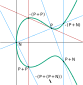
\includegraphics[width=0.48\textwidth]{curve6-doublewithN.pdf}%
    }
\end{center}
\caption{\label{fig:curve5-double}Point doubling, without and with the help of the point $N$.}
\end{figure}

A further trick will help: instead of working with points in $E[r]$, we
will work with points which are \emph{not} in $E[r]$; we will define our
group law as $(P+N)*(Q+N) = (P+Q)+N$. This is equivalent to saying that
we \emph{represent} point $P \in E[r]$ by point $P+N$; we are still
conceptually working with points on the prime order group $E[r]$, but
through their dual points. This small transform has the nice side-effect
of making $N$ the neutral point in the group, i.e. a point with
well-defined $x$ and $y$ coordinates. This will help in making
\emph{complete} formulas, that handle the neutral just like any other
point.

It remains to be seen whether all this leads to efficient formulas. As
will be described in the rest of this document, it does.

\subsection{Summary of Results}

We summarize here the results which will be explained at length in the
remaining pages:
\begin{itemize}

    \item Double-odd elliptic curves are exactly (up to isomorphism)
    curves of equation:
    \begin{equation*}
        y^2 = x(x^2 + ax + b)
    \end{equation*}
    where $a$ and $b$ are two field elements such that neither $b$ nor
    $a^2 - 4b$ is a quadratic residue. This is a large class; about
    1/4th of all curves are double-odd curves (this is similar to, for
    instance, Montgomery curves).

    \item A group of order $r$ is defined as
    $\bG = \{ P+N \,|\, P \in E[r] \}$. The group is homomorphic to the
    curve subgroup of points of $r$-torsion; its neutral element is
    $N = (0, 0)$. Addition in $\bG$ of $P+N$ and $Q+N$ is performed as:
    \begin{equation*}
        (P + N) * (Q + N) = P + (Q + N)
    \end{equation*}

    \item Group element $(x, y)$ is canonically encoded as the value
    $w = y/x$ (value zero for the neutral $N$). A group with $n$-bit
    security is encoded over $2n+1$ bits, which is about the best that
    can be hoped for with elliptic curves, and matches what can be
    achieved with prime order short Weierstraß curves. Decoding is
    intrinsically verified; invalid encodings can be reliably detected
    and rejected. When decoded, the obtained element is necessarily in
    the right prime order group.

    \item Several coordinate systems can be used. We define $(x, w)$ and
    $(x, u)$ systems (with $w = y/x$ and $u = x/y$). With $(x, w)$, we
    get unified formulas (that can be implemented in complete
    \emph{routines}); in $(x, u)$ coordinates, we achieve complete
    formulas.

    \item With Jacobian $(x, w)$ coordinates, we represent points in
    $\bG$ as triplets $(X{:}W{:}Z)$ such that $x = X/Z^2$ and $w = W/Z$.
    These coordinates lead to unified addition formulas with cost 8M+6S,
    and complete doubling formulas with cost 2M+5S (generically on all
    curves) that can be reduced to 1M+6S or even 2M+4S on some curves.
    Moreover, in sequences of successive doublings, marginal cost per
    doubling is 4M+2S for half of double-odd elliptic curves, and as low
    as 2M+4S or even 1M+5S for some curves (a sequence of $n$ doublings
    on these last curves can be done in cost 1S+$n$(1M+5S)). This
    doubling cost is lower than the fastest known doublings on twisted
    Edwards curves.

    \item With fractional $(x, u)$ coordinates, we represent points in
    $\bG$ as quadruplets $(X{:}Z{:}U{:}T)$ such that $x = X/Z$ and
    $u = U/T$. With this representation, generic point addition cost is
    10M, with complete formulas (for mixed addition, with one operand
    in affine $(x, u)$ coordinates, cost is 8M). Doubling cost is 3M+6S.
    Just like in Jacobian $(x, w)$ coordinates, sequences of successive
    doublings can be done with a low per-doubling marginal cost (on
    some curves, cost of $n$ doublings is 3M+$n$(1M+5S)).

    \item Last but not least, the family of double-odd curves includes
    the GLV curves $y^2 = x^3 + bx$ (in a field $\bF_q$ with $q = 1\bmod
    4$), which have been described in 2001\cite{GalLamVan2001}. Such
    curves are precisely those for which we achieve the lowest
    per-doubling cost (1M+5S), and they also feature an efficient
    endomorphism that can be used to further speed up point
    multiplication by a scalar\footnote{This optimization method has
    long been rumoured to be patented, but it seems that the relevant
    patents have expired in September 2020; see discussion in
    section~\ref{sec:curveparams:do255s}.}.

\end{itemize}

Following these results, we define and implement two curves (called
do255e and do255s) that operate over 255-bit fields (integers modulo
$2^{255}-18651$ and $2^{255}-3957$, respectively) and offer the usual
``128-bit'' security level\footnote{Technically, they have only 127-bit
security level, but that's still more than the 126 bits from
Curve25519.}. Curve do255e is a GLV curve; curve do255s is an ordinary
curve with no fast endomorphism. On 64-bit x86 systems (Coffee Lake core),
with curve do255e, we get generic point multiplication in less than
77k cycles (fully constant-time). This translates to the following
performance for high-level operations:
\begin{itemize}
    \item Key pair generation: 49122 cycles (including public key
    encoding into 32 bytes).
    \item Key exchange: 105340 cycles (this is a multiplication of the
    point from the peer by our private key; this cost includes the 18220
    cycles for the decoding of the peer's point from its compact 32-byte
    representation, and the key derivation process with SHAKE256).
    \item Signature generation: 53584 cycles.
    \item Signature verification: 111900 cycles on average (including
    the 18220 cycles for decoding the public key from its compact
    32-byte encoding).
\end{itemize}
We also implement our curves in ARMv6-M assembly (for the Cortex M0+),
and obtain the following:
\begin{itemize}
    \item Key pair generation: 1.42m cycles\footnote{We are using ``m''
    to denote one million.}.
    \item Key exchange: 2.62m cycles.
    \item Signature generation: 1.50m cycles.
    \item Signature verification: 3.26m cycles (average).
\end{itemize}
These performance figures compare favourably to other existing fast
curves. For instance, with Curve25519 on ARM Cortex M0+, the fastest
reported key exchange has cost 3.23m cycles\cite{Por2020-4}.

We also support a constant-time hash-to-curve process, by using a
mapping function, applied twice (two 32-byte chunks are derived from the
input with a suitable hash function, each chunk is mapped to a curve
point, and the two points are added together). Most double-odd elliptic
curves can use Elligator2\cite{BerHamKraLan2013}, which is efficient.
For GLV curves with $a = 0$, Elligator2 is not applicable; we instead
describe a novel map function applicable to such curves.

\subsection{Article Outline}

In the next section (section~\ref{sec:structure}), we study the
structure of double-odd elliptic curves; in particular, we establish
their equation and formally define the prime order group $\bG$.

In section~\ref{sec:formulas}, we establish several formulas for
computing the group law in various affine coordinate systems that apply
to double-odd elliptic curve. We also show that double-odd elliptic
curves can be viewed as a subgroup of a twisted Edwards curve in a
degree-2 field extension, and we describe some isogenies which are
useful in deriving fast formulas for computing point doublings. We
finally describe two maps from arbitrary field elements to curve points
(one is Elligator2, the other is a new map applicable to GLV curves with
equation $y^2 = x(x^2 + b)$).

Section~\ref{sec:algorithms} details the application of these formulas
in several fractional coordinate systems, which allow computations to
proceed with only multiplications but no division (except a single one,
at the end, when encoding a point into bytes). These algorithms
represent the template for practical implementations.

Specific parameter sets for curves do255e and do255s are defined in
section~\ref{sec:curveparams}. The criteria which led to these specific
choices are explained. We also provide in this section a succinct
specification of key exchange and signature algorithms using these
curves.

Implementation details and issues are covered in
section~\ref{sec:implementations}. There we describe our implementation
techniques for both 64-bit x86 (C code with intrinsics and some inline
assembly) and ARM Cortex M0+ (mostly assembly code).

% ----------------------------------------------------------------------

\section{Structure of Double-Odd Elliptic Curves}\label{sec:structure}

\subsection{Notations}\label{sec:structure:notations}

In all the subsequent analysis, we will work in the finite field $\bF_q$
of cardinal $q = p^m$ for a prime $p \geq 5$ (the field characteristic)
and integer $m\geq 1$. Integer constants such as $4$ or $27$ are to be
understood as elements of $\bF_q$ when appropriate (all such constants
will be products of powers of $2$ and $3$ only, therefore non-zero in
$\bF_q$).

$\QR(K)$ is the set of quadratic residues in field $K$: $\QR(K) = \{ x^2
\,|\, x \in K \} $. Note that $0 \in \QR(K)$. Most of the time, we will
work with the field $\bF_q$ and will use the shorthand $QR$ to designate
$QR(\bF_q)$.

$x$, $y$, $u$, $w$... designate point coordinates, i.e. elements of
$\bF_q$. In this section, $X$ is the symbolic identifier for the
generator of the ring of polynomials $\bF_q[X]$, which is used for some
of the demonstrations (in some other later sections, $X$ will be used
to denote some point coordinates in various projective representations;
the context should make it clear).

\subsection{Curve Characterization}\label{sec:structure:characterization}

In this section, we characterize the set of curves over $\bF_q$, with
order $2r$ for an odd integer $r$.

All elliptic curves on $\bF_q$ can be transformed through changes of
variables into a \emph{short Weierstraß} curve, i.e. the set of points
$(x, y) \in \bF_q\times\bF_q$ such that:
    $$ y^2 = x^3 + Ax + B $$
for two given constants $A$ and $B$ in $\bF_q$. The curve also includes
an extra ``point-at-infinity'' which we will denote $\neutral$; that
point does not have $x$ and $y$ coordinates. The curve is an Abelian
group with the following addition law:
\begin{itemize}

    \item The neutral element is $\neutral$.

    \item The opposite of $P = (x, y)$ is $-P = (x, -y)$.

    \item For any two points $P_1$ and $P_2$ such that $P_1 \neq
    \neutral$, $P_2 \neq \neutral$ and $P_1 \neq -P_2$, the line going
    through $P_1$ and $P_2$ will intersect the curve on a third point,
    which is $-(P_1+P_2)$. When $P_1 = P_2$, the line to consider is
    the tangent to the curve on $P_1$.

\end{itemize}
When adding point $P_1 = (x_1, y_1)$ to $P_2 = (x_2, y_2)$, the slope of
the line from $P_1$ to $P_2$ can be computed as $\lambda = (y_2 - y_1) /
(x_2 - x_1)$. If $P_1 = P_2$, this expression is not usable; instead, we
use the tangent, whose slope is $\lambda = (3x^2 + A) / 2y$.

The three following properties are equivalent to each other:
\begin{itemize}

    \item There is no point $(x, y)$ on the curve such that both
    $3x^2 + A = 0$ and $2y = 0$.

    \item $4A^3 + 27B^2 \neq 0$.

    \item The polynomial $X^3 + AX + B \in \bF_q[X]$ does not have a
    multiple root (i.e. it is relatively prime to its derivative
    $3X^2 + A$).

\end{itemize}
If these properties are met, then the law is well-defined and imbues the
curve with an Abelian group structure.

We now want to study double-odd curves, i.e. curves whose order is equal
to $2r$ for an odd integer $r$. The fundamental theorem of finitely
generated Abelian groups\footnote{The history of the discovery and proof
of this theorem is complicated, especially since it predates the formal
definition of groups. Here, we use the sub-case of finite groups, for
which the theorem was proven by Kronecker\cite{Kro1870}.} states that
any finite Abelian group is homomorphic to:
$$ \bZ_{n_1} \times \bZ_{n_2} \times ... \times \bZ_{n_k} $$
for some integers $n_i$ such that $n_i$ divides $n_{i+1}$ for all
$i$ in $1$ to $k-1$. This implies that:
\begin{itemize}

    \item Any Abelian group with an even order must have at least one
    element of order $2$ (if the product of all $n_i$ is even, then at
    least one of them is even).

    \item Any Abelian group whose order is a multiple of $4$ must
    include at least one element of order $4$, or at least three
    elements of order $2$ (if the product of all $n_i$ is a multiple
    of $4$, and $n_k = 2\bmod 4$, then $n_{k-1}$ must be even as
    well).

\end{itemize}
Therefore, curves with order $2r = 2 \bmod 4$ are the curves which
contain a single element of order $2$, and no element of order $4$.
Elements of order $2$ are points $(u, 0)$ for some integer $u$ which
is a root of $X^3 + AX + B$. We can then write:
    $$ X^3 + AX + B = (X - u) (X^2 + uX + (A + u^2)) $$
We will now apply the change of variable $x \mapsto x + u$; this is an
isomorphism between curves, since it preserves lines (straight lines are
mapped to straight lines) and therefore also preserves the structure
induced by the group law. This turns the curve equation into:
    $$ y^2 = x (x^2 + ax + b) $$
for constants $a$ and $b$ such that:
\begin{align*}
    a &= 3u \\
    b &= A + 3u^2
\end{align*}
From now on, we will consider curves using this alternate equation.
Conversely, any curve using that equation can be turned back into a
short Weierstraß equation by applying the $x \mapsto x - a/3$
change of variable, yielding:
\begin{align*}
    A &= (3b - a^2) / 3 \\
    B &= a(2a^2 - 9b) / 27
\end{align*}
The curve is well-defined if and only if there is no double root to
the polynomial $X^3 + aX^2 + bX$, i.e. if and only if the two following
properties hold:
\begin{itemize}

    \item $b \neq 0$ (otherwise, $0$ would be a double root).

    \item $a^2 - 4b \neq 0$ (otherwise, $X^2+aX+B$ would have a
    double root).

\end{itemize}

The point $N = (0, 0)$ is part of the curve, and has order $2$. This is,
by construction, the only point with $x = 0$. As will be detailed below
(section~\ref{sec:structure:coreformulas}), for any point $P = (x,y)$ with
$x, y \neq 0$, the point $P+N$ has coordinates $(b/x, -by/x^2)$.

For the curve to have order $2r = 2 \bmod 4$, $N$ must be the only
point of order $2$, i.e. there should be no other root to $X^3+aX^2+bX$.
This implies that $a^2 - 4b \notin \QR$. Moreover, if $b \in \QR$, then
let $c$ be a square root of $b$; in that case:
    $$ a^2 - 4b = (a + 2c)(a - 2c) $$
Since $a^2 - 4b \notin \QR$, then one of $a+2c$ and $a-2c$ must be a
quadratic residue. Without loss of generality, suppose that $a+2c \in
\QR$. Then, points $(\pm c, \pm c\sqrt{a+2c})$ are on the curve, and
have order $4$: each such point $P$ is such that $P+N = -P$. Therefore,
a curve of order $2r = 2\bmod 4$ must have $b \notin \QR$.

Conversely, consider a curve with equation $y^2 = x(x^2 + ax + b)$ for any
$a, b \in \bF_q$ such that $b \neq 0$ and $a^2 - 4b \neq 0$. Such a
curve contains the point $N = (0, 0)$, and thus its order is even. If its
order is a multiple of $4$, then either:
\begin{itemize}

    \item there is at least another point of order $2$, which
    implies that $X^2+aX+b$ has roots in $\bF_q$, and therefore
    $a^2 - 4b \in \QR$; or

    \item the curve contains a point $Q = (x_4, y_4)$ of order $4$
    such that $2Q = N$, which means that $Q+N = -Q$, which implies that
    $x_4 = b/x_4$, and thus $b \in \QR$.

\end{itemize}

All these facts can be summarized into the following:

\vspace{2ex}
\noindent\fbox{\begin{minipage}{\textwidth - 6.8pt}
\begin{center}\textsf{\textbf{Characterization of double-odd elliptic curves:}}\end{center}
Elliptic curves $E$, over a finite field $\bF_q$ of characteristic
$p\geq 5$, and whose order is equal to $2$ modulo $4$, are exactly, up
to isomorphisms, the curves with equation:
    $$ y^2 = x(x^2 + ax + b) $$
for two constants $a, b \in \bF_q$ such that:
\begin{itemize}
    \item $a^2 - 4b$ is not a quadratic residue;
    \item $b$ is not a quadratic residue.
\end{itemize}
\end{minipage}}

\subsection{Core Addition Formulas}\label{sec:structure:coreformulas}

Let $P_1 = (x_1, y_1)$ and $P_2 = (x_2, y_2)$ two points on a curve $E$
of equation $y^2 = x(x^2 + ax + b)$; neither point is the special
point-at-infinity ($\neutral$) since that point does not have coordinates.
Let $P_3 = P_1 + P_2$. The coordinates $(x_3, y_3)$ of $P_3$ can be
obtained as follows:
\begin{itemize}

    \item If $x_1 = x_2$ and $y_1 = -y_2$, then $P_3 = \neutral$ (with
    no defined coordinates).

    \item Otherwise, if $x_1 = x_2$, then $y_1 = y_2$ and $P_1 = P_2$;
    define the slope of the tangent to the curve on $P_1$ as:
    \begin{equation*}
        \lambda = \frac{3x_1^2 + 2ax_1 + b}{2y_1}
    \end{equation*}
    and the coordinates of $P_3$ are:
    \begin{align*}
        x_3 &= \lambda^2 - a - 2x_1 \\
        y_3 &= \lambda(x_1 - x_3) - y_1
    \end{align*}

    \item Otherwise, $x_1 \neq x_2$, and we can compute the slope
    $\lambda$ of the line from $P_1$ to $P_2$ as:
    \begin{equation*}
        \lambda = \frac{y_2 - y_1}{x_2 - x_1}
    \end{equation*}
    and the coordinates of $P_3$ are:
    \begin{align*}
        x_3 &= \lambda^2 - a - x_1 - x_2 \\
        y_3 &= \lambda(x_1 - x_3) - y_1
    \end{align*}

\end{itemize}

From these formulas, we now consider two important sub-cases. The
first one is when adding a point $P = (x, y)$ to $N = (0, 0)$ (the
point of order 2). If $P \neq N$, then $x \neq 0$ and the slope
of the line $(PN)$ is:
\begin{equation*}
    \lambda = \frac{y}{x}
\end{equation*}
yielding the coordinates $(x', y')$ of $P' = P + N$:
\begin{align*}
    x' &= \frac{y^2}{x^2} - a - x \\
       &= \frac{x^3 + ax^2 + bx - ax^2 - x^3}{x^2} \\
       &= \frac{b}{x} \\[2ex]
    y' &= \frac{y}{x}\left(x - \frac{b}{x}\right) - y \\
       &= -\frac{by}{x^2}
\end{align*}

The second sub-case is that of point doubling, i.e. adding a point to
itself. Let $P = (x, y) \neq N$, and $P_2 = 2P$. The coordinate $x$
of $P_2$ is computed as:
\begin{align*}
    x_2 =&\ \left(\frac{3x^2 + 2ax + b}{2y}\right)^2 - a - 2x \\
    =&\ \frac{9x^4 + 12ax^3 + (4a^2+6b)x^2 + 4abx + b^2}{(2y)^2} \\
     &\  - \frac{4ax^3 - 4a^2x^2 - 4abx}{(2y)^2}
        - \frac{8x^4 - 8ax^3 - 8bx^2}{(2y)^2} \\
    =&\ \frac{x^4 - 2bx^2 + b^2}{(2y)^2} \\
    =&\ \left(\frac{x^2-b}{2y}\right)^2
\end{align*}
Therefore, the $x$ coordinate of $2P$, for any point $P \neq \neutral,N$,
is a quadratic residue.

\subsection{A Prime Order Group}\label{sec:structure:groupdef}

Let $E$ be a curve of order $2r = 2 \bmod 4$; $r$ is an odd integer. We
will now define a group of order $r$, homomorphic to a subgroup of size
$r$ in $E$, with a canonical encoding as field elements. All the
analysis here works for any odd integer $r$, but most cryptographic
applications (e.g. signatures) will require $r$ to be prime; we then
assume that the curve parameters ($\bF_q$, $a$ and $b$) are chosen so
that $r$ is a prime of appropriate length.

Let $E[r]$ be the set of points of $r$-torsion in $E$, i.e. the points
which, multiplied by $r$, yield $\neutral$. This is a subgroup of $E$.
In fact, any point on $E$ can be decomposed into a sum of two
points $P_r + P_t$, where $P_r \in E[r]$ and $P_t \in \{ \neutral, N \}$;
points $P_r$ and $P_t$ can be computed as:
\begin{align*}
    P_r &= (r + 1)P \\
    P_t &= rP
\end{align*}
This decomposition is unique. Note that $N \notin E[r]$.

Suppose that $P = (x, y) \in E[r]$ and $P \neq \neutral$; consider the
line that goes from $N$ to $P$. Since $N$ is the only point on the curve
with $x = 0$, and also the only point on the curve with $y = 0$, the
line $(PN)$ has a defined non-zero slope $w = y/x$. This line, by
construction, intersects the curve at a third point which is $-P+N$. In
particular, $-P+N \notin E[r]$. Similarly, if we had started from $P'
\notin E[r]$ and $P' \neq N$, then the line $(P'N)$ has slope $w' =
y'/x'$ and intersects the curve on a third point, which is $-P'+N$, and
which is part of $E[r]$. Thus, any given slope $w\neq 0$ may correspond
to only two points on the curve, exactly one of which is in $E[r]$.

If $P \in E[r]$, then $P = P_r = (r+1)P = 2((r+1)/2)P$: every point in
$E[r]$ is the double of some other point. As we saw in
section~\ref{sec:structure:coreformulas}, this implies that the $x$
coordinate of any point $P \in E[r]$ ($P \neq \neutral$) is a quadratic
residue. Conversely, for any point $P' = (x', y') \notin E[r]$ (and
$P' \neq N$), we saw that $P' = P + N$ with $x' = b/x$, for some point
$P$ which will then be a point of $r$-torsion. Thus, $x \in \QR$. Since
$b \notin \QR$, it follows that $x' \notin \QR$. These properties lead
to the following important fact:

\vspace{2ex}
\noindent\fbox{\begin{minipage}{\textwidth - 6.8pt}
\begin{center}\textsf{\textbf{Characterization of \emph{r}-torsion points}}\end{center}
For any point $P = (x, y) \in E$ such that $P\neq \neutral, N$,
$P \in E[r]$ if and only if $x \in QR$.
\end{minipage}}

\vspace{2ex}
We will now define a group of order $r$ whose elements can be uniquely
encoded to, and decoded from, field elements. The group will be
homomorphic to $E[r]$, but we choose to represent elements by points
which are \emph{not} in $E[r]$ for reasons which will be explained
below. Here is the group definition:

\vspace{2ex}
\noindent\fbox{\begin{minipage}{\textwidth - 6.8pt}
\begin{center}\textsf{\textbf{Group of odd order \emph{r}}}\end{center}
Elements of $\bG$ are the curve points which are not in $E[r]$:
\begin{equation*}
    \bG = \{ P+N \,|\, P \in E[r] \}
\end{equation*}
These are exactly the points of $E$ whose $x$ coordinate is either $0$
(for point $N$) or not a quadratic residue in $\bF_q$.

For $P_1+N$ and $P_2+N$ in $\bG$, the group law yields:
\begin{equation*}
    (P_1 + N) * (P_2 + N) = (P_1 + P_2) + N
\end{equation*}
The neutral point is $N$. The opposite of $P_1+N$ is
$-P_1+N = -(P_1+N)$.
\end{minipage}}

\vspace{2ex}
Elements of $\bG$ can be encoded into field elements with the following
map:
\begin{equation*}
    \begin{array}{rrcll}
        \phi : & \bG &\longrightarrow & \bF_q & \\
        & (P_1 + N) &\longmapsto & 0 & \text{\ \ \ if\ } (P_1 + N) = N \\
        & & & y/x & \text{\ \ \ if\ } (P_1 + N) = (x, y) \neq N
    \end{array}
\end{equation*}
As we saw above, this map is injective: any value $w = y/x \neq 0$
corresponds to only two points on the curve, only one of which being in
$\bG$. The decoding process, from a given $w \in \bF_q$, is as follows:
\begin{itemize}

    \item If $w = 0$, then the point is $N$.

    \item Otherwise, consider the equation $x^2 - (w^2 - a)x + b = 0$
    (this is a rewriting of the curve equation, replacing $y$ with $wx$,
    and dividing by $x$). This is a quadratic equation in $x$, whose
    discriminant is $\Delta = (w^2 - a)^2 - 4b$; note that $\Delta \neq
    0$ (otherwise, it would imply that $b \in \QR$). If $\Delta \notin
    \QR$, then there is no solution (the provided $w$ is not the image
    of a group element by $\phi$); otherwise, there are two distinct
    solutions:
    \begin{equation*}
        x = \frac{w^2 - a \pm \sqrt{\Delta}}{2}
    \end{equation*}
    The two solutions are such that their product is $b$, which is not a
    quadratic residue; thus, exactly one of the solutions is not a
    quadratic residue: this is the $x$ coordinate of the point $P+N$
    such that $\phi(P+N) = w$. The $y$ coordinate of $P+N$ is obtained
    as: $y = xw$.

\end{itemize}

We could have defined $\bG$ to be $E[r]$, using point addition as group
law, and with the same mapping to field elements (decoding would then have
chosen the solution $x$ which is a quadratic residue). However, we
prefer the formulation above for the following reasons:
\begin{itemize}

    \item Every element of $\bG$ has defined $(x,y)$ coordinates. The
    neutral element is $N = (0,0)$; the curve point-at-infinity $\neutral$
    is not in $\bG$.

    \item The group law can be computed as:
    \begin{equation*}
        (P_1 + N) * (P_2 + N) = (P_1 + P_2) + N = P_1 + (P_2 + N)
    \end{equation*}
    Notice that $P_1 \in E[r]$ but $P_2 + N \notin E[r]$. Therefore, it
    cannot happen that $P_1 = P_2 + N$. This means that addition
    formulas can be applied without encountering the special case of
    adding a point to itself. This will help in establishing unified and
    complete formulas, as will be detailed in section~\ref{sec:formulas}.

\end{itemize}

\subsection{Curve Isomorphisms}\label{sec:structure:isomorphism}

For any non-zero value $\varepsilon$ in $\bF_q$, the mapping
$(x,y) \mapsto (x',y') = (x\varepsilon^2, y\varepsilon^3)$ is an isomorphism
from curve $y^2 = x(x^2+ax+b)$ to curve
$y'^2 = x'(x'^2 + (a\varepsilon^2)x' + (b\varepsilon^4))$ (this is the usual
isomorphism on Weierstraß curves, applied to our curve equation).

The \emph{$j$-invariant} of an elliptic curve is a quantity which is
conserved by such isomorphisms. For a short Weierstraß curve
$y^2 = x^3 + Ax + B$, the $j$-invariant is defined as:
    $$ j = 1728 \frac{4A^3}{4A^3 + 27B^2} $$
In our case, for curves $y^2 = x(x^2 + ax + b)$, we obtain:
    $$ j = \frac{256 (3b - a^2)^3}{b^2(4b - a^2)} $$

When $j \neq 0$ and $j\neq 1728$, there are exactly two curves (up to
isomorphism) that have this $j$-invariant, and they are quadratic twists
of each other (i.e. they become the same curve when lifted into the
extension field $\bF_{q^2}$). For curve $y^2 = x(x^2 + ax + b)$, the
quadratic twist has equation $y^2 = x(x^2 - ax + b)$. If a curve has
order $2r$, then its twist has order $2q + 2 - 2r$, which is then also
equal to $2$ modulo $4$.

The case $j = 0$ is not very interesting to us. Indeed, such a curve is
isomorphic to the short Weierstraß curve $y^2 = x^3 + B$ for some $B\neq
0$. If $q = 1 \bmod 3$, then such a curve has either no point of order
$2$, or three distinct points of order $2$; in both cases, the curve
order cannot be equal to $2$ modulo $4$. If $q = 2 \bmod 3$, the curve
is supersingular with order exactly $q+1$; this can be equal to $2$
modulo $4$ if $q = 1 \bmod 4$ (which, combined with $q = 2 \bmod 3$,
implies $q = 5 \bmod 12$). However, such a supersingular curve has
embedding degree $2$: the Weil pairing maps discrete logarithm on the
curve into the discrete logarithm problem on the multiplicative subgroup
of $\bF_{q^2}$, for which sub-exponential algorithms are
known\cite{MenOkaVan1993}. In order to obtain a decent level of
security, one would have to make $q$ quite large (at least 1024 bits),
implying poor computing performance and large values.

Curves with $j = 1728$ are more useful: this situation is obtained with
$a = 0$. Note that the condition $a^2 - 4b \notin \QR$ then implies that
$-b \notin \QR$. Since we also need $b \notin \QR$, a curve of order $2$
modulo $4$ can have $j = 1728$ only if $q = 1\bmod 4$ (indeed, if $q =
3\bmod 4$, then the curve would be supersingular and its order would be
a multiple of $4$). A non-supersingular curve with $j = 1728$ admits one
quadratic twist and two quartic twists that share the same
$j$-invariant; if $\zeta$ is a non-quadratic residue in $\bF_q$, then
the twists of curve $y^2 = x(x^2 + b)$ can be obtained as:
\begin{itemize}

    \item quadratic twist: $y^2 = x(x^2 + b\zeta^2)$

    \item quartic twists: $y^2 = x(x^2 + b\zeta)$ and
    $y^2 = x(x^2 + b\zeta^3)$

\end{itemize}
This works from any $\zeta \notin \QR$, in particular $\zeta = b$. Note
that if $b \notin \QR$, then $b\zeta$ and $b\zeta^3$ are quadratic
residues, which means that the quartic twists are \emph{not} curves
with order 2 modulo 4.

Curves with $j = 1728$ are a type of GLV curve\cite{GalLamVan2001}: the
map $(x, y) \mapsto (-x, \eta y)$, for $\eta$ a primitive 4-th root of
unity in $\bF_q$, can be very efficiently computed, and it is an
endomorphism of the curve, corresponding to multiplication of the point
by a certain constant $\mu$. This endomorphism can be used to speed up
point multiplication; this will be explained in more details in
section~\ref{sec:implementations:glv}.

% ----------------------------------------------------------------------

\section{Formulas}\label{sec:formulas}

In this section, we derive several addition formulas for our group
$\bG$, defined in section~\ref{sec:structure:groupdef}, using various
representations of coordinates. We still stick to ``affine''
coordinates; practical implementations would rather use one of the
fractional systems which will be detailed in
section~\ref{sec:algorithms}. Thus, this section is still concerned with
laying out mathematical foundations.

We use the following conventions:
\begin{itemize}

    \item Group element $P_1+N$ has coordinates $(x_1,y_1)$. Take care
    that $(x_1,y_1)$ are the coordinates of $P_1+N$, not of $P_1$.

    \item We seek formulas to compute the coordinates $(x_3,y_3)$ of
    point $P_3+N$, which is equal to $(P_1+N)*(P_2+N)$.

    \item When explicitly considering element doubling (applying the
    law on a point and itself), the point $P+N$ has coordinates $(x,y)$,
    and its double $2P+N$ has coordinates $(x',y')$.

\end{itemize}

The group law in $\bG$ is denoted with the ``$*$'' operator; in the rest
of the article, we will call it ``addition in $\bG$''. Conversely, in the
few instances where we refer to the traditional addition of curve points,
we will use the expression ``addition on the curve''.

\subsection{On Formula Completeness}\label{sec:formulas:completeness}

In all generality, formulas that work for most input points may have
exceptional cases, for which they do not return the right result.
Following the terminology in \cite{BerLan2007}, we will say that:
\begin{itemize}

    \item Formulas with no exceptional case are \emph{complete}.

    \item Formulas whose only exceptional cases are such that one of the
    input points, or the output point, is the group neutral element
    ($N$), are \emph{unified}.

\end{itemize}

On standard Weierstraß curves, with affine $(x,y)$ coordinates, the
formulas for adding two points together are neither complete nor
unified, since they must make a special case for adding a point to
itself. Thanks to our definition of the group $\bG$ and its law, we will
naturally avoid such issues, since we compute the addition of $P_1+N$
and $P_2+N$ in $\bG$ as the addition on the curve of points $P_1$ and
$P_2+N$; these two points are always distinct since $P_1 \in E[r]$ but
$P_2+N \notin E[r]$. All our formulas are thus always unified, and we
will see that some of them are complete.

Non-unified formulas can be a problem for secure implementation: correct
handling of exceptional cases will imply either side channels (some of
the code will be executed conditionally, depending on the input points)
or substantial execution overhead (the general and the exceptional cases
being both executed systematically). In some cases, it can be shown that
operations cannot be exceptional. For instance, suppose that a routine
multiplies a given curve point by a scalar, the point being part of a
curve of prime order and different from the point-at-infinity, and the
scalar being non-zero and lower than the curve order (this is the
classic situation of a Diffie-Hellman key exchange). In that situation,
a classic double-and-add algorithm will involve explicit doublings, and
extra additions; it can be shown that none of the extra additions can be
a doubling, and therefore a routine that cannot handle that exceptional
case is usable. However, most implementations of point multiplications
will improve the double-and-add algorithm with window optimizations, and
will furthermore apply Booth recoding on the scalar\cite{Boo1951} to
reduce the size of the individual digits; in that case, it is no longer
true that all point additions are exception-less. More generally, this
kind of analysis depends on how the point addition is used, and cannot
necessarily be extended to all protocols.

Unified formulas avoid most of these issues. A complete \emph{routine}
can be made out of unified formulas, by handling the remaining
exceptional cases with a pair of constant-time conditional copy
operations (adding an element with the neutral element should yield back
the first element). Using complete \emph{formulas} can avoid even such
conditional copies. Generally speaking, complete routines are
sufficient for most secure implementations; complete formulas are
helpful in some specific contexts, such as the following:
\begin{itemize}

    \item Some hardware platforms may provide efficient accelerators
    for arithmetic operations on field elements, but not for making
    efficient constant-time comparisons and conditional copies.

    \item In some homomorphic encryption or zero-knowledge proof
    systems, coordinates are not directly accessible, but manipulated
    through a blinding layer that allows arithmetic operations on field
    elements, but not constant-time conditional copies.

\end{itemize}

Additionally, in some cases, formulas which are only unified with affine
coordinates become complete when used with some fractional coordinate
systems, leading to complete algorithms (and implementations). Some such
examples will be seen in section~\ref{sec:algorithms}.

\subsection{Affine \emph{(x, y)} Coordinates}\label{sec:formulas:xy}

Let $P_1+N = (x_1,y_1)$, $P_2+N = (x_2,y_2)$, and their sum (in $\bG$)
$P_3+N = (x_3,y_3)$. We first suppose that neither $P_1+N$ nor $P_2+N$
is the neutral element $N$; thus, $x_1$, $y_1$, $x_2$ and $y_2$ are
non-zero. The curve point $P_2$ has coordinates $(b/x_2, -by_2/x_2^2)$.
The slope of the line from $P_1+N$ to $P_2$ is:
\begin{align*}
    \lambda &= \frac{\frac{-by_2}{x_2^2} - y_1}{\frac{b}{x_2} - x_1} \\
    &= \frac{x_1 x_2^2 y_1 + b x_1 y_2}{x_1 x_2 (x_1 x_2 - b)}
\end{align*}
The coordinates of $P_3+N$ are then:
\begin{align*}
    x_3 &= \lambda^2 - a - x_1 - \frac{b}{x_2} \\
    y_3 &= \lambda (x_1 - x_3) - y_1
\end{align*}
Applying the expression of $\lambda$ above, and simplifying (replacing
$y_1^2 = x_1^3 + ax_1^2 + bx_1$, and similarly for $y_2^2$, and taking
into account that $x_1 x_2 \neq 0$), yields the following formulas:

\vspace{2ex}
\noindent\fbox{\begin{minipage}{\textwidth - 6.8pt}
\begin{center}\textsf{\textbf{Addition in $\bG$}} ($(x, y)$ coordinates, complete)\end{center}
\vspace{-2ex}
\begin{align*}
    x_3 &= \frac{b((x_1 + x_2)(x_1 x_2 + b) + 2a x_1 x_2 + 2 y_1 y_2)}{(x_1 x_2 - b)^2} \\
    y_3 &= \frac{b(2a(x_1 y_2 + x_2 y_1)(x_1 x_2 + b) + (x_1^2 y_2 + x_2^2 y_1)(x_1 x_2 + 3b) + (y_1 + y_2)(3b x_1 x_2 + b^2))}{-(x_1 x_2 - b)^3}
\end{align*}
\end{minipage}}

\vspace{2ex}
These formulas are complete: they are unified by construction, and it is
easily seen that if $(x_1,y_1) = (0,0)$ or $(x_2,y_2) = (0,0)$, the
correct result is obtained.

Noticing that:
\begin{equation*}
    \frac{(y_1 x_2 + y_2 x_1)^2}{x_1 x_2} = (x_1 + x_2)(x_1 x_2 + b) + 2a x_1 x_2 + 2 y_1 y_2
\end{equation*}
and that:
{\setlength\multlinegap{0pt}%
\begin{multline*}
    (y_1 x_2 + y_2 x_1)((y_1 y_2 + a x_1 x_2)(x_1 x_2 + b) + 2b x_1 x_2 (x_1 + x2)) = \\
    x_1 x_2 (2a(x_1 y_2 + x_2 y_1)(x_1 x_2 + b) + (x_1^2 y_2 + x_2^2 y_1)(x_1 x_2 + 3b) + (y_1 + y_2)(3b x_1 x_2 + b^2))
\end{multline*}}
we can simplify the formulas into:
\begin{align*}
    x_3 &= \frac{b(y_1 x_2 + y_2 x_1)^2}{x_1 x_2 (x_1 x_2 - b)^2} \\
    y_3 &= \frac{-b (y_1 x_2 + y_2 x_1)((y_1 y_2 + a x_1 x_2)(x_1 x_2 + b) + 2b x_1 x_2 (x_1 + x2))}{x_1 x_2 (x_1 x_2 - b)^3}
\end{align*}
However, these alternate formulas are only unified, not complete, since
setting $x_1 = 0$ or $x_2 = 0$ implies an undefined division by zero.

\subsection{Affine \emph{(x, w)} Coordinates}\label{sec:formulas:xw}

Since group elements are encoded as the ratio $w = y/x$, we may try
to use $w$ itself as a coordinate. In $(x,w)$ coordinates, the curve
equation is:
\begin{equation*}
    w^2 x = x^2 + ax + b
\end{equation*}

The neutral point $N$ cannot be represented in $(x,w)$ coordinates: that
point does not have a defined $w$ coordinate. Therefore, we will not
obtain complete formulas as long as we keep to affine representation (we
may still get complete formulas when switching to fractional
representations, e.g. Jacobian coordinates; this will be investigated in
section~\ref{sec:algorithms:xwJ}).

$(x,w)$ coordinates have a number of properties which are useful for
deriving formulas:
\begin{itemize}

    \item No point with defined $(x,w)$ coordinates has $x = 0$ or $w = 0$.

    \item If point $P \neq \neutral, N$ has coordinates $(x,w)$, then:
    \begin{align*}
        -P &= (x, -w) \\
        P+N &= (b/x, -w) \\
        -P+N &= (b/x, w)
    \end{align*}

    \item If $x \neq 0$, then $x + b/x = w^2 - a$ and $x - b/x = 2x + a - w^2$.

\end{itemize}

We now derive formulas in $(x,w)$ coordinates. We consider two group
elements $P_1+N = (x_1, w_1)$ and $P_2+N = (x_2, w_2)$, and their sum
$P_3+N = (x_3, w_3)$ in the group $\bG$. For now, we assume that $P_1+N
\neq N$, $P_2+N \neq N$, and $P_3+N \neq N$. This implies that $x_1$,
$x_2$, $w_1$, $w_2$ and $w_1 + w_2$ are non-zero. Using the alternate
formulas from the previous section, replacing each $y$ with $xw$ and
simplifying fractions by removing common non-zero factors, we obtain the
following unified formulas (they are not complete since $N$ does not
have a well-defined $w$ coordinate).

\vspace{2ex}
\noindent\fbox{\begin{minipage}{\textwidth - 6.8pt}
\begin{center}\textsf{\textbf{Addition in $\bG$}} ($(x, w)$ coordinates, unified)\end{center}
\vspace{-2ex}
\begin{align*}
    x_3 &= \frac{b x_1 x_2 (w_1 + w_2)^2}{(x_1 x_2 - b)^2} \\
    w_3 &= -\frac{(w_1 w_2 + a)(x_1 x_2 + b) + 2b(x_1 + x_2)}{(w_1 + w_2)(x_1 x_2 - b)}
\end{align*}
\end{minipage}}

\vspace{2ex}
When adding a point to itself, the generic formulas above can be
simplified. Suppose that we want to compute $2P+N = (x',w')$ from
$P+N = (x,w)$; the generic formulas become:
\begin{align*}
    x' &= \frac{4b x^2 w^2}{(x^2-b)^2} \\
    w' &= -\frac{(w^2+a)(x^2+b) + 4bx}{2w(x^2-b)}
\end{align*}
Dividing numerator and denominator in both fractions by $x$, and replacing
$(x^2+b)/x$ and $(x^2-b)/x$ with $w^2-a$ and $2x + a - w^2$, respectively,
yields the following doubling formulas:

\vspace{2ex}
\noindent\fbox{\begin{minipage}{\textwidth - 6.8pt}
\begin{center}\textsf{\textbf{Doubling in $\bG$}} ($(x, w)$ coordinates, unified)\end{center}
\vspace{-2ex}
\begin{align*}
    x' &= \frac{4bw^2}{(2x + a - w^2)^2} \\
    w' &= - \frac{w^4 + (4b-a^2)}{2w(2x + a - w^2)}
\end{align*}
\end{minipage}}

\vspace{2ex}
Note that if $P+N \neq N$, then $2P+N \neq N$, since we work in a group
$\bG$ of odd order. Therefore, the only exceptional case to worry about
for doublings is when the input point is already the neutral point $N$.

\subsection{Mapping to a Twisted Edwards Curve Subgroup}\label{sec:formulas:ed}

Double-odd curves are \emph{not} equivalent to twisted Edwards curves
over the same field, since the order of a twisted Edwards curve is
always a multiple of 4. However, a double-odd curve can be mapped into a
subgroup of a twisted Edwards curve in a field extension of degree 2,
using the formulas described in this section.

Let $i$ such that $i^2 = b$. Since $b \notin \QR$, $i$ cannot exist in
$\bF_q$; therefore, $i$ defines a field extension $\bF_{q^2}$. An
element $v \in \bF_{q^2}$ can be uniquely written as:
\begin{equation*}
    v = \Re(v) + i \Im(v)
\end{equation*}
for two values $\Re(v)$ and $\Im(v)$ in $\bF_q$, which we will call, by
analogy with complex numbers, the ``real part'' and ``imaginary part'' of
the value $v$.

For a point $P = (x, y) \in E$, we define the two coordinates $u$
and $v$ as follows:
\begin{align*}
    u &= \frac{x}{y} \\
    v &= \frac{x-i}{x+i}
\end{align*}
If $P = N$, the fraction $x/y$ is undefined, and we set $u = 0$. In that
case, $v = -1$. If $P = \neutral$, we set $u = 0$ and $v = 1$. Note that:
\begin{itemize}
    \item $u \in \bF_q$ for all points $P \in \bG$; moreover, $u\neq 0$
    when $P \neq N, \neutral$.
    \item $v \notin \bF_q$ except when $P = N$ or $\neutral$, in which case
    $v = \pm 1$.
\end{itemize}
This transformation is reversible; the original $x$ and $y$ can be
recomputed with:
\begin{align*}
    x &= i \frac{1+v}{1-v} \\
    y &= \frac{x}{u}
\end{align*}
(and the mapping to $N$ or $\neutral$ when $v \in \bF_q$.)

Note that if $P \in E$ is mapped to $(u, v)$, then $P+N$ is mapped
to $(-u, -v)$. This is true for all points of $E$, including $N$ and
$\neutral$.

Replacing $x$ and $y$ with their expressions in $u$ and $v$ into the
curve equation $y^2 = x(x^2 + ax + b)$ leads to the following:
\begin{equation*}
    (a + 2i)u^2 + v^2 = 1 + (a - 2i)u^2 v^2
\end{equation*}
which is the equation of a twisted Edwards curve.

Twisted Edwards curves are defined and analyzed in
\cite{BerBirJoyLanPet2008}. If points $P_1$ and $P_2$ have coordinates
$(u_1, v_1)$ and $(u_2, v_2)$, respectively, and $P_1 + P_2$ has
coordinates $(\hat u, \hat v)$, then:
\begin{align*}
    \hat u &= \frac{u_1 v_2 + u_2 v_1}{1 + (a - 2i) u_1 u_2 v_1 v_2} \\
    \hat v &= \frac{v_1 v_2 - (a + 2i) u_1 u_2}{1 - (a - 2i) u_1 u_2 v_1 v_2}
\end{align*}
Take care that we are here talking about point addition, i.e. not the
composition law in our group $\bG$. We will investigate the formulas
for $\bG$ later on.

\cite{BerBirJoyLanPet2008} shows that these formulas are complete
provided that the first curve equation constant (here $a - 2i$) is a
quadratic residue, and the second constant (here $a + 2i$) is not.
However, this is not the case here; indeed, none of the four values $\pm
a\pm 2i$ can be a quadratic residue in $\bF_{q^2}$, because that would
imply that $a^2 - 4b \in \QR(\bF_q)$, which would be incompatible with
our initial curve construction.

We can still show that the formulas, while not necessarily complete
\emph{in general}, are still complete for the subset of points which are
the mapping of points from our original curve $E$. As explained in
\cite{BerBirJoyLanPet2008}, the twisted Edwards curve is isomorphic to a
non-twisted curve by the mapping $u \mapsto u/\sqrt{a - 2i}$; since $a -
2i \notin \QR(\bF_{q^2})$, such a mapping requires lifting the curve
into another field extension, this time into $\bF_{q^4}$. Then, the
demonstration in \cite{BerLan2007} (section 3) applies and shows that
the formulas are correct for all inputs such that the denominators ($1
\pm (a - 2i) u_1 u_2 v_1 v_2$ in our case) are non-zero. Thus, we only
need to prove that there are no points $(x_1, y_1)$ and $(x_2, y_2)$ in
$E$, such that their mappings into coordinates $(u_1, v_1)$ and $(u_2,
v_2)$ would lead to $1 \pm (a - 2i) u_1 u_2 v_1 v_2 = 0$.

First, notice that if $P_1 = N$ or $\neutral$, then $u_1 = 0$ and $1 \pm
(a - 2i) u_1 u_2 v_1 v_2 = 1 \neq 0$. This is also the case if $P_2 = N$
or $\neutral$. We can thus restrict ourselves to the case where $P_1
\neq N, \neutral$ and $P_2 \neq N, \neutral$, i.e. $x_1$, $x_2$, $u_1$
and $u_2$ are non-zero. Replacing $v$ with $(x-i)/(x+i)$, we obtain that:
\begin{align*}
    \Im((a - 2i) u_1 u_2 v_1 v_2) = \frac{-2 u_1 u_2 x_1 x_2}{(x_1^2 - b)(x_2^2 - b)}\left(\frac{1}{u_1^2 u_2^2} - (a^2 - 4b)\right)
\end{align*}
which is non-zero, since $a^2 - 4b \notin \QR(\bF_q)$. Therefore, the
denominators can never be zero for the points mapped from $E$, and the
formulas are complete for these points.

\subsection{Affine \emph{(x, u)} Coordinates}\label{sec:formulas:xu}

We now use the twisted Edwards curve formulas to derive additional
formulas for $\bG$. As previously, we consider two points $P_1+N$ and
$P_2+N$ in $\bG$, and their sum (in $\bG$) $P_3+N = (P_1+N)*(P_2+N)$.
Since this means that $P_3 = (P_1+P_2)+N$, we can use the formulas
above, then apply the $+N$ operation, which, in $(u,v)$ coordinates,
is just negation of the values:
\begin{align*}
    u_3 &= -\frac{u_1 v_2 + u_2 v_1}{1 + (a - 2i) u_1 u_2 v_1 v_2} \\
    v_3 &= -\frac{v_1 v_2 - (a + 2i) u_1 u_2}{1 - (a - 2i) u_1 u_2 v_1 v_2}
\end{align*}
For better performance, we want to work only in $\bF_q$, and thus we need
to use $x$ instead of $v$ as input, and revert to $x$ on output. Applying
the map $v \mapsto x$ into the equation for $v_3$ yields the following
(after multiplying numerator and denominator by $(x_1-i)(x_2-i)$, which
is always non-zero since $x_1, x_2 \in \bF_q$):
\begin{equation*}
    v_3 = -\frac{(x_1 - i)(x_2 - i) - (a + 2i) u_1 u_2 (x_1 + i)(x_2 + i)}
                 {(x_1 + i)(x_2 + i) - (a - 2i) u_1 u_2 (x_1 - i)(x_2 - i)}
\end{equation*}
Developing this expression, then multiplying numerator and denominator by
$i$ and inserting the minus sign in the numerator leads us to:
\begin{equation*}
    v_3 = \frac{C - iD}{C + iD}
\end{equation*}
with:
\begin{align*}
    C &= b((x_1 + x_2)(1 + a u_1 u_2) + 2 u_1 u_2 (x_1 x_2 + b)) \\
    D &= (x_1 x_2 + b)(1 - a u_1 u_2) - 2b u_1 u_2 (x_1 + x_2)
\end{align*}
Since we know that $v_3 = (x_3 - i) / (x_3 + i)$ for some $x_3 \in \bF_q$,
it follows that $x_3 = C/D$.

A similar treatment to the expression of $u_3$ yields:
\begin{equation*}
    u_3 = -\frac{F + iG}{H + iJ}
\end{equation*}
with:
\begin{align*}
    F &= (u_1 + u_2)(x_1 x_2 - b) \\
    G &= (u_1 - u_2)(x_2 - x_1) \\
    H &= (x_1 x_2 + b)(1 + a u_1 u_2) + 2b u_1 u_2 (x_1 + x_2) \\
    J &= (x_1 + x_2)(1 - a u_1 u_2) - 2 u_1 u_2 (x_1 x_2 + b)
\end{align*}
We always have $x_1 x_2 \neq b$, since $x_1 x_2 \in \QR(\bF_q)$ and
$b \notin \QR(\bF_q)$. If $u_1 + u_2 \neq 0$, then the real part of
the numerator ($F$) is non-zero. Since the expression of $u_3$ is known to be
well-defined and to yield an element of $\bF_q$, it follows that the
real part of the denominator ($H$) is also non-zero, and $u_3 = -F/H$.

In case $u_1 + u_2 = 0$, then $P_1+N = -P_2+N$, which means that
$x_1 = x_2$ and $P_3+N = N$; we then have $F = 0$, and we should
get $u_3 = 0$. If $x_1 = 0$, then $H = b \neq 0$. If $x_1 \neq 0$,
then:
\begin{align*}
    H &= (x_1^2 + b) (1 - a u_1^2) - 4b u_1^2 x_1 \\
      &= u_1^2 x_1 ((x_1 + b/x_1)(1/u_1^2 - a) - 4b) \\
      &= u_1^2 x_1 ((x_1 + b/x_1)^2 - 4b) \\
      &= u_1^2 x_1 (x_1 - b/x_1)^2 \\
      &= u_1^2 (x_1^2 - b)^2 / x_1
\end{align*}
which is a non-zero value, since $b \notin \QR(\bF_q)$. Thus, even when
$u_1 + u_2 = 0$, we always have $H \neq 0$; the fraction $-F/H$ is
well-defined and has the correct value ($0$).

We therefore have obtained complete formulas for addition in $\bG$:

\vspace{2ex}
\noindent\fbox{\begin{minipage}{\textwidth - 6.8pt}
\begin{center}\textsf{\textbf{Addition in $\bG$}} ($(x, u)$ coordinates, complete)\end{center}
\vspace{-2ex}
\begin{align*}
    x_3 &= \frac{b((x_1 + x_2)(1 + a u_1 u_2) + 2 u_1 u_2 (x_1 x_2 + b))}
               {(x_1 x_2 + b)(1 - a u_1 u_2) - 2b u_1 u_2 (x_1 + x_2)} \\
    u_3 &= \frac{-(u_1 + u_2)(x_1 x_2 - b)}
               {(x_1 x_2 + b)(1 + a u_1 u_2) + 2b u_1 u_2 (x_1 + x_2)}
\end{align*}
\end{minipage}}

\vspace{2ex}
We may note that the expression for $u_3$ could have been obtained by
simply replacing $w$ with $1/u$ in the expression for $w_3$ shown in
section~\ref{sec:formulas:xw}; however, the proof above also shows that
the formula is complete.

Another, different formula for $u_3$ can be obtained. Split $v$ into
its real and imaginary parts:
\begin{align*}
    v &= \frac{x - i}{x + i} \\
    &= \frac{(x - i)^2}{x^2 - b} \\
    &= \frac{x^2 + b}{x^2 - b} + i\frac{-2x}{x^2 - b}
\end{align*}
We write $m = \Re(v)$ and $n = \Im(v)$, respectively. Replacing $v$
inside the expression of $u_3$, and multiplying numerator and
denominator by $(x_1^2 - b)(x_2^2 - b)$ (which is always non-zero, since
$b \notin \QR(\bF_q)$) yields:
\begin{equation*}
    u_3 = -\frac{(u_1 m_2 + u_2 m_1) + i (u_1 n_2 + u_2 n_1)}{L+iM}
\end{equation*}
with:
\begin{align*}
    L &= 1 + u_1 u_2 (a(m_1 m_2 + b n_1 n_2) - 2b (m_1 n_2 + m_2 n_1)) \\
    M &= u_1 u_2 (a(m_1 n_2 + m_2 n_1) - 2 (m_1 m_2 + b n_1 n_2))
\end{align*}
Note that $M = (x_1^2 - b)(x_2^2 - b)\Im((a - 2i) u_1 u_2 v_1 v_2)$, which
we proved (in section~\ref{sec:formulas:ed}) to be non-zero when $u_1$ and
$u_2$ are non-zero. We will now assume that $u_1 \neq 0$ and $u_2 \neq 0$,
i.e. that $P_1+N \neq N$ and $P_2+N \neq N$; this also implies that
$x_1 \neq 0$ and $x_2 \neq 0$.

We can multiply numerator and denominator by $L-iM$:
\begin{align*}
    u_3 =& -\frac{(u_1 m_2 + u_2 m_1)L - b (u_1 n_2 + u_2 n_1)M}{L^2-bM^2} \\
    & -i\frac{(u_1 n_2 + u_2 n_1)L - (u_1 m_2 + u_2 m_1)M}{L^2-bM^2}
\end{align*}
Since $u_3 \in \bF_q$, its imaginary part is zero, which implies that:
\begin{align*}
    u_1 m_2 + u_2 m_1 = \frac{(u_1 n_2 + u_2 n_1)L}{M}
\end{align*}
Replacing this value in the expression of $u_3$ leads to:
\begin{align*}
    u_3 &= -\frac{(u_1 n_2 + u_2 n_1)(L^2 - b M^2)}{M(L^2 - bM^2)} \\
    &= \frac{u_1 n_2 + u_2 n_1}{M}
\end{align*}
Replacing $m_1$, $m_2$, $n_1$ and $n_2$ with their expressions in
$x_1$ and $x_2$, and using the fact that $x + b/x = 1/u^2 - a$ (by the
curve equation), we can then obtain the following:
\begin{equation*}
    u_3 = -\frac{u_1 (x_1 - \frac{b}{x_1}) + u_2 (x_2 - \frac{b}{x_2})}
                {u_1 u_2 (\frac{1}{u_1^2 u_2^2} + 4b - a^2)}
\end{equation*}
Then, replacing $x - b/x = 2x - x - b/x = 2x - 1/u^2 + a$, we get to:
\begin{equation*}
    u_3 = -\frac{u_1 ((2x_2 + a)u_2^2 - 1) + u_2 ((2x_1 + a)u_1^2 - 1)}
                {1 + (4b - a^2) u_1^2 u_2^2}
\end{equation*}
We derived this formula under the assumption that $P_1+N \neq N$ and
$P_2+N \neq N$, but it can be easily verified that if $P_1+N = N$, then
it yields $u_3 = u_2$, which is correct; similarly, if $P_2+N = N$, then
it yields $u_3 = u_1$, which is again correct. Therefore, this formula
is complete.

\subsection{Some Isogenies}\label{sec:formulas:isogenies}

We present here a family of isogenies that apply to double-odd elliptic
curves, and are helpful for building efficient implementations. For
the presentation in this section, we work in $(x,w)$ coordinates.

\textsf{\textbf{Warning:}} in this section, we are considering point
addition on the curve, not in the group $\bG$. We will denote
points $P_1 = (x_1, w_1)$ and $P_2 = (x_2, w_2)$, and consider their
sum on the curve $P_3 = (x_3, w_3)$.

We denote $E(a, b)$ the double-odd elliptic curve with equation $w^2 x =
x^2 + ax + b$. Our odd-order group $\bG$, when defined as the
non-$r$-torsion points of $E(a, b)$, will be referred to as $\bG(a, b)$.

For any $\pi \in \bF_q$ such that $\pi \neq 0$, we define the following
function:
\begin{eqnarray*}
    \psi_\pi : E(a, b) &\longrightarrow& E(-2a\pi^2, \pi^4(a^2-4b)) \\
    P &\longmapsto& \neutral \text{\ \ if\ } P = \neutral \text{\ or\ } N \\
    & & \left(\pi^2 w^2, -\frac{\pi (x - b/x)}{w}\right) \text{\ \ otherwise}
\end{eqnarray*}
This function is well-defined, because the output is indeed on the
expected curve:
\begin{align*}
    \left(-\frac{\pi(x - b/x)}{w}\right)^2
    &= \frac{\pi^2 ((w^2 - a)^2 - 4b)}{w^2} \\
    &= \frac{\pi^2 (w^4 - 2aw^2 + a^2 - 4b)}{w^2} \\
    &= \pi^2 w^2 - 2a\pi^2 + \frac{\pi^4 (a^2-4b)}{\pi^2 w^2}
\end{align*}

The $\psi_\pi$ function is an \emph{isogeny} between curves $E(a, b)$
and $E(-2a\pi^2, \pi^4(a^2-4b))$. To prove it, we need to show that for
points $P_1 = (x_1, w_1)$, $P_2 = (x_2, w_2)$, and $P_3 = (x_3, w_3) =
P_1 + P_2$, then $\psi_\pi(P_1 + P_2) = \psi_\pi(P_1) + \psi_\pi(P_2)$.
Reusing the formulas described in sections~\ref{sec:formulas:xw} and
the alternate formula obtained at the end of section~\ref{sec:formulas:xu},
and taking into account that we are here using addition on the curve,
not addition in $\bG$, we can derive the following formulas:
\begin{align*}
    x_3 &= \frac{(x_1 x_2 - b)^2}{x_1 x_2 (w_1 + w_2)^2} \\
    w_3 &= \frac{w_1^2 w_2^2 - (a^2-4b)}{w_1(x_2 - b/x_2) + w_2(x_1 - b/x_1)}
\end{align*}
Such formulas are valid on the curve $E(a, b)$ as long as $P_1$, $P_2$
and $P_1 + P_2$ are distinct from both $\neutral$ and $N$. Using these
formulas, it is straightforward (but tedious) to show that $\psi_\pi(P_1
+ P_2)$ and $\psi_\pi(P_1) + \psi_\pi(P_2)$ have the same $w$
coordinate. Note that the $x$ coordinate of $\psi_\pi(P)$ is a quadratic
residue for all points $P$; this implies that $\psi_\pi(P)$ is an
$r$-torsion point. As we saw in section~\ref{sec:structure:groupdef}, a
value $w$ may correspond to at most one point of $r$-torsion; therefore,
a match on $w$ coordinates is sufficient to prove the equality of the
points, which completes the proof.

In general, $E(-2a\pi^2, \pi^4(a^2-4b))$ is not isomorphic to $E(a,b)$.
As explained in section~\ref{sec:structure:isomorphism}, these two
curves are isomorphic if and only if there exists $\varepsilon \in \bF_q$
such that:
\begin{align*}
    -2a\pi^2 &= a\varepsilon^2 \\
    \pi^4(a^2-4b) &= b\epsilon^4
\end{align*}
This may happen only in the following situations:
\begin{itemize}
    \item if $a = 0$, in which case the $j$-invariant of the curve $E(a,b)$
    is $j = 1728$;
    \item if $a\neq 0$ and $a^2 = 8b$, in which case the $j$-invariant
    of the curve $E(a,b)$ is $j = 8000$.
\end{itemize}
In such situations, $\psi_{-1/2}$ is an endomorphism over the curve,
which can be used to speed up some curve operations, in particular
multiplication of a point by a scalar, with the GLV
method\cite{GalLamVan2001}. For curves with $j = 1728$, this is not very
interesting in practice, since faster endomorphisms exist.

While $E(a,b)$ and $E(-2a\pi^2, \pi^4(a^2-4b))$ are not, in general,
isomorphic to each other, applying $\psi_\pi$ twice will bring us back
to a curve isomorphic to $E(a,b)$, even if using distinct constants
$\pi$ and $\pi'$. Indeed:
\begin{align*}
    -2(-2a\pi^2)\pi'^2 &= (2\pi\pi')^2 a \\
    \pi'^4((-2a\pi^2)^2 - 4\pi^4(a^2 - 4b)) &= (2\pi\pi')^4 b
\end{align*}
If $2\pi\pi' = 1$, then we will be back to the original curve $E(a,b)$
itself.

Using these properties, we define the following functions:
\begin{eqnarray*}
    \psi_1 : E(a, b) &\longrightarrow& E(-2a, a^2-4b) \\
    (x, w) &\longmapsto& \left(w^2, -\frac{(x - b/x)}{w}\right) \\
    \psi'_{1/2} : E(-2a, a^2-4b) &\longrightarrow& E(a, b) \\
    (x, w) &\longmapsto& \left(w^2/4, -\frac{(x - (a^2-4b)/x)}{2w}\right)
\end{eqnarray*}
with $\psi_1(\neutral) = \psi_1(N) = \neutral$, and similarly for
$\psi'_{1/2}$.

Since all these functions output points in $E[r]$ and we prefer to work
with our group $\bG$ which consists in, precisely, the points which are
not in $E[r]$, we also define dual functions:
\begin{eqnarray*}
    \theta_1 : E(a, b) &\longrightarrow& \bG(-2a, a^2-4b) \\
    (x, w) &\longmapsto& \left(\frac{a^2-4b}{w^2}, \frac{(x - b/x)}{w}\right) \\
    \theta'_{1/2} : E(-2a, a^2-4b) &\longrightarrow& \bG(a, b) \\
    (x, w) &\longmapsto& \left(\frac{4b}{w^2}, \frac{(x - (a^2-4b)/x)}{2w}\right)
\end{eqnarray*}
with $\theta_1(\neutral) = \theta_1(N) = N'$ (neutral of the destination
group $\bG(-2a, a^2-4b)$), and similarly for $\theta'_{1/2}$. The
$\theta_\pi$ functions are the composition of $\psi_\pi$ with an
addition (on the curve) of $N$; thus, $\theta_1$ is an homomorphism from
$\bG(a,b)$ to $\bG(-2a, a^2-4b)$, and $\theta'_{1/2}$ is an homomorphism
from $\bG(-2a, a^2-4b)$ to $\bG(a, b)$.

By using the formulas above, we straightforwardly obtain the following
results for any $P \in E(a, b)$:
\begin{align*}
    &\psi'_{1/2}(\psi_1(P)) = \psi'_{1/2}(\theta_1(P)) = 2P \\
    &\theta'_{1/2}(\psi_1(P)) = \theta'_{1/2}(\theta_1(P)) = 2P+N
\end{align*}
This leads to possible variants for computing point doublings in $\bG$,
and, in particular, to optimize sequences of successive doublings in
$\bG$, depending on whether $\psi_1$ or $\theta_1$ happens to be more
efficient to compute in any particular system of coordinates for a
specific curve.

\subsection{Mappings Into Double-Odd Curves}\label{sec:formulas:mappings}

We consider here deterministic functions that map from arbitrary field
elements into points on a double-odd elliptic curve. Such mappings are
not bijective (if only because the field $\bF_q$ and the curve do not
have the same number of elements). The main use of a mapping is the
implementation of a hash-to-curve process, in which an arbitrary binary
input is mapped into a curve point which is indifferentiable from a
point chosen at random and uniformly on the curve; in order to obtain
indifferentiability, the following algorithm is used:
\begin{enumerate}

    \item Hash the input into two distinct field elements with an
    appropriate collision-resistant hash function. Practically, if
    the target field size is $n$ bits, we can produce two sequences
    of $n+128$ bits from the input, with an extensible output function
    such as SHAKE\cite{Fips202}, then interpret each sequence as a
    big integer, which we reduce modulo the field order $q$.

    \item Map each obtained field element into a curve point with the
    deterministic mapping.

    \item Add the two points together.

\end{enumerate}

A generic method for defining such a mapping over any short Weierstraß
curve has been published by Shallue and van de
Woestijne\cite{ShaWoe2006}, and a simplified version thereof by
Ulas\cite{Ula2007}. The original method is, by definition, applicable to
double-odd elliptic curves, since we can always use the changes of
variable defined in section~\ref{sec:structure:characterization} to
convert between equation $y^2 = x(x^2 + ax + b)$ and the short
Weierstraß equation $y^2 = x^3 + Ax + B$. The simplified method is
applicable (and faster) to \emph{most} curves, provided that they lead
to $AB \neq 0$. In particular, it does not work for GLV curves with $j =
1728$, which lead to $A = b \neq 0$ and $B = 0$.

A different mapping function is Elligator2\cite{BerHamKraLan2013}, which
is applicable to all curves with even order, including double-odd
curves, except, again, GLV curves with $j = 1728$. Since Elligator2 is
somewhat simpler and faster than the SW and SWU mappings, we use it for
double-odd curves with $j\neq 1728$. We recall it below. For GLV curves
with $j = 1728$, we define a custom mapping, which builds on the same
ideas as the original Shallue-van de Woestijne mapping, but tailored to
the specificities of the curve.

\paragraph{Elligator2.} This mapping is applicable to double-odd curves
as long as $a \neq 0$. Let $d$ be a conventional fixed value in $\bF_q$
such that $d \notin QR$ (e.g. we can use $d = -1$ when $q = 3 \bmod 4$).
For an input $e \in \bF_q$:
\begin{enumerate}

    \item If $1 + de^2 = 0$, then return the point-at-infinity $\neutral$.

    \item Otherwise, set $v = a/(1 + de^2)$ and $z = v(v^2 + av + b)$,
    and compute the Legendre symbol of $z$ (the Legendre symbol of a value
    $t$ is $0$ if $t = 0$, $1$ if $t\neq 0$ and $t \in QR$, or -1 if $t
    \notin QR$). Note that $v\neq 0$, and therefore $z\neq 0$ (otherwise,
    the curve would not be double-odd). Then:
    \begin{itemize}
        \item If $\chi(z) = 1$, then set $x = v$.
        \item Otherwise, set $x = -v - a$.
    \end{itemize}

    \item At that point it is guaranteed that $x(x^2 + ax + b)$ is a
    square, and a square root is extracted from it. A fixed convention
    is used to select one of the two square roots. In the original
    Elligator2, that square root is then multiplied by $\chi(z)$ to
    obtain the coordinate $y$.

\end{enumerate}

\paragraph{GLV curves with \emph{j} = 1728.} When $a = 0$, Elligator2
cannot be applied (and neither can the simplified SWU mapping). We
define here a custom mapping. Let $d \in \bF_q$ such that $d^2 = -1$
($d$ must exist since, in that case, $q = 1\bmod 4$). For an input
$e \in \bF_q$:
\begin{enumerate}

    \item If $e = 0$ then return the point-at-infinity $\neutral$.

    \item Otherwise, define:
    \begin{align*}
        x_1 &= e + (1 - b)/(4e) \\
        x_2 &= d(e - (1 - b)/(4e))
    \end{align*}
    With such definitions, then it is easy to show that:
    \begin{equation*}
        (x_1^3 + bx_1)(x_2^3 + bx_2) = (x_1 x_2)^3 + b x_1 x_2
    \end{equation*}
    Therefore, at least one of $x_1$, $x_2$ and $x_1 x_2$ is the $x$
    coordinate for a point on the curve:
    \begin{itemize}
        \item If $x_1 \in QR$, then set $x = x_1$.
        \item Otherwise, if $x_2 \in QR$, then set $x = x_2$.
        \item Otherwise, set $x = x_1 x_2$.
    \end{itemize}

    \item Once $x$ is chosen, use a square root extraction to compute $y$.
    A fixed convention is used to deterministically select one of the
    two square roots.

\end{enumerate}

An alternate method (proposed in \cite{WahBon2019}) to the one exposed
just above would be to find an isogeny between the target double-odd
elliptic curve and an alternate curve for which $a \neq 0$ and
Elligator2 can be applied. Depending on the curve parameters and the
target architecture, that alternate method may or may not be more
efficient. Elligator2 involves one Legendre symbol and one square root
computation; our custom map needs two Legendre symbols and one square
root computation. Thus, using an isogeny from an alternate curve with $j
\neq 1728$ may provide a faster process if the isogeny itself is faster
than a Legendre symbol computation. As described in~\cite{Por2020-4}, on
ARM Cortex M0+ processors with the field of integers modulo
$2^{255}-19$, the cost of a constant-time Legendre symbol computation is
lower than that of 30 multiplications in the base field; for many
curves, there is no suitable isogeny that can be computed with that few
multiplications. On the other hand, on larger architectures (e.g. 64-bit
x86), cost of Legendre computation rises to more than 100M.

\paragraph{Mapping to $\bG$.} Since we will want, in general, to map to
the prime order group $\bG$ and not the complete curve, we need to
``clear the cofactor''. The simplest way is to apply the mapping not to
the curve $E(a, b)$, but to the dual curve $E(-2a, a^2-4b)$. Once a
point on that curve is obtained, the isogeny $\theta'_{1/2}$ (defined in
section~\ref{sec:formulas:isogenies}) can be applied, to obtain a point
in $\bG(a, b)$.

\paragraph{Inversions.} The mappings described above involve divisions
in $\bF_q$, in the computation of the value $v$ (for Elligator2) or
$(1-b)/(4e)$ (for the mapping for GLV curves). It is possible to combine
that inversion with a square root computation in order to perform both
at the cost of a single modular exponentiation; this is leveraged in,
for instance, Ristretto\cite{RistrettoWeb}. However, this is not
especially useful in our case, because even if the affine coordinates of
the curve point on $E$ are obtained, the application of $\theta'_{1/2}$
introduces further inversions. Moreover, in general, such mappings are
used as part of a hash-to-curve process, where the mapping is applied
twice, and the two points added together, which will again involve some
inversions. It is thus more efficient to make each mapping produce a
point in fractional coordinates, and convert back to affine only after
the final point addition; or, even, not to convert to affine coordinates
at all, if the obtained point is to be used in further computations on
$\bG$.

% ----------------------------------------------------------------------

\section{Algorithms}\label{sec:algorithms}

In section~\ref{sec:formulas}, we saw various formulas for computing
operations in $\bG$. These formulas involve arithmetic operations on
field elements, notably inversions. In general, inversion is much more
expensive than multiplication, and implementations strive to reduce the
number of required inversions, even if that implies making more
multiplications\footnote{As shown in \cite{Por2020-1}, this is not
always true; in some field extensions, inversions are efficient
enough, relatively to multiplications, that sticking to affine
coordinates is a reasonable implementation strategy.}. The usual trick
is to represent coordinates as \emph{fractions}, and then apply
arithmetic operations on numerators and denominators. Using fractions
makes operations more expensive (e.g. an addition on fractions requires,
in general, three multiplications in the field) but removes all
inversions from the computation, except a single one at the end of the
algorithm, when the fractional result must be reduced to an affine value
(usually for encoding purposes). Various coordinate systems using
fractions have been defined, e.g. projective and Jacobian coordinates.

In this section, we describe algorithms for generic point addition and
specialized point doubling in several systems of coordinates. All the
algorithms presented here are complete; some achieve completeness by
using complete formulas, while others rely on some inexpensive
conditional copy operations to handle exceptional cases. We use
$\text{\textsf{CONDCOPY}}(m,n,c)$ to denote the action of overwriting
the contents of $m$ with the value of $n$ is $c$ is true, or leaving $m$
untouched if $c$ is false. This operation can be implemented with
constant-time selection in an efficient manner, with a cost roughly
similar to that of an addition in the field when operands $m$ and $n$
are field elements.

All algorithm costs are expressed with the notation $e$M+$f$S, with
$e$ and $f$ being integers; ``M'' represents a multiplication in the
field, and ``S'' is a squaring. Depending on the used field, used
software and hardware architecture, and implementation strategy, a
squaring may have the same cost as a multiplication, or it may be
somewhat faster; in typical software implementations, squaring cost will
typically be between 65 and 85\% of that of a multiplication. A squaring
can always be computed as a multiplication; thus, the cost of a squaring
cannot exceed that of a multiplication. Conversely, any multiplication
can be computed with two squarings and some additions and subtractions,
using $4mn = (m+n)^2 - (m-n)^2$; thus, squaring cost cannot really be
less than half that of a multiplication.

Thus, algorithms described below strive primarily to reduce the total
number of multiplications and squarings, and, for a given total number,
favour squarings over multiplications. It must be noted that all these
costs are \emph{estimates}, which, in particular, do not take into
account the costs of additions, subtractions, and conditional copies.
These operations are less expensive than multiplications and squarings,
but not necessarily negligible, especially on ``fast'' systems (e.g.
64-bit x86 CPUs). Therefore, on any given target system, an algorithm
that (for instance) has cost 1M+6S may turn out to be less efficient
than another with cost 2M+5S, if the latter uses fewer of these cheap
operations, or has a lower computing depth and more easily maps to the
computing resources of a superscalar CPU.

An additional effect is that modern ``large'' CPUs use heavily pipelined
and out-of-order evaluation, to the point that interdependencies between
values become more important than raw operation counts. As a rule of
thumb, counts of multiplications and squarings yield reasonably accurate
estimates of actual performance on small embedded CPUs (say, within 10\%
of the actual value), but less so on large superscalar CPUs, where two
algorithms with seemingly equivalent costs may differ in performance by
20\% or more. Only real implementations and benchmarks can provide
better accuracy.

In all cost estimates, we systematically consider that the curve
constants $a$ and $b$ are chosen such that multiplication by either, or
by any constant value derived from $a$ and $b$, is inexpensive.

\subsection{Jacobian \emph{(x, w)} Coordinates}\label{sec:algorithms:xwJ}

\emph{Jacobian coordinates} are a fractional representation of $x$ and
$w$ that is analogous to curve isomorphisms: a point $P+N \in \bG$ will
be represented by a triplet of field elements $(X{:}W{:}Z)$ such that:
\begin{align*}
    x &= \frac{X}{Z^2} \\
    w &= \frac{W}{Z} \\
\end{align*}
It can be verified that these coordinates are analogous to the usual
Jacobian coordinates in $(x,y)$ representation, and that they can be
interpreted as an application of the isomorphism presented in
section~\ref{sec:structure:isomorphism} (with $\varepsilon = 1/Z$).

Jacobian coordinates can represent the neutral point $N$ by setting $Z =
0$; for any point in $\bG$ distinct from $N$, $Z$ will be a non-zero
field element. However, we can be a bit more restrictive, which will be
helpful in some cases: we define that valid representations of $N$ are
triplets $(0{:}W{:}0)$, where $W\neq 0$. This implies that $W$ is never
equal to $0$ for any element of $\bG$. These Jacobian coordinates will
be extended later to cover all curve points, not just $\bG$; in that
case, we will represent the point-at-infinity $\neutral$ as
$(W^2{:}W{:}0)$ for any $W \neq 0$.

\subsubsection{Addition in Jacobian \emph{(x, w)} Coordinates}

Using the formulas from section~\ref{sec:formulas:xw}, we can
express the sum in Jacobian coordinates of group elements $P_1+N =
(X_1{:}W_1{:}Z_1)$ and $P_2+N = (X_2{:}W_2{:}Z_2)$ as point $P_3+N =
(X_3{:}W_3{:}Z_3)$ with:
\begin{align*}
    X_3 &= b X_1 X_2 (W_1 Z_2 + W_2 Z_1)^4 \\
    W_3 &= -((W_1 W_2 + a Z_1 Z_2)(X_1 X_2 + b Z_1^2 Z_2^2)
        + 2b Z_1 Z_2 (X_1 Z_2^2 + X_2 Z_1^2)) \\
    Z_3 &= (X_1 X_2 -b Z_1^2 Z_2^2)(W_1 Z_2 + W_2 Z_1)
\end{align*}
These values can be computed in cost 8M+6S (eight multiplications and
six squarings in $\bF_q$) as shown in algorithm~\ref{alg:pointadd:xwJ}.

\begin{algorithm}[H]
    \caption{\ \ Addition (Jacobian $(x,w)$) (cost: 8M+6S)}\label{alg:pointadd:xwJ}
    \begin{algorithmic}[1]
        \Require{$P_1+N = (X_1{:}W_1{:}Z_1)$ and $P_2 + N = (X_2{:}W_2{:}Z_2)$}
        \Ensure{$(P_1+P_2)+N = (X_3{:}W_3{:}Z_3)$}
        \State{$t_1 \leftarrow Z_1^2$}
        \State{$t_2 \leftarrow Z_2^2$}
        \State{$t_3 \leftarrow ((Z_1+Z_2)^2 - t_1 - t_2)/2$}
            \Comment{$t_3 = Z_1 Z_2$}
        \State{$t_4 \leftarrow t_3^2$}
            \Comment{$t_4 = Z_1^2 Z_2^2$}
        \State{$t_5 \leftarrow W_1 W_2$}
        \State{$t_6 \leftarrow X_1 X_2$}
        \State{$t_7 \leftarrow (W_1+Z_1)(W_2+Z_2) - t_3 - t_5$}
            \Comment{$t_7 = W_1 Z_2 + W_2 Z_1$}
        \State{$t_8 \leftarrow (X_1+t_1)(X_2+t_2) - t_4 - t_6$}
            \Comment{$t_8 = X_1 Z_2^2 + X_2 Z_1^2$}
        \State{$Z_3 \leftarrow (t_6 - bt_4)t_7$}
        \State{$t_9 \leftarrow t_7^4$}
            \Comment{$t_9 = (W_1 Z_2 + W_2 Z_1)^4$}
        \State{$X_3 \leftarrow b t_6 t_9$}
        \State{$t_{10} \leftarrow (t_5 + at_3)(t_6 + bt_4)$}
            \Comment{$t_{10} = (W_1 W_2 + a Z_1 Z_2)(X_1 X_2 + b Z_1^2 Z_2^2)$}
        \State{$W_3 \leftarrow -t_{10} - 2bt_3t_8$}
        \State{$\text{\textsf{CONDCOPY}}((X_3{:}W_3{:}Z_3), (X_1{:}W_1{:}Z_1), Z_2 = 0)$}
        \State{$\text{\textsf{CONDCOPY}}((X_3{:}W_3{:}Z_3), (X_2{:}W_2{:}Z_2), Z_1 = 0)$}
    \end{algorithmic}
\end{algorithm}

If either (or both) $P_1+N$ or $P_2+N$ is $N$, then the
$\text{\textsf{CONDCOPY}}$ calls set the output to one of the inputs,
therefore valid by definition. If neither $P_1+N$ nor $P_2+N$ is $N$,
but their sum in $\bG$ is $N$, then:
\begin{itemize}

    \item Coordinates are such that $w_1 + w_2 = 0$, therefore $W_1 Z_2
    + W_2 Z_1 = 0$, which implies that $X_3$ and $Z_3$ are set to $0$.

    \item Similarly, $x_1 = x_2$, thus $W_3$ is set to:
    \begin{align*}
        W_3 &= -Z_1^3 Z_2^3 ((-w_1^2 + a)(x_1^2 + b) + 4b x_1) \\
            &= -Z_1^3 Z_2^3 (-(w_1^2 - a)(w_1^2 x_1 - a x_1) + 4b x_1) \\
            &= -x_1 Z_1^3 Z_2^3 (4b - (w_1^2 - a)^2)
    \end{align*}
    Since, in that situation, $x_1$, $Z_1$ and $Z_2$ are non-zero, and
    $4b \notin \QR$, it follows that $W_3$ is set to a non-zero value.

\end{itemize}
Thus, if the output is $N$, then what is returned is a valid
representation of $N$ ($X_3$ and $Z_3$ are zero, $W_3$ is not). We
conclude that algorithm~\ref{alg:pointadd:xwJ} is complete.

The cost of algorithm~\ref{alg:pointadd:xwJ} is 8M+6S. If point $P_2$ is
really in affine coordinates ($Z_2$ statically known to be equal to
$1$), then $t_2 = 1$, $t_3 = Z_1$ and $t_4 = t_1$, thereby saving three
squarings; in that case (often called ``mixed addition''), the cost is
8M+3S. If \emph{both} input points are in affine coordinates, then $t_1
= t_2 = t_3 = t_4 = 1$, $t_7 = W_1 + W_2$, $t_8 = X_1 + X_2$, and the
multiplication $t_3 t_8$ in the computation of $W_3$ is trivial, leading
to a total cost of 5M+2S.

Note that the first two operations are squarings of $Z_1$ and $Z_2$,
respectively; each depends on the coordinates of only one operand, not
the other. We may therefore cache these values, with an alternate
representation which is reminiscent of Chudnovsky
coordinates\cite{ChuChu1986}: a point $(X{:}W{:}Z)$ can be represented
and stored as a quadruplet $(X{:}W{:}Z{:}Z^2)$. If Chudnovsky
coordinates are used in algorithm~\ref{alg:pointadd:xwJ}, then the first
two steps (computations of $t_1$ and $t_2$) are free, since these values
are directly provided as inputs; on the other hand, an extra squaring
must be performed at the end, to compute $Z_3^2$, so that the returned
point is also in Chudnovsky coordinates. Overall, this decreases the
cost of addition in $\bG$ to 8M+5S. We do not use this representation in
our implementation because it increases RAM usage (which can be a
problem on RAM-constrained embedded systems), and also because these
savings are subsumed under the use of window normalization and mixed
addition.

\subsubsection{Doubling in Jacobian \emph{(x, w)} Coordinates}\label{sec:algorithms:xwJ:dbl}

While the generic point addition, with cost 8M+6S, is not especially
fast for an addition routine, point doublings can be made much faster.
Using formulas from section~\ref{sec:formulas:xw}, we find that if
$P+N = (X{:}W{:}Z)$ and $2P+N = (X'{:}W'{:}Z'{:})$, then:
\begin{align*}
    X' &= 16bW^4 Z^4 \\
    W' &= -(W^4 + (4b-a^2)Z^4) \\
    Z' &= 2WZ(2X + aZ^2 - W^2)
\end{align*}
Even though the corresponding affine formulas are only unified, we find
that these formulas are complete: if $P+N \neq N$, then $2P+N \neq N$
(since the order of $\bG$ is odd); if $P+N = N$, then $X = Z = 0$ but
$W \neq 0$, which leads to $X' = Z' = 0$ and $W' = -W^4 \neq 0$, i.e. a
valid representation of the neutral point $N$. Therefore, any algorithm
leveraging these formulas will be complete, without needing any
invocation of $\text{\textsf{CONDCOPY}}$.

Point doublings in $\bG$ can be computed with these formulas in cost
2M+5S, as shown in algorithm~\ref{alg:pointdouble:xwJ}.

\begin{algorithm}[H]
    \caption{\ \ Doubling (Jacobian $(x,w)$) (cost: 2M+5S)}\label{alg:pointdouble:xwJ}
    \begin{algorithmic}[1]
        \Require{$P+N = (X{:}W{:}Z)$}
        \Ensure{$2P+N = (X'{:}W'{:}Z')$}
        \State{$t_1 \leftarrow Z^2$}
        \State{$t_2 \leftarrow t_1^2$}
            \Comment{$t_2 = Z^4$}
        \State{$t_3 \leftarrow W^2$}
        \State{$t_4 \leftarrow t_3^2$}
            \Comment{$t_4 = W^4$}
        \State{$X' \leftarrow 16b t_2 t_4$}
        \State{$W' \leftarrow -(t_4 + (4b-a^2) t_2)$}
            \Comment{This step does not require any expensive operation.}
        \State{$t_5 \leftarrow (W+Z)^2 - t_1 - t_3$}
            \Comment{$t_5 = 2WZ$}
        \State{$Z' \leftarrow t_5(2X + a t_1 - t_3)$}
    \end{algorithmic}
\end{algorithm}

Doubling can be further optimized if there exists $e \in \bF_q$ such
that $4b - a^2 = e^2$. Note that since (by construction of the curve)
$a^2 - 4b \notin \QR$, a square root of $4b - a^2$ exists if and only if
$q = 3\bmod 4$. Using the value $e$, cost can be turned into 1M+6S as
shown on algorithm~\ref{alg:pointdouble:xwJ:v2}.

\begin{algorithm}[H]
    \caption{\ \ Doubling (Jacobian $(x,w)$) with $q = 3\bmod 4$ (cost: 1M+6S)}\label{alg:pointdouble:xwJ:v2}
    \begin{algorithmic}[1]
        \Require{$P+N = (X{:}W{:}Z)$}
        \Ensure{$2P+N = (X'{:}W'{:}Z')$}
        \State{$t_1 \leftarrow Z^2$}
        \State{$t_2 \leftarrow W^2$}
        \State{$t_3 \leftarrow (W+Z)^2 - t_1 - t_2$}
            \Comment{$t_3 = 2WZ$}
        \State{$X' \leftarrow b t_3^4$}
        \State{$W' \leftarrow (e/2)t_3 - (t_1 + et_2)^2$}
        \State{$Z' \leftarrow t_3(2X + at_1 - t_2)$}
    \end{algorithmic}
\end{algorithm}

Algorithm~\ref{alg:pointdouble:xwJ:v2} is complete since it computes
exactly the same output values as algorithm~\ref{alg:pointdouble:xwJ},
which is complete.

As previously explained, cost 1M+6S can be lower than 2M+5S, depending
on implementation target and strategy. Note that even if $a$ and $b$ are
small integers, the value $e$ (a square root of $4b-a^2$ in field
$\bF_q$) may be a ``non-simple'' value, and multiplications by $e$ and
$e/2$ may be considerably more expensive, nullifying the savings induced
by this algorithm. To use algorithm~\ref{alg:pointdouble:xwJ:v2}
efficiently, the curve parameters $a$ and $b$ must be chosen so that the
constant $e$ leads to fast multiplications by $e$ and $e/2$.

Another possible optimization is in the specific case of $2b = a^2$.
This implies that $4b - a^2 \in \QR$, hence $q = 3\bmod 4$; moreover,
this case requires that $2\notin \QR$. These conditions can be met if
and only if $q = 3\bmod 8$. Note that if $2b = a^2$, then the
$j$-invariant of the curve is:
\begin{equation*}
    j = \frac{256(3b - 2b)^3}{b^2(4b - 2b)} = 128
\end{equation*}
Therefore, there are only two curves (up to isomorphisms) in a given
field that match these conditions. We can thus enforce the curve equation
to be either $y^2 = x(x^2 + x + 1/2)$ or $y^2 = x(x^2 - x + 1/2)$; we
furthermore assume that the latter equation is used. On such a curve, we
can compute point doubling with cost 2M+4S, as described in
algorithm~\ref{alg:pointdouble:xwJ:v3}.

\begin{algorithm}[H]
    \caption{\ \ Doubling (Jacobian $(x,w)$), curve $y^2 = x(x^2 - x + 1/2)$ (cost: 2M+4S)}\label{alg:pointdouble:xwJ:v3}
    \begin{algorithmic}[1]
        \Require{$P+N = (X{:}W{:}Z)$}
        \Ensure{$2P+N = (X'{:}W'{:}Z')$}
        \State{$t_1 \leftarrow WZ$}
        \State{$t_2 \leftarrow t_1^2$}
            \Comment{$t_2 = W^2 Z^2$}
        \State{$X' \leftarrow 8 t_2^2$}
        \State{$t_3 \leftarrow (W + Z)^2 - 2t_1$}
            \Comment{$t_3 = W^2 + Z^2 = W^2 - a Z^2$}
        \State{$W' \leftarrow 2t_2 - t_3^2$}
        \State{$Z' \leftarrow 2t_1 (2X - t_3)$}
    \end{algorithmic}
\end{algorithm}

Algorithm~\ref{alg:pointdouble:xwJ:v3} again computes the same output
values as algorithm~\ref{alg:pointdouble:xwJ}, and is thus complete; it
simply leverages the specific choice of curve parameters to compute the
values more efficiently.

While the generic addition routine, with cost 8M+6S, is relatively slow
by modern standards (e.g. there are generic complete formulas, on any
subgroup of odd order of a Weierstraß curve, that can compute point
addition in projective coordinates in 12M\cite{RenCosBat2015}), the
computation of doublings in 2M+4S is very fast; it is, in fact, faster
than the best known doubling formulas in twisted Edwards curves (3M+4S
in inverted coordinates\cite{BerBirJoyLanPet2008}). When computing a
multiplication of a group element by a scalar, a generic double-and-add
algorithm with window optimizations will consist mostly of doublings;
e.g, with a 5-bit window, there will be only one extra addition for
every five doublings, making any saving in the doubling procedure much
more important than the overhead of the point addition.

\subsubsection{Successive Doublings in Jacobian \emph{(x, w)} Coordinates}\label{sec:algorithms:xwJ:xdbl}

When computing a sequence of successive doublings, we can obtain
additional savings (depending on the curve) by leveraging the isogenies
described in section~\ref{sec:formulas:isogenies}. The morphism
$\psi_1$, that maps $(X{:}W{:}Z)$ (arbitrary curve point) to
$(X'{:}W'{:}Z')$ (on $E(-2a,a^2-4b)[r]$) can be computed with the
following formulas:
\begin{align*}
    X' &= W^4 \\
    W' &= -(2X + aZ^2 - W^2) \\
    Z' &= WZ
\end{align*}
while $\psi'_{1/2}(X'{:}W'{:}Z') = (X''{:}W''{:}Z'')$ is computed with:
\begin{align*}
    X'' &= W'^4 \\
    W'' &= -(2X' - 2aZ'^2 - W'^2) \\
    Z'' &= 2W'Z'
\end{align*}
and $\theta'_{1/2}(X'{:}W'{:}Z') = (X''{:}W''{:}Z'')$ uses:
\begin{align*}
    X'' &= 16bZ'^4 \\
    W'' &= 2X' - 2aZ'^2 - W'^2 \\
    Z'' &= 2W'Z'
\end{align*}

To discuss completeness of these formulas, we must define what is a
valid representation of the point-at-infinity. Indeed, we only specified
that $(0{:}W{:}0)$ (for any $W \neq 0$) represents the point $N$ (the
point of order 2 on the curve, with coordinates $(x,y) = (0,0)$). We
formally define that the point-at-infinity is $\neutral = (W^2{:}W{:}0)$
for any $W\neq 0$. It is easily verified that when applied on either $N$
or $\neutral$, then $\psi_1$ and $\psi'_{1/2}$ yield a valid
representation of $\neutral$, while $\theta'_{1/2}$ yields a valid
representation of $N$. Therefore, all these formulas are complete.

By using $2WZ = (W+Z)^2 - W^2 - Z^2$, all three functions can be
computed with cost 4S. Since $2P+N = \theta'_{1/2}(\psi_1(P))$, this
naturally leads to an algorithm with cost 8S. This is rarely competitive
with the 2M+5S cost of algorithm~\ref{alg:pointdouble:xwJ}; however, on
some specific curves, additional savings can be obtained.

In particular, if $a = 0$ (i.e. curves with $j = 1728$), then $\psi_1$
and $\psi'_{1/2}$ can both be computed in cost 1M+2S each. In the
context of computing $n \geq 1$ successive doublings, we can use
$\psi_1$ and $\psi'_{1/2}$ alternately, with only one final
$\theta'_{1/2}$ at the end to get back to $\bG$. Moreover, the
computation of $Z'$ (in $\psi_1$) then $Z''$ (in $\psi'_{1/2}$) can be
slightly optimized, replacing one multiplication with one squaring. This
leads to algorithm~\ref{alg:pointdouble-x:xwJ:glv}:

\begin{algorithm}[H]
    \caption{\ \ $n$ doublings (Jacobian $(x,w)$), curve $y^2 = x(x^2 + b)$ (cost: $n$(1M+5S)+1S)}\label{alg:pointdouble-x:xwJ:glv}
    \begin{algorithmic}[1]
        \Require{$P+N = (X{:}W{:}Z)$, integer $n\geq 1$}
        \Ensure{$2^nP+N = (X'{:}W'{:}Z')$}
        \State{$(X_t{:}W_t{:}Z_t) \leftarrow (X{:}W{:}Z)$}
        \For{$1 \leq i \leq n-1$}
            \State{$t_1 \leftarrow W_t^2$}
            \State{$t_2 \leftarrow t_1 - 2X_t$
                \Comment{$t_2 = W_t^2 - 2X_t = W'_t$}}
            \State{$t_3 \leftarrow t_2^2$
                \Comment{$t_3 = {W'_t}^2$}}
            \State{$Z_t \leftarrow ((W_t + t_2)^2 - t_1 - t_3)Z_t$
                \Comment{$Z''_t = 2 W_t W'_t Z_t$}}
            \State{$W_t \leftarrow t_3 - 2t_1^2$
                \Comment{Note that $t_1^2 = {X'_t}^2$}}
            \State{$X_t \leftarrow t_3^2$}
        \EndFor
        \State{$t_1 \leftarrow W_t^2$ \Comment{Final computation of $\psi_1$.}}
        \State{$Z_t \leftarrow W_t Z_t$}
        \State{$W_t \leftarrow t_1 - 2X$}
        \State{$X_t \leftarrow t_1^2$}
        \State{$X' \leftarrow 16b Z_t^4$
            \Comment{Final computation of $\theta'_{1/2}$.}}
        \State{$W' \leftarrow 2 X_t - W_t^2$}
        \State{$Z' \leftarrow 2 W_t Z_t$}
        \State{\Return $(X'{:}W'{:}Z')$}
    \end{algorithmic}
\end{algorithm}

With algorithm~\ref{alg:pointdouble-x:xwJ:glv}, a sequence of $n$ doublings
on a GLV curve $y^2 = x^3 + bx$ can be computed with cost 1M+5S per
doubling, and only 1S of overhead for the whole sequence. For
a single doubling ($n = 1$ in algorithm~\ref{alg:pointdouble-x:xwJ:glv}),
we get a cost of 1M+6S, which is marginally better than 2M+5S and
similar to that of algorithm~\ref{alg:pointdouble:xwJ:v2} (which we
cannot use on such GLV curves, since they require $q = 1\bmod 4$).

A per-doubling cost of 4M+2S can also be obtained on a large class of
double-odd elliptic curves, provided that the curve equation constants
are chosen appropriately. This relies on the observation that
application of $\theta_1$ or $\theta'_{1/2}$ yields a value of $X$ which
is the square of a known value, multiplied by a small constant. Suppose
now that we work in a field $\bF_q$ such that $2\notin QR$; this is
equivalent to saying that $q = 3$ or $5 \bmod 8$. In that case, for a
point $(x,w) \in \bG$, there exists values $F$, $W$ and $Z$ such that
$x = 2(F^2/Z^2)$ and $w = W/Z$. The $X$ coordinate (in Jacobian
coordinates) is then $X = 2F^2$. The application of $\theta_1$ on
the point can then be computed as:
\begin{align*}
    F' &= \Big(\sqrt{(a^2-4b)/2}\Big) Z^2 \\
    W' &= (2F + W)(2F - W) + a Z^2 \\
    Z' &= WZ
\end{align*}
Similarly, application of $\theta'_{1/2}$ on the result will use:
\begin{align*}
    F'' &= \Big(\sqrt{2b}\Big) Z'^2 \\
    W'' &= (2F' + W')(2F' - W') - 2a Z'^2 \\
    Z'' &= 2W'Z'
\end{align*}
These formulas hinge on the fact that if $2 \notin QR$, then $(a^2-4b)/2
\in QR$ and $2b \in QR$. Both $\theta_1$ and $\theta'_{1/2}$ can be
computed in cost 2M+1S, leading to a per-doubling cost of 4M+2S, i.e.
``six multiplications''. Note though that on small architectures, the
relative costs of multiplications and squarings is likely to make it so
that an algorithm in 1M+6S per doubling is preferable. Moreover, the
requirement that $\sqrt{(a^2-4b)/2}$ and $\sqrt{2b}$ are ``small'' (so
that multiplication by these constants has low cost) may be restrictive
in curve choice.

\begin{algorithm}[H]
    \caption{\ \ $n$ doublings (Jacobian $(x,w)$) with $q = 3$ or $5\bmod 8$ (cost: $n$(4M+2S)+1M)}\label{alg:pointdouble-x:xwJ:2nqr}
    \begin{algorithmic}[1]
        \Require{$P+N = (X{:}W{:}Z)$, integer $n\geq 1$}
        \Ensure{$2^nP+N = (X'{:}W'{:}Z')$}
        \State{$t_1 \leftarrow W^2$
            \Comment{Application of $\theta_1$.}}
        \State{$t_2 \leftarrow Z^2$}
        \State{$t_3 \leftarrow (W+Z)^2 - t_1 - t_2$
            \Comment{$t_3 = 2WZ$}}
        \State{$F_t \leftarrow (\sqrt{(a^2-4b)/2}) t_1$}
        \State{$W_t \leftarrow 2X + a t_2 - t_1$}
        \State{$Z_t \leftarrow t_3/2$}
        \For{$1 \leq i \leq n-1$}
            \State{$t_1 \leftarrow (2F_t + W_t)(2F_t - W_t)$
                \Comment{Application of $\theta'_{1/2}$.}}
            \State{$t_2 \leftarrow Z_t^2$}
            \State{$Z_t \leftarrow 2 W_t Z_t$}
            \State{$F_t \leftarrow (\sqrt{2b}) t_2$}
            \State{$W_t \leftarrow t_1 - 2a t_2$}
            \State{$t_1 \leftarrow (2F_t + W_t)(2F_t - W_t)$
                \Comment{Application of $\theta_1$.}}
            \State{$t_2 \leftarrow Z_t^2$}
            \State{$Z_t \leftarrow W_t Z_t$}
            \State{$F_t \leftarrow (\sqrt{(a^2-4b)/2}) t_2$}
            \State{$W_t \leftarrow t_1 + a t_2$}
        \EndFor
        \State{$t_1 \leftarrow (2F_t + W_t)(2F_t - W_t)$
            \Comment{Final application of $\theta'_{1/2}$.}}
        \State{$t_2 \leftarrow Z_t^2$}
        \State{$Z' \leftarrow 2 W_t Z_t$}
        \State{$X' \leftarrow 4b t_2^2$}
        \State{$W' \leftarrow t_1 - 2a t_2$}
        \State{\Return $(X'{:}W'{:}Z')$}
    \end{algorithmic}
\end{algorithm}

\subsection{Fractional \emph{(x, u)} Coordinates}\label{sec:algorithms:xuF}

In order to apply the formulas in $(x, u)$ coordinates without having to
compute a division in $\bF_q$ for each point addition, we will use
\emph{fractional coordinates}: point $(x, u)$ is represented by a
quadruplet $(X{:}Z{:}U{:}T)$ which is such that:
\begin{align*}
    x &= \frac{X}{Z} \\
    u &= \frac{U}{T} \\
    ZT &\neq 0
\end{align*}

\subsubsection{Addition in Fractional \emph{(x, u)} Coordinates}\label{sec:algorithms:xuF:add}

With the fractional $(x,u)$ representation, using the formulas from
section~\ref{sec:formulas:xu}, the sum of group elements $P_1+N =
(X_1{:}Z_1{:}U_1{:}T_1)$ and $P_2+N = (X_2{:}Z_2{:}U_2{:}T_2)$ is $P_3+N
= (X_3{:}Z_3{:}U_3{:}T_3)$ such that:
\begin{align*}
    X_3 &= b((X_1 Z_2 + X_2 Z_1)(T_1 T_2 + a U_1 U_2) + 2 U_1 U_2 (X_1 X_2 + b Z_1 Z_2)) \\
    Z_3 &= (X_1 X_2 + b Z_1 Z_2)(T_1 T_2 - a U_1 U_2) - 2b U_1 U_2 (X_1 Z_2 + X_2 Z_1) \\
    U_3 &= -(U_1 T_2 + U_2 T_1)(X_1 X_2 - b Z_1 Z_2) \\
    T_3 &= (X_1 X_2 + b Z_1 Z_2)(T_1 T_2 + a U_1 U_2) + 2b U_1 U_2 (X_1 Z_2 + X_2 Z_1)
\end{align*}
Since the original affine formulas are complete, these fractional
formulas are equally complete, and guarantee that $Z_3$ and $T_3$ are
non-zero. These formulas are evaluated by algorithm~\ref{alg:pointadd:xuF}:

\begin{algorithm}[H]
    \caption{\ \ Addition (fractional $(x,u)$) (cost: 10M)}\label{alg:pointadd:xuF}
    \begin{algorithmic}[1]
        \Require{$P_1+N = (X_1{:}Z_1{:}U_1{:}T_1)$ and $P_2 + N = (X_2{:}Z_2{:}U_2{:}T_2)$}
        \Ensure{$(P_1+P_2)+N = (X_3{:}Z_3{:}U_3{:}T_3)$}
        \State{$t_1 \leftarrow X_1 X_2$}
        \State{$t_2 \leftarrow Z_1 Z_2$}
        \State{$t_3 \leftarrow U_1 U_2$}
        \State{$t_4 \leftarrow T_1 T_2$}
        \State{$t_5 \leftarrow (X_1+Z_1)(X_2+Z_2) - t_1 - t_2$}
            \Comment{$t_5 = X_1 Z_2 + X_2 Z_1$}
        \State{$t_6 \leftarrow (U_1+T_1)(U_2+T_2) - t_3 - t_4$}
            \Comment{$t_6 = U_1 T_2 + U_2 T_1$}
        \State{$t_7 \leftarrow t_1 + b t_2$}
            \Comment{$t_7 = X_1 X_2 + b Z_1 Z_2$}
        \State{$t_8 \leftarrow t_4 t_7$}
        \State{$t_9 \leftarrow t_3 (2bt_5 + at_7)$}
        \State{$t_{10} \leftarrow (t_4 + \alpha t_3)(t_5 + t_7)$}
            \Comment{Using constant $\alpha = (4b - a^2)/(2b - a)$}
        \State{$X_3 \leftarrow b(t_{10} - t_8 + \beta t_9)$}
            \Comment{Using constant $\beta = (a - 2)/(2b - a)$}
        \State{$Z_3 \leftarrow t_8 - t_9$}
        \State{$U_3 \leftarrow -t_6(t_1 - bt_2)$}
        \State{$T_3 \leftarrow t_8 + t_9$}
    \end{algorithmic}
\end{algorithm}

Algorithm~\ref{alg:pointadd:xuF} has cost 10M. This assumes that
multiplications by the constants $\alpha$ and $\beta$ are inexpensive,
i.e. that the curve parameters $a$ and $b$ are chosen such that $\alpha$
and $\beta$ are small integers or fractions. For instance, if $a = -1$
and $b = 1/2$, then $\alpha = 1/2$ and $\beta = -3/2$. When working with
a given curve, it is possible to use an isomorphic curve, by applying
the isomorphism described in section~\ref{sec:structure:isomorphism}
when input data is converted into or out of fractional coordinates. For
instance, still with $a = -1$ and $b = 1/2$, we can use $\varepsilon =
\sqrt{-2}$ (square root in the field $\bF_q$), which turns the curve
equation into $y^2 = x(x^2+2x+2)$ and leads, in
algorithm~\ref{alg:pointadd:xuF}, to $\alpha = 2$ and $\beta = 0$,
making operations involving $\beta$ even simpler.

Similarly, if the curve parameters are such that $2b = a$, then $\alpha$
and $\beta$ are not defined, and algorithm~\ref{alg:pointadd:xuF} cannot
be applied as is. In that case, the curve can be converted to an
isomorphic curve by applying a change of variable, as we just described.
More simply, we will avoid that case when selecting our curve parameters.

If the second input $P_2+N$ is in affine coordinates, i.e. $Z_2 = T_2 = 1$
(mixed addition), then computations of $t_2$ and $t_4$ become trivial and
the total cost drops to 8M. If both inputs are in affine coordinates, then
$t_2$, $t_4$, $t_5$ and $t_6$ are inexpensive and the total cost is 6M.

\subsubsection{Doubling in Fractional \emph{(x, u)} Coordinates}\label{sec:algorithms:xuF:dbl}

If applying algorithm~\ref{alg:pointadd:xuF} on a point and itself, to
compute a doubling, then computations of $t_1$ to $t_6$ are actually
squarings, making the cost 4M+6S, which can be lower than 10M if
squarings are faster than multiplication on a specific architecture.
However, one can do better by temporarily switching to Jacobian
coordinates, and converting back to fractional $(x,u)$ coordinates on
output. Specifically, given a point $P+N = (X{:}Z{:}U{:}T)$ on the group
$\bG$ on curve $E(a,b)$, we can apply the isogeny $\psi_1$ (described in
section~\ref{sec:formulas:isogenies}) to obtain a point $(X'{:}W'{:}Z')$
in Jacobian coordinates on curve $E(-2a, a^2-4b)[r]$, with the following
formulas:
\begin{align*}
    X' &= Z^2T^4 \\
    W' &= ZT^2 - (2X + aZ)U^2 \\
    Z' &= ZUT
\end{align*}
These formulas are obtained straightforwardly, by applying the
expression of $\psi_1$. They are moreover complete: if $P+N = N$, then
$X = U = 0$ and $ZT \neq 0$, hence $W' = ZT^2 \neq 0$, $X' = W'^2$,
and $Z' = 0$, which is a valid representation of the point-at-infinity
$\neutral$ in Jacobian coordinates, as we defined it in section~\ref{sec:algorithms:xwJ:xdbl}.

On such a point, we can then apply $\theta'_{1/2}$ with an output back
in $\bG$ (on curve $E(a,b)$) and expressed in fractional $(x,u)$
coordinates $(X''{:}Z''{:}U''{:}T'')$, with these formulas:
\begin{align*}
    X'' &= 4b Z'^2 \\
    Z'' &= W'^2 \\
    U'' &= 2W'Z' \\
    T'' &= 2X' - 2a Z'^2 - W'^2
\end{align*}
We can again verify that these formulas are complete: if $(X'{:}W'{:}Z')$
is either $N$ or $\neutral$, then a valid representation of $N$ is obtained
(with $X'' = U'' = 0$ and $Z'' T'' \neq 0$).

Since $\theta'_{1/2}(\psi_1(P+N)) = 2P+N$, the composition of these two
isogenies computes the double in $\bG$ of the source point $P+N$. This
is expressed by algorithm~\ref{alg:pointdouble:xuF}:

\begin{algorithm}[H]
    \caption{\ \ Doubling (fractional $(x,u)$) (cost: 4M+5S)}\label{alg:pointdouble:xuF}
    \begin{algorithmic}[1]
        \Require{$P+N = (X{:}Z{:}U{:}T)$}
        \Ensure{$2P+N = (X''{:}Z''{:}U''{:}T'')$}
        \State{$t_1 \leftarrow ZT$
            \Comment{Start of $\psi_1$}}
        \State{$t_2 \leftarrow t_1 T$}
        \State{$X' \leftarrow t_2^2$\Comment{$X' = Z^2T^4$}}
        \State{$Z' \leftarrow t_1 U$\Comment{$Z' = ZUT$}}
        \State{$t_3 \leftarrow U^2$}
        \State{$W' \leftarrow t_2 - (2X + aZ)t_3$
            \Comment{$W' = ZT^2 - (2X + aZ)U^2$}}
        \State{$t_4 \leftarrow Z'^2$
            \Comment{Start of $\theta'_{1/2}$}}
        \State{$X'' \leftarrow 4b t_4$\Comment{$X'' = 4b Z'^2$}}
        \State{$Z'' \leftarrow W'^2$}
        \State{$t_5 \leftarrow W^2$}
        \State{$U'' \leftarrow (W'+Z')^2 - t_4 - t_5$
            \Comment{$U'' = 2W'Z'$}}
        \State{$T'' \leftarrow 2X' - 2at_4 - t_5$
            \Comment{$T'' = 2X' - 2aZ'^2 - W'^2$}}
    \end{algorithmic}
\end{algorithm}

As explained above, algorithm~\ref{alg:pointdouble:xuF} is complete; it
has cost 4M+5S, which is better than the 4M+6S cost resulting from the
application of algorithm~\ref{alg:pointadd:xuF} on two identical operands.

We can do better by using a different way to compute the $x$ coordinate
of isogenies. Consider that when applying $\theta_1$ on a point $(x, w)$
to obtain $(x', w')$, then $x' = (a^2-4b)/w^2$. We can use the curve
equation to replace $w^2$ with $x + a + b/x$, yielding the following
formulas:
\begin{align*}
    X' &= (a^2-4b) XZ \\
    Z' &= X^2 + aXZ + bZ^2 \\
    X'' &= 4b X'Z' \\
    Z'' &= X'^2 - 2a X'Z' + (a^2-4b) Z'^2 \\
    U'' &= 2(a^2 - 4b) (X^2 - bZ^2) Z'U \\
    T'' &= (X'^2 - (a^2 - 4b)Z'^2) T
\end{align*}
It can be easily verified that these formulas are complete (because
$X^2 + aXZ + bZ^2$ cannot be zero if $Z\neq 0$). These formulas lead
to a point doubling algorithm with cost 3M+6S:

\begin{algorithm}[H]
    \caption{\ \ Doubling (fractional $(x,u)$) (cost: 3M+6S)}\label{alg:pointdouble:xuFalt}
    \begin{algorithmic}[1]
        \Require{$P+N = (X{:}Z{:}U{:}T)$}
        \Ensure{$2P+N = (X''{:}Z''{:}U''{:}T'')$}
        \State{$t_1 \leftarrow X^2$}
        \State{$t_2 \leftarrow Z^2$}
        \State{$t_3 \leftarrow (X+Z)^2 - t_1 - t_2$
            \Comment{$t_3 = 2XZ$}}
        \State{$X' \leftarrow ((a^2-4b)/2) t_3$}
        \State{$Z' \leftarrow t_1 + bt_2 + (a/2) t_3$}
        \State{$t_4 \leftarrow X'^2$}
        \State{$t_5 \leftarrow Z'^2$}
        \State{$t_6 \leftarrow (X'+Z')^2 - t_4 - t_5$
            \Comment{$t_6 = 2X'Z'$}}
        \State{$X'' \leftarrow 2b t_6$}
        \State{$Z'' \leftarrow t_4 + (a^2-4b)t_5 - a t_6$}
        \State{$U'' \leftarrow 2(a^2 - 4b) (t_1 - bt_2) Z' U$}
        \State{$T'' \leftarrow (t_4 - (a^2-4b)t_5) T$}
    \end{algorithmic}
\end{algorithm}

\subsubsection{Successive Doublings in Fractional \emph{(x, u)} Coordinates}\label{sec:algorithms:xuF:xdbl}

Algorithm~\ref{alg:pointdouble:xuF} naturally extends to the case of
computing $n$ successive doublings by noticing that extra doublings on
$E(-2a,a^2-4b)[r]$ can be inserted between the initial $\psi_1$ and
the final $\theta'_{1/2}$. Each such doubling can be computed as
$\psi_1(\psi'_{1/2}(P))$, which is generically computable in 8S (since
both $\psi_1$ and $\psi'_{1/2}$ can be computed in 4S each). On some
curves, better performance can be obtained. In particular, for GLV
curves (with $a = 0$), the inner doublings can be done in only 1M+5S.
This leads to the following algorithm:

\begin{algorithm}[H]
    \caption{\ \ $n$ doublings (fractional $(x,u)$), curve $y^2 = x(x^2+b)$ (cost: $n$(1M+5S)+3M)}\label{alg:pointdouble-x:xuF:glv}
    \begin{algorithmic}[1]
        \Require{$P+N = (X{:}Z{:}U{:}T)$, integer $n\geq 1$}
        \Ensure{$2^nP+N = (X''{:}Z''{:}U''{:}T'')$}
        \State{$t_1 \leftarrow ZT$
            \Comment{Start of $\psi_1$}}
        \State{$t_2 \leftarrow t_1 T$}
        \State{$X' \leftarrow t_2^2$\Comment{$X' = Z^2T^4$}}
        \State{$Z' \leftarrow t_1 U$\Comment{$Z' = ZUT$}}
        \State{$t_3 \leftarrow U^2$}
        \State{$W' \leftarrow t_2 - 2X t_3$
            \Comment{$W' = ZT^2 - (2X + aZ)U^2$, with $a = 0$.}}
        \For{$1 \leq i\leq n-1$}
            \State{$t_1 \leftarrow W'^2$}
            \State{$t_2 \leftarrow t_1 - 2X_t$}
            \State{$t_3 \leftarrow t_2^2$}
            \State{$Z' \leftarrow ((W' + t_2)^2 - t_1 - t_3)Z'$}
            \State{$W' \leftarrow t_3 - 2t_1^2$}
            \State{$X' \leftarrow t_3^2$}
        \EndFor
        \State{$t_4 \leftarrow Z'^2$
            \Comment{Start of $\theta'_{1/2}$}}
        \State{$t_5 \leftarrow W'^2$}
        \State{$X'' \leftarrow 4b t_4$\Comment{$X'' = 4b Z'^2$}}
        \State{$U'' \leftarrow (W'+Z')^2 - t_4 - t_5$
            \Comment{$U'' = 2W'Z'$}}
        \State{$Z'' \leftarrow t_5$}
        \State{$T'' \leftarrow 2X' - t_5$
            \Comment{$T'' = 2X' - 2aZ'^2 - W'^2$, with $a = 0$.}}
    \end{algorithmic}
\end{algorithm}

We note that algorithm~\ref{alg:pointdouble-x:xuF:glv} has only moderate
overhead compared to algorithm~\ref{alg:pointdouble-x:xwJ:glv} (+3M but
-1S). Since addition in fractional $(x,u)$ coordinates is faster than
addition in Jacobian $(x,w)$ coordinates (10M instead of 8M+6S), this
makes fractional $(x,u)$ coordinates nominally competitive with Jacobian
$(x,w)$ coordinates for point multiplication by a scalar. This also
holds when multiplying a base point in affine coordinates (or using a
window optimization with window points normalized to affine
coordinates).

For other curves, we can use the following generic technique:
\begin{itemize}
    \item First doubling is performed is $\psi_1$ followed by
    $\theta'_{1/2}$ with result in Jacobian $(x,w)$ coordinates.
    \item Next $n-2$ doublings are done in Jacobian $(x,w)$ coordinates.
    \item Last doubling includes the conversion back into fractional
    $(x,u)$ coordinates.
\end{itemize}
In the first doubling, $\psi_1$ is computed in cost 4M+2S, then
$\theta'_{1/2}$ in cost 4S. The next $n-2$ doublings can use any of the
algorithms from section~\ref{sec:algorithms:xwJ:dbl} with cost 2M+5S
(algorithm~\ref{alg:pointdouble:xwJ}, for all curves), 1M+6S
(algorithm~\ref{alg:pointdouble:xwJ:v2}, when $q = 3\bmod 4$) or 2M+4S
(algorithm~\ref{alg:pointdouble:xwJ:v3}, for curve $y^2 = x(x^2 - x +
1/2)$). The last doubling must include the conversion back to fractional
$(x,u)$ coordinates; this can be done in cost 2M+5S for all curves, and
2M+4S for curve $y^2 = x(x^2 - x + 1/2)$.

We show below the generic case (valid for all double-odd curves) in
algorithm~\ref{alg:pointdouble-x:xuF}, and the specialized case for
curve $y^2 = x(x^2 - x + 1/2)$ in algorithm~\ref{alg:pointdouble-x:xuF:v3}.

\begin{algorithm}[H]
    \caption{\ \ $n$ doublings (fractional $(x,u)$) (cost: $n$(2M+5S)+2M+1S)}\label{alg:pointdouble-x:xuF}
    \begin{algorithmic}[1]
        \Require{$P+N = (X{:}Z{:}U{:}T)$, integer $n\geq 2$}
        \Ensure{$2^nP+N = (X''{:}Z''{:}U''{:}T'')$}
        \State{$t_1 \leftarrow ZT$
            \Comment{Start of $\psi_1$}}
        \State{$t_2 \leftarrow t_1 T$}
        \State{$X' \leftarrow t_2^2$\Comment{$X' = Z^2T^4$}}
        \State{$Z' \leftarrow t_1 U$\Comment{$Z' = ZUT$}}
        \State{$t_3 \leftarrow U^2$}
        \State{$W' \leftarrow t_2 - (2X + aZ)t_3$
            \Comment{$W' = ZT^2 - (2X + aZ)U^2$}}
        \State{$t_4 \leftarrow W'^2$
            \Comment{Start of $\theta'_{1/2}$, output in Jacobian $(x,w)$.}}
        \State{$t_5 \leftarrow Z'^2$}
        \State{$X \leftarrow 16b t_5^2$
            \Comment{$X = 16b Z'^4 $}}
        \State{$W \leftarrow 2X' - 2a t_5 - t_4$
            \Comment{$W = 2X' - 2a Z'^2 - W'^2$}}
        \State{$Z \leftarrow (W' + Z')^2 - t_4 - t_5$
            \Comment{$Z = 2W'Z'$}}
        \For{$1 \leq i\leq n-2$}
            \State{$t_1 \leftarrow Z^2$
                \Comment{Simple doubling with algorithm~\ref{alg:pointdouble:xwJ}.}}
            \State{$t_2 \leftarrow t_1^2$}
                \Comment{$t_2 = Z^4$}
            \State{$t_3 \leftarrow W^2$}
            \State{$t_4 \leftarrow t_3^2$}
                \Comment{$t_4 = W^4$}
            \State{$t_5 \leftarrow (W+Z)^2 - t_1 - t_3$}
                \Comment{$t_5 = 2WZ$}
            \State{$X' \leftarrow 16b t_2 t_4$}
            \State{$W' \leftarrow -(t_4 + (4b-a^2) t_2)$}
            \State{$Z' \leftarrow t_5(2X + a t_1 - t_3)$}
        \EndFor
        \State{$t_1 \leftarrow W^2$
            \Comment{Final doubling with result in fractional $(x,u)$.}}
        \State{$t_2 \leftarrow Z^2$}
        \State{$t_3 \leftarrow (W+Z)^2 - t_1 - t_2$
            \Comment{$t_3 = 2WZ$}}
        \State{$W' \leftarrow t_1 - 2X - at_2$
            \Comment{$W' = W^2 - 2X - aZ^2$}}
        \State{$X'' \leftarrow bt_3^2$
            \Comment{$X'' = 4b W^2 Z^2$}}
        \State{$Z'' \leftarrow W'^2$}
        \State{$U'' \leftarrow t_3 W'$
            \Comment{$U'' = 2 W W' Z$}}
        \State{$T'' \leftarrow 2t_1(t_1 - a t_2) - Z''$
            \Comment{$T'' = 2W^4 - 2aW^2Z^2 - W'^2$}}
    \end{algorithmic}
\end{algorithm}

\begin{algorithm}[H]
    \caption{\ \ \begin{minipage}[t]{0.7\textwidth} $n$ doublings (fractional $(x,u)$), curve $y^2 = x(x^2 - x + 1/2)$\\ (cost: $n$(2M+4S)+2M+2S)\end{minipage}}\label{alg:pointdouble-x:xuF:v3}
    \begin{algorithmic}[1]
        \Require{$P+N = (X{:}Z{:}U{:}T)$, integer $n\geq 2$}
        \Ensure{$2^nP+N = (X''{:}Z''{:}U''{:}T'')$}
        \State{$t_1 \leftarrow ZT$
            \Comment{Start of $\psi_1$}}
        \State{$t_2 \leftarrow t_1 T$}
        \State{$X' \leftarrow t_2^2$\Comment{$X' = Z^2T^4$}}
        \State{$Z' \leftarrow t_1 U$\Comment{$Z' = ZUT$}}
        \State{$t_3 \leftarrow U^2$}
        \State{$W' \leftarrow t_2 - (2X - Z)t_3$
            \Comment{$W' = ZT^2 - (2X + aZ)U^2$, with $a = -1$.}}
        \State{$t_4 \leftarrow W'^2$
            \Comment{Start of $\theta'_{1/2}$, output in Jacobian $(x,w)$.}}
        \State{$t_5 \leftarrow Z'^2$}
        \State{$X \leftarrow 8 t_5^2$
            \Comment{$X = 16b Z'^4$, with $b = 1/2$.}}
        \State{$W \leftarrow 2X' + 2 t_5 - t_4$
            \Comment{$W = 2X' - 2a Z'^2 - W'^2$, with $a = -1$.}}
        \State{$Z \leftarrow (W' + Z')^2 - t_4 - t_5$
            \Comment{$Z = 2W'Z'$}}
        \For{$1 \leq i\leq n-2$}
            \State{$t_1 \leftarrow WZ$
                \Comment{Simple doubling with algorithm~\ref{alg:pointdouble:xwJ:v3}.}}
            \State{$t_2 \leftarrow t_1^2$}
                \Comment{$t_2 = W^2 Z^2$}
            \State{$t_3 \leftarrow (W + Z)^2 - 2t_1$}
                \Comment{$t_3 = W^2 + Z^2 = W^2 - a Z^2$, with $a = -1$.}
            \State{$W \leftarrow 2t_2 - t_3^2$}
            \State{$Z \leftarrow 2t_1 (2X - t_3)$}
            \State{$X \leftarrow 8 t_2^2$}
        \EndFor
        \State{$t_1 \leftarrow WZ$
            \Comment{Final doubling with result in fractional $(x,u)$.}}
        \State{$t_2 \leftarrow t_1^2$
            \Comment{$t_2 = W^2Z^2$}}
        \State{$t_3 \leftarrow (W+Z)^2 - 2t_1$
            \Comment{$t_3 = W^2 - aZ^2$, with $a = -1$.}}
        \State{$X'' \leftarrow 4t_2$
            \Comment{$X'' = 4bW^2Z^2$}}
        \State{$Z'' \leftarrow (2X - t_3)^2$
            \Comment{$Z'' = (2X + aZ^2 - W^2)^2$, with $a = -1$.}}
        \State{$U'' \leftarrow 2t_1(2X - t_3)$
            \Comment{$U'' = 2WZ(2X + aZ^2 - W^2)$, with $a = -1$.}}
        \State{$T'' \leftarrow 2t_2 - t_3^2$
            \Comment{$T'' = -(W^4 - (a^2-4b)Z^4)$, with $a = -1$ and $b = 1/2$.}}
    \end{algorithmic}
\end{algorithm}

Algorithms~\ref{alg:pointdouble-x:xuF:glv}, \ref{alg:pointdouble-x:xuF}
and \ref{alg:pointdouble-x:xuF:v3} are complete, since they only use
complete formulas.

In the case of using a base field such that $q = 3\bmod 4$ and computing
$n$ doublings with algorithm~\ref{alg:pointdouble-x:xuF}, the $n-2$
inner doublings can use algorithm~\ref{alg:pointdouble:xwJ:v2} (with
cost 1M+6S each) instead of algorithm~\ref{alg:pointdouble:xwJ} (with
cost 2M+5S each), which can yield a slight speed-up on architectures
where squarings are faster than generic multiplications. Similarly, when
$q = 3$ or $5\bmod 8$, the formulas used in
algorithm~\ref{alg:pointdouble-x:xwJ:2nqr} can also be applied here,
leading to an overall cost of $n$(4M+2S)+2M+2S.

\subsection{Ladders}\label{sec:algorithms:ladders}

\emph{Ladder algorithms} are a type of point multiplication algorithm in
which scalar bits are processed one by one, in a succession of steps
which are identical to each other save for a conditional exchange of
some state values, controlled by the current scalar bit. The main
example is that of Montgomery curves, such as the well-known
Curve25519\cite{Ber2006}. A comprehensive survey of formulas pertaining
to Montgomery curves and some other curves is presented
in~\cite{CosSmi2018}. The gist of the ladder on Montgomery curves is the
following:
\begin{itemize}

    \item The successive steps are a double-and-add algorithm, starting
    with a base point $P_0$. Each step modifies the current point $P$,
    replacing it with either $2P$ or $2P+P_0$.

    \item The current point is not stored as a pair of coordinates,
    but represented by the $x$ coordinates of two points $P_1$ and
    $P_2$, which are such that $P_1 = P$ and $P_2 = P_1 + P_0$.

    \item The $x$ coordinate of either $2P_1$ (respectively $2P_2$) can
    be computed from the $x$ coordinate of $P_1$ (respectively $P_2$)
    directly. The $x$ coordinate of $P_3 = P_1 + P_2$ can be computed
    with relatively simple formulas from the $x$ coordinates of $P_1$,
    $P_2$ and $P_0$.

\end{itemize}

An important feature of this algorithm is that only $x$ coordinates are
used. The formulas typically use a fractional representation (each $x$
coordinate is provided as a fraction). On Montgomery curves, the overall
cost is 5M+4S per scalar bit, assuming that curve equation constants are
small integers, and that the $x$ coordinate of the base point $P_0$ is
provided as a single non-fractional value $x_0$.

In \cite{CosSmi2018}, the general case of short Weierstraß curves, and
the more specific case of curves of even order (a class of curves that
includes both double-odd curves and Montgomery curves), are briefly
studied. In there, it is asserted that for curves with equation $y^2 =
x(x^2 + ax + b)$, the corresponding ladder has a cost of 7M+6S (2M+4S
for computing $2P_1$, and 5M+2S for $P_1+P_2$, assuming a non-fractional
$x_0$). We can, however, do better on double-odd curves. First, consider
a source point $P = (x, w)$ in $\bG$. The $\theta_1$ isogeny (defined in
section~\ref{sec:formulas:isogenies}) maps $P_1$ to $(x', w')$, with:
\begin{align*}
    x' &= \frac{a^2-4b}{w^2} \\
       &= \frac{(a^2-4b) x}{x^2 + ax + b}
\end{align*}
If $x$ is expressed as the fraction $X/Z$, and similarly $x' = X'/Z'$,
then we get:
\begin{align*}
    X' &= (a^2-4b) XZ \\
    Z' &= X^2 + aXZ + bZ^2
\end{align*}
Note that these expressions are complete, since, on a double-odd curve,
$X^2 + aXZ + bZ^2$ cannot be zero as long as $Z\neq 0$. We can rewrite
$Z'$ as:
\begin{equation*}
    Z' = (X + Z)(X + bZ) + (a - 1 - b) XZ
\end{equation*}
which implies that, in that representation, $\theta_1$ can be computed
in cost 2M. The same applies to $\theta'_{1/2}$. Since the composition
of $\theta_1$ and $\theta'_{1/2}$ is equivalent to a point doubling,
this implies that we can compute the $x$ coordinate of $2P_1$, from the
$x$ coordinate of $P_1$, in cost 4M (take care that we are considering
here doubling in $\bG$).

For the addition $P_3 = P_1 + P_2$, we can use the formulas from
section~\ref{sec:formulas:xw}:
\begin{equation*}
    x_3 = \frac{b x_1 x_2 (w_1 + w_2)^2}{(x_1 x_2 - b)^2}
\end{equation*}
and, similarly, for $P_0 = P_2 - P_1$:
\begin{equation*}
    x_0 = \frac{b x_1 x_2 (w_2 - w_1)^2}{(x_1 x_2 - b)^2}
\end{equation*}
Multiplying the two values together, and simplifying with
$xw^2 = x^2 + ax + b$, we obtain that:
\begin{align*}
    x_3 x_0 &= \frac{b (x_1 x_2 (w_2^2 - w_1^2))^2}{(x_1 x_2 - b)^4} \\
            &= \frac{b ((x_1 x_2 - b)(x_1 - x_2))^2}{(x_1 x_2 - b)^4} \\
            &= \frac{b (x_1 - x_2)^2}{(x_1 x_2 - b)^2}
\end{align*}
Applying a fractional representation of $x_1$, $x_2$ and $x_3$ (but assuming
that $x_0$ is non-fractional), we obtain the following:
\begin{align*}
    X_3 &= b (X_1 Z_2 - X_2 Z_1)^2 \\
    Z_3 &= x_0 (X_1 X_2 - b Z_2 Z_1)^2
\end{align*}
We derived these expressions assuming that none of the points $P_0$,
$P_1$, $P_2$ or $P_3$ was the neutral $N$, but it can easily be seen
that the formulas are still correct if $P_1$, $P_2$ and/or $P_3$ is $N$,
as long as $P_0 \neq N$, i.e. $x_0 \neq 0$.

These formulas can be computed in cost 4M+2S by noticing that:
\begin{equation*}
    X_1 Z_2 - X_2 Z_1 = (X_1 - Z_1)(X_2 + Z_2) - X_1 X_2 + Z_1 Z_2
\end{equation*}

In total, these formulas lead to a ladder algorithm with cost 8M+2S per
scalar bit. This is slower than the 5M+4S achievable with Montgomery
ladders, but quite faster than the previously reported 7M+6S.

\paragraph{Using only \emph{w}.} We saw in
section~\ref{sec:structure:groupdef} that elements of $\bG$ are encoded
as their $w$ coordinate. While it is possible to recover the $x$
coordinate from $w$, this has a non-negligible cost (a square root and a
Legendre symbol) which we would prefer to avoid when using a ladder
implementation. In Montgomery curves, no point decompression is needed
as long as the $x$ coordinate of $P_0$ is provided, and the required
final result is not the complete point $kP_0$ (for scalar $k$) but only
the $x$ coordinate thereof; this is sufficient for key exchange with
Diffie-Hellman, which is traditionally defined to only use the $x$
coordinate of the resulting point as shared key.

We can obtain similar characteristics if we define that a key exchange
over a double-odd curve should use, as final shared secret, the value
$w^2$, for the $w$ coordinate of $kP_0$. Indeed:
\begin{itemize}

    \item For any point $P = (x, w)$ in $\bG(a, b)$, the $x$ coordinate
    of $\theta_1(P)$ is $(a^2-4b)/w^2$. We can thus apply the ladder
    not in $\bG(a, b)$, but in the dual curve $\bG(-2a, a^2-4b)$.

    \item The value $x_0$ is obtained as $x_0 = (a^2-4b)/w_0^2$, which
    \emph{seems} fractional, but does not induce any additional overhead
    in practice: in the computation of $X_3$ and $Z_3$, this merely
    implies that the multiplication by $x_0$ on the denominator is replaced
    with a multiplication by $w_0^2/(a^2-4b)$ on the numerator.

    \item The final value is obtained as a fraction. Since it contains
    $(a^2-4b)/w^2$, where $w^2$ is the sought value, it suffices to
    reduce the inverse of the fraction instead of the fraction, with
    no extra overhead.

\end{itemize}

\paragraph{Input validation and ``twist security''.}
Curve25519\cite{Ber2006} avoids any validation on the input by selecting
the curve such that it has order $8r$ for some prime $r$, but its
quadratic twist also has order $4r'$ for some other prime $r'$. It can
be shown that when a value $x$ is received and it is \emph{not} the $x$
coordinate of a point on the curve in the base field, then it is the $x$
coordinate of a point on the same curve but in a quadratic field
extension $\bF_{q^2}$. The $x$-only ladder algorithm can thus proceed,
but it really computes in a subgroup of the curve over $\bF_{q^2}$, and
that specific subgroup happens to be homomorphic to a subgroup of the
quadratic twist of the curve on the base field $\bF_q$. Since the
algorithm takes care to always use a scalar (private key) which is a
multiple of 8, this usage is safe within the context of a Diffie-Hellman
key exchange: even if an attacker sends an invalid point which is not on
the curve, the computation proceeds in another group of large prime
order, which is sufficient to avoid leaking information about the
private key.

This trick has been called ``twist security'', and presented as an extra
security feature of the curve. It could have equally been described as a
constraint on curve selection, made necessary by the absence of input
validation in the scalar multiplication algorithm. It must be noted,
also, that $x$-only algorithms are the only situation where that
constraint is useful: the ``twist security'' is \emph{not} a general
protection against invalid curve attacks. For instance, on short
Weierstraß curves but also on twisted Edwards curves, accepting an
invalid input does not imply that subsequent operations will run over a
curve subgroup homomorphic to a subgroup of the quadratic twist.

In the case of double-odd elliptic curves, our goal is to provide a
verifiable prime order group, free of extra issues that may complicate
design and analysis of protocols built upon it. In the case of
a Diffie-Hellman key exchange, this stance would call for proper input
validation, instead of implicitly using the quadratic twist, because the
latter would require extra analysis to show that it is safe in the
context of the protocol that uses this key exchange. Therefore, we
\emph{prefer} to verify that the input value $w$ is correct. This can be
done relatively efficiently by noticing that point decoding involves
computing the discriminant $\Delta = (w^2 - a)^2 - 4b$ of a quadratic
equation (see section~\ref{sec:structure:groupdef}); the value $w$ is
decodable, i.e. correct, if and only if $\Delta$ is a quadratic residue.
This can be tested with a Legendre symbol computation; there is no need
for a square root computation. As previously described, on some
architectures (especially small embedded systems), Legendre symbol
computations are much cheaper than square roots. This input validation
would cost less than 2\% of the overall point multiplication on an
ARM Cortex M0+ with a 256-bit field.

As long as we perform input validation, there is no need to select a
curve with ``twist security''. This is not a bad property that should be
avoided, but it has a definitely lower priority in the curve selection
process than, for instance, choosing the curve parameters $a$ and $b$ so
that the multiplications by the constants involved in the various
formulas are efficient.

\subsection{Formula Summary}

Table~\ref{tab:formulas:summary} shows a summary of the costs of the
formulas presented in the previous sections. For half of possible field
choices (specifically, fields $\bF_q$ where $q = 3$ or $5\bmod 8$), we
can compute sequences of successive doublings with a cost of six
multiplications per doubling (4M+2S generally, but down to 1M+5S for GLV
curves with $j = 1728$). The overhead for such a sequence is higher when
working in fractional $(x,u)$ coordinates than in Jacobian $(x,w)$
coordinates; \emph{a contrario}, fractional $(x,u)$ coordinates have
better performance for generic point addition and mixed point addition.

Point additions (but not doublings) in Jacobian coordinates use unified
formulas and can be implemented into complete routines by way of using a
few inexpensive $\text{\textsf{CONDCOPY}}$ calls to properly handle
situations when one of the inputs is the neutral $N$. All other
formulas, including doublings in Jacobian coordinates, are complete, and
their implementation is straightforward from the arithmetic formulation.

The $x$-only addition (called ``X-add'' in
table~\ref{tab:formulas:summary}) relies on the specific relationship
between the operands maintained in the ladder algorithm (namely, that
the $x$ coordinate of the difference of the two points is known and a
non-fractional value).

\begin{table}[H]
    \begin{center}
\begin{tabular}{|l|l|c|c|c|c|}
\hline
\textsf{\textbf{Coordinates}} &
\textsf{\textbf{Curve}} &
\textsf{\textbf{Addition}} &
\textsf{\textbf{Mixed add}} &
\textsf{\textbf{Doubling}} &
\textsf{\textbf{\emph{n} doublings}} \\
\hline
Jacobian $(x,w)$   & any                      & 8M+6S & 8M+3S & 2M+5S & $n$(2M+5S) \\
                   & $q = 3\bmod 4$           & 8M+6S & 8M+3S & 1M+6S & $n$(1M+6S) \\
                   & $q = 3$ or $5\bmod 8$    & 8M+6S & 8M+3S & 2M+5S & $n$(4M+2S)+1M \\
                   & $a = 0$ (GLV)            & 8M+6S & 8M+3S & 1M+6S & $n$(1M+5S)+1S \\
                   & $y^2 = x(x^2 - x + 1/2)$ & 8M+6S & 8M+3S & 2M+4S & $n$(2M+4S) \\
\hline
Fractional $(x,u)$ & any                      &   10M &    8M & 3M+6S & $n$(2M+5S)+2M+1S \\
                   & $q = 3\bmod 4$           &   10M &    8M & 3M+6S & $n$(1M+6S)+4M-1S \\
                   & $q = 3$ or $5\bmod 8$    &   10M &    8M & 3M+6S & $n$(4M+2S)+2M+2S \\
                   & $a = 0$ (GLV)            &   10M &    8M & 3M+6S & $n$(1M+5S)+3M \\
                   & $y^2 = x(x^2 - x + 1/2)$ &   10M &    8M & 3M+6S & $n$(2M+4S)+2M+2S \\
\hline
\hline
\textsf{\textbf{Coordinates}} &
\textsf{\textbf{Curve}} &
\textsf{\textbf{X-add}} &
\textsf{\textbf{X-double}} &
\multicolumn{2}{c|}{\textsf{\textbf{Ladder (per scalar bit)}}} \\
\hline
Fractional $x$ & any & 4M+2S & 4M & \multicolumn{2}{c|}{8M+2S} \\
\hline
\end{tabular}
    \end{center}
    \caption{\label{tab:formulas:summary}Summary of formula costs.}
\end{table}

\section{Curve Choices}\label{sec:curveparams}

In this section, we select and describe two specific curves that leverage the
algorithms explained in section~\ref{sec:algorithms}.

\subsection{Selection Criteria}\label{sec:curveparams:criteria}

Curve parameters should be chosen so as to maximize performance for a
given security level. ``Performance'' is a polysemic term; it covers
consumption of many resource types such as computation time, RAM, power,
and ROM/Flash size, and these values greatly vary depending on the
target architecture. Here, we focus on \emph{software} architectures,
with the three following classes of hardware platforms:
\begin{itemize}

    \item Small embedded systems, whose internal multiplier cannot
    handle operands larger than 16 bits without truncation. This category
    includes the ARM Cortex M0+ CPU, whose \verb+muls+ opcode accepts
    32-bit operands, but returns only the low 32 bits of the result.

    \item Larger embedded systems that can compute
    $32\times 32\rightarrow 64$ multiplications with relative ease. In
    this category, one will find the ARM Cortex M4, many microcontrollers
    based on MIPS or RISC-V cores, and others 32-bit platforms.

    \item Big desktop and server systems with 64-bit registers and
    efficient $64\times 64\rightarrow 128$ multipliers. Such systems
    offer what can practically be viewed as infinite RAM, but with heavy
    access penalties when reaching values which are not in L1 cache.
    These architectures also often have extensive SIMD instruction sets
    that can help with parallel implementations. This category also
    includes powerful mobile devices such as laptop computers and
    smartphones.

\end{itemize}

We are aiming for the ``128-bit'' security level, which, in practice,
means that the prime order group $\bG$ should have order $r \geq
2^{250}$ or so\footnote{The ``128-bit'' level means that attacks should
require at least $2^{128}$ simple operations. Generic algorithms for
computing discrete logarithm in a group with $2^{2n}$ elements require
$2^n$ operations, where each operation is an application of the group
law. However, application of the group law implies quite a few ``simple
operations''; e.g. on double-odd curves, it requires at least 6
multiplications or squarings in the field, and each such multiplication
or squaring itself needs a substantial amount of work, and close to
40~cycles on modern large 64-bit CPUs. This is why we can normally claim
to reach the traditional level of ``128 bits'' with fewer than $2^{256}$
group elements.}. Typical existing curves in that category include NIST
P-256 (order about $2^{256}$), secp256k1 (order about $2^{256}$) and
Curve25519 (order about $2^{252}$). We favour fields of integers modulo
a prime $q = 2^{255} - m$ for a very small integer $m$; this format has
some advantages:
\begin{itemize}

    \item Reduction of a large integer modulo $q$ is inexpensive, thanks
    to the choice of $m$. The best choice of $m$ would be 1, but this is
    not possible since $2^{255}-1$ is not prime. The next best choice is
    a small $m < 2^{15}$; on small systems with the ARM Cortex M0+ CPU,
    all multipliers $m$ up to 15 bits yield basically equivalent
    performance.

    \item Use of the exponent 255 instead of 256 makes the curves more
    directly comparable to Curve25519 (which uses $q = 2^{255}-19$) and
    can enable some alternate representations, e.g. using 51-bit limbs
    (since $255 = 5\times 51$). Even when representing values over
    32-bit or 64-bit limbs, the use of a 255-bit modulus $q$ means that
    an extra bit is available to spill carries, which is convenient in
    some corner cases.

\end{itemize}

In all our algorithms, we made cost estimates under the assumption that
multiplication by the curve constants $a$ and $b$, and derived constants
such as $\alpha = (4b-a^2)/(2b-a)$ and $\beta = (a-2)/(2b-a)$, are
inexpensive. Best constant values are then, in increasing order of cost:
$0$, $\pm 1$, $1/2$, $\pm 2$, $2^t$ for $t < 16$, other small integers.
Keeping to these ``optimal'' constants means that our primary selection
variable is the field order, rather than the constants themselves.

We do not aim specifically for ``twist security'', i.e. choosing a curve
of order $2r$ (with $r$ prime) such that the quadratic twist has order
$2r'$ with $r'$ being also prime; see section~\ref{sec:algorithms:ladders}
for a discussion about this feature and its usefulness in our case.

\subsection{do255e}\label{sec:curveparams:do255e}

Our first choice is a GLV curve, with $j = 1728$. We saw that such
curves allow for some of our most efficient algorithms, especially for
repeated doublings; moreover, such curves come with efficiently
computable endomorphisms that yield substantial performance improvements
for some operations (see section~\ref{sec:implementations:glv}). We
explore moduli $q = 2^{255}-m$ with increasing values of $m$, aiming for
curve $y^2 = x(x^2 + b)$ with order $2r$, with $r$ prime. The following
shall be noted:
\begin{itemize}

    \item As was noted in section~\ref{sec:structure:isomorphism}, we
    need $q = 1\bmod 4$, since otherwise the curve would be
    supersingular, and weak. We further require that $q = 5\bmod 8$
    because it helps with the implementation of square roots, compared
    with $q = 1\bmod 8$.

    \item We want $b = \pm 2$, in order to minimize the cost of multiplying
    by $b$. We cannot have $b = 0$, $1$ or $-1$, since all of these are
    quadratic residues in $\bF_q$ when $q = 1\bmod 4$, so the next best
    choice is $\pm 2$. This is not, in fact, a restrictive condition:
    for a given $q$, there are only four possible curves with $j = 1728$
    (up to isomorphism) and only two of them will have $b \notin QR$;
    using $b = \pm 2$ exhausts all possibilities for double-odd curves.

\end{itemize}

With such criteria, we find that the first match is for $m = 18651$.
This gives use our first curve, which we call \emph{do255e} (``do''
stands for ``double-odd'', ``255'' is the field width, and ``e'' is for
``endomorphism'', i.e. the defining characteristic of a GLV curve):

\vspace{2ex}
\noindent\fbox{\begin{minipage}{\textwidth - 6.8pt}
\begin{center}\textsf{\textbf{Curve do255e:}}\end{center}
\begin{itemize}

    \item Field $\bF_q$ with $q = 2^{255} - 18651$
    \item Curve equation: $y^2 = x(x^2 - 2)$
    \item Curve order: $2r$, with $r = 2^{254} - 131528281291764213006042413802501683931$
    \item Conventional generator $G$:
    \begin{align*}
        G_x &= 2 \\
        G_y &= 2
    \end{align*}

\end{itemize}
\end{minipage}}

\vspace{2ex}
The conventional generator $G$ was chosen by selecting the group element
with the lowest non-zero $u$ coordinate (when interpreted as an integer
in the $0$ to $q-1$ range); in this case, $u = 1$ corresponds to a valid
element on $\bG$ with $x = 2$ and $y = 2$.

The \emph{embedding degree} is the minimal field extension degree
required for definition of Weil pairings (and similar constructions).
For a random curve, this is expected to be very high, close to the group
order itself. This is the case here: embedding degree is $(r-1)/12
\approx 2^{250.42}$. Thus, the MOV attack\cite{MenOkaVan1993} is not
applicable to do255e.

It so happens that the prime order $r$ which we obtain is slightly
\emph{below} $2^{254}$, which is convenient for scalar decomposition, as
will be explained in section~\ref{sec:implementations:glv}.

\subsection{do255s}\label{sec:curveparams:do255s}

GLV curves have some internal structure which is not found in randomly
selected curves, namely the small complex multiplication (CM)
discriminant. For any curve defined over field $\bF_q$ and with cardinal
$n$, the quantity $(q+1-n)^2 - 4q$ is a negative integer. If we
factorize that integer and remove all squares of prime factors, then
what remains is the CM discriminant; i.e. we write the integer as $DV^2$
where $D$ is square-free. For randomly selected curves, $D$ is normally
very large, close to $q$ itself in size. However, for curves with $j =
1728$, $D$ is minimal: the discriminant is $D = -1$. This small
discriminant is the reason why there are efficiently computable
endomorphisms on the curve (roughly speaking, the smallest degree of any
endomorphism on a curve, as a rational function, rises with $D$).

This small discriminant has historically generated some unease about GLV
curves. Most of the reluctance was in fact related to the patents which
cover the acceleration technique with endomorphisms; however, the
relevant patents seem to have expired worldwide in 2019, and in the US
in September 2020\cite{GLVpatents}\footnote{This assertion is not legal
advice, and does not constitute a guarantee that no patent is
applicable. In any case, the nature of patent law is such that no such
guarantee can really exist; patent registration authorities emphatically
do \emph{not} establish whether any given process implementation
infringes on any specific patent or not.}. Another well-known GLV curve
(with $j = 0$) is secp256k1, which has been extensively used in Bitcoin,
and no weakness has been detected in it so far, despite its visibility.
Nevertheless, there might still be some lingering resistance to such
curves, which is why we propose another double-odd curve which has a
large CM discriminant.

We saw (e.g. algorithm~\ref{alg:pointdouble:xwJ:v3}) that there are some
advantages to aim for a curve such that $a^2 = 2b$. As was pointed out
in section~\ref{sec:algorithms:xwJ:dbl}, such curves require $q = 3\bmod
8$ and have $j = 128$; therefore, for any $q$, there are only two
potential curves to test, with equation $y^2 = x(x^2 \pm x + 1/2)$.
Moreover, we prefer to have $a = -1$ (so that $-a$ is a square), so we
end up with only a single equation to test, which is $y^2 = x(x^2 - x +
1/2)$.

We thus explore fields of integers modulo $q = 2^{255} - m$ for increasing
values of $m$, such that $q$ is prime and $q = 3 \bmod 8$, until we find
a field such that curve $y^2 = x(x^2 - x + 1/2)$ has order $2r$ over that
field, for a prime integer $r$. The first match is for $m = 3957$,
yielding the curve \emph{do255s}:

\vspace{2ex}
\noindent\fbox{\begin{minipage}{\textwidth - 6.8pt}
\begin{center}\textsf{\textbf{Curve do255s:}}\end{center}
\begin{itemize}

    \item Field $\bF_q$ with $q = 2^{255} - 3957$
    \item Curve equation: $y^2 = x(x^2 - x + 1/2)$
    \item Curve order: $2r$, with $r = 2^{254} + 56904135270672826811114353017034461895$
    \item Conventional generator $G$:
    \begin{align*}
        G_x =&\,26116555989003923291153849381583511726 \\
             &\,884321626891190016751861153053671511729 \\
        G_y =&\,28004200202554007000979780628642488551 \\
             &\,173104653237157345493551052336745442580
    \end{align*}

\end{itemize}
\end{minipage}}

\vspace{2ex}
As with do255e, the conventional generator $G$ has been chosen as the
element of $\bG$ with the lowest non-zero $u$ coordinate; in this case,
the first match is for $u = 3$.

It can be noticed that the curve order $n = 2r$ induces:
\begin{align*}
    (q+1-n)^2 - 4q = &-2^3 \times 4733 \times 21559 \times 4008140143618905971 \\
    & \times 66821379857449408346450655102995637941435764209893
\end{align*}
leading to the CM discriminant $D = ((q+1-n)^2 - 4q)/4 \approx
-2^{254.917}$, which is very large, as is expected of any ``non-special''
curve.

The embedding degree of do255s is $r-1 \approx 2^{254.00}$: just like
do255e, do255s is not vulnerable to pairing-based attacks.

\section{Implementations and Benchmarks}\label{sec:implementations}

In this section we discuss implementation issues. In particular:
\begin{itemize}

    \item A succinct specification for high-level cryptographic operations
    (key exchange, signatures) over do255e and do255s is given in
    section~\ref{sec:implementations:algs}.

    \item Section~\ref{sec:implementations:glv} shows how the GLV
    endomorphism applies to curve do255e to speed up multiplications
    of points by scalars.

    \item Our implementation on 64-bit x86 (Coffee Lake) is described in
    section~\ref{sec:implementations:x86}. The implementation on the
    much smaller ARM Cortex M0+ is described in
    section~\ref{sec:implementations:armv6m}.

\end{itemize}

\subsection{High-Level Cryptographic Operations}\label{sec:implementations:algs}

While do255e and do255s are, by nature, generic groups usable in
arbitrarily many high-level protocol designs, it is beneficial to
specify the core functionalities of key pair generation, public and
private key encoding, key exchange (Diffie-Hellman) and signatures. In
the case of Curve25519 and Ed25519, this was historically not done in
the initial publications, and it led to a large variety of behaviours
of implementations when faced with edge cases such as keys with value
zero, low-order points, ignored bits and malleability\cite{ZcashZip215}.
We would prefer to avoid such a situation for do255e and do255s, hence
this section.

\subsubsection{Bytes and Encoding Formats}

We use 8-bit bytes (formally, octets) and every encoding format is an
ordered sequence of bytes with a fixed length. Two types of primitive
elements are encoded: elements of the base field $\bF_q$ (integers
modulo $q$), and scalars (integers modulo the prime $r$). The following
rules apply:
\begin{itemize}

    \item The value is encoded as an integer on the $0$ to $q-1$ (for
    base field elements) or $0$ to $r-1$ (for scalars) range. Encoding
    convention is unsigned little-endian over exactly 32 bytes (size
    does not depend on the numerical value); the least significant byte
    comes first, the last significant comes last.

    \item When decoding, the value MUST be verified to be in the proper
    range. Any value which is not strictly lower than the modulus MUST
    be rejected.

    \item It so happens that $q$ and $r$ are lower than $2^{255}$ for
    both curves. Therefore, the most significant bit of the last
    encoding byte is always zero. However, this bit MUST NOT be ignored
    when decoding; the encoding has length exactly 32 bytes and all bits
    of all bytes are taken into account\footnote{It is of course
    feasible for any application to apply further encoding layers and to
    leverage the fact that the top bit is always zero to, for instance,
    encode some other data in that bit. However, in that case, the top
    bit MUST be cleared before considering the value as an encoded base
    field element or scalar.}.

\end{itemize}

In the specifications below, we use literal strings in various places as
domain separation tags. The strings are listed with double-quote
characters, e.g. ``\verb+do255e-ecdh:+''; this must be understood as a
sequence of bytes, one per string character, without the double quotes.
There is no length prefix, and no terminating null bytes; thus, this
example string has length 12 bytes, the first byte is \verb+0x64+, and
the last byte is \verb+0x3A+.

\subsubsection{Group Elements, Private and Public Keys}

An element of the group $\bG$ is a point with coordinates $(x, w)$, or
the neutral $N$. The encoding of a group element is the encoding of its
$w$ coordinate, which is a base field element (for point $N$, the value
is zero). The decoding process is described in
section~\ref{sec:structure:groupdef} and involves computing a square
root, then a Legendre symbol. The square root computation may fail, in
which case the input sequence of bytes is not a valid point encoding.
All point decoding activities MUST reject invalid encodings. Note that
all rules for field element encoding apply as well; thus, a sequence of
bytes may be successfully decoded into a group element only if that
element would be encoded back into that exact sequence of bytes, and
none other. In other words, encoding is always \emph{canonical}.

Public keys are group elements which are distinct from the neutral $N$.
If the decoding process specified above succeeds but the obtained group
element is $N$, then it MUST be explicitly rejected.

Private keys are scalars, and encoded as scalars (over 32 bytes). A
private key of value zero is NOT valid, and it MUST be rejected if
encountered.

The public key corresponding to a private key $d$ is the point $dG$,
where $G$ is the conventional generator for the group. Since $d$ is a
non-zero scalar, the public key is a non-neutral group element, and
every non-neutral group element corresponds to a single private key.
Applications may find it convenient, for performance reasons, to store
key pairs $(d, dG)$, instead of just private keys: the public key
corresponding to a given private key can always be recomputed from the
private key, but retrieval from storage is usually faster. If an
application uses key pair storage, then it is up to it to ensure that
stored public keys match the corresponding stored private keys.

\subsubsection{Private Key Generation}

A properly generated private key is chosen uniformly at random among
non-zero integers modulo the prime group order $r$. The source of
randomness must be cryptographically strong and have sufficient entropy
for the target security level (128 bits). In the case of do255e and
do255s, $r$ is very close to a power of two (in both cases, $|r -
2^{254}| < 2^{127}$); this implies that it is acceptable to obtain only
256 bits (32 bytes) from a source of uniformly random bytes, interpret
that value as an integer in the $0$ to $2^{256}-1$ range, then reduce it
modulo $r$ (which can be done with only two conditional subtractions).

\subsubsection{Key Exchange}

Key exchange happens between two parties. Each party has generated its
own key pair, denoted $(d_1, d_1 G)$ and $(d_2, d_2 G)$ for parties 1 and 2,
respectively. The parties send their public keys to each other. Party 1
computes $P_1 = d_1 (d_2 G)$, while party 2 computes $P_2 = d_2 (d_1
G)$; if no communication error or alteration happened, then $P_1 = P_2$.
This is a Diffie-Hellman process\cite{DifHel1976}. The resulting shared
secret is the field element $w^2$, for the coordinate $w$ of the shared
element $P_1 = P_2$.

The following rules apply:
\begin{itemize}

    \item Elements are private and public keys; thus, the relevant rules
    apply. In particular, private keys are non-zero, and public keys
    are not the neutral. Parties MUST reject public keys with invalid
    encodings, notably public keys that are the valid encoding of the
    neutral $N$.

    \item If the process succeeds, then the key rules imply that the
    resulting point is not the neutral $N$. Therefore, its $w$
    coordinate is well-defined. We use $w^2$, not $w$, as the shared
    secret, in order to allow use of $w$-only ladders as described in
    section~\ref{sec:algorithms:ladders} (these ladder algorithms are
    not as efficient as ``normal'' point multiplication, but they lead
    to simpler implementations with very low RAM requirements, and thus
    may be preferable in some situations).

    \item The shared secret is not used as is; it must be derived into
    shared key material. For key derivation, we use the
    SHAKE256\cite{Fips202} function. The input to SHAKE256 is the
    concatenation of the following elements:
    \begin{enumerate}

        \item The ASCII-encoded string ``\verb+do255e-ecdh:+''
        or ``\verb+do255s-ecdh:+'', depending on whether the used curve
        is do255e or do255s.

        \item If the key exchange process succeeded (local private key
        was properly encoded and non-zero; peer public key was properly
        encoded and non-neutral), then:
        \begin{enumerate}
            \item A single byte of value \verb+0x00+.
            \item The encoding of the field element $w^2$ (shared secret).
        \end{enumerate}
        Otherwise:
        \begin{enumerate}
            \item A single byte of value \verb+0xFF+.
            \item The encoding of the local private key ($d_1$ for party 1,
            $d_2$ for party 2).
        \end{enumerate}

        \item The two public keys involved in the exchange, each as a
        32-byte sequence. For this step, the two public keys are
        interpreted as integers (with unsigned little endian convention),
        and the numerically lower of the two is injected first.

    \end{enumerate}
    The SHAKE256 output is then the shared key material resulting from
    the exchange. Since SHAKE256 output length is unbounded, an
    arbitrary amount of key material can thus be obtained, depending on
    the requirements of the protocol that leverages this key exchange.

\end{itemize}

The key derivation mechanism specified above was designed so that it is
possible to hide from outsiders whether the key exchange succeeded or
not. This can be useful in some protocols where the sent public keys are
not visible to attackers, and it more closely matches the behaviour of
Curve25519, albeit with the important difference that the two parties
are here perfectly aware of whether the exchange actually worked or not.
The use of the local private key in lieu of the shared secret makes the
resulting key material unpredictable by attackers, but still
reproducible for a given input public key. Since public and private keys
are both encoded over exactly 32 bytes, the implementation can make it
so that the success status cannot be detected through timing-based side
channels.

SHAKE256 processes data by chunks of 136 bytes; the key derivation
process above injects only 109 bytes, and thus requires only a single
invocation of the internal Keccak permutation.

\subsubsection{Signatures}

We define an application of Schnorr signatures. Such a signature is the
concatenation of a group element $R$ and a scalar $s$; its length is 64
bytes. Take care that the group element $R$ is not a public key, i.e. it
can be the neutral $N$; similarly, the scalar $s$ can be zero. For an
input data $m$ which is to be signed, we define the \emph{hashed
message} ($h$) as the concatenation of:
\begin{enumerate}

    \item An identifier for the used hash function. This is the ASCII
    encoding of the decimal-dotted format of the object identifier (OID)
    that designates the hash function, followed by a colon
    (``\verb+:+''). For instance, if using SHA3-256 (as specified
    in~\cite{Fips202}), then the identifier is the string
    ``\verb+2.16.840.1.101.3.4.2.8:+''.

    \item The binary output of the identified hash function, when
    applied to the message $m$. The length is uniquely determined by the
    hash function; for instance, a SHA3-256 output always has length
    exactly 32 bytes.

\end{enumerate}
It is possible the use the ``raw'' data without prehashing. In that
case, the value of $h$ is the concatenation of a single byte of value
\verb+0x3A+ (this is the ASCII encoding of a colon character) and the
message $m$ itself. Using raw unhashed data can help in making the
signature process resilient to weaknesses in hash functions with regard
to collisions; however, it also makes signature processing harder for
RAM-constrained systems (either generation or verification, or both,
will require buffering of the whole message). We therefore
\emph{recommend} that input data be hashed with a collision-resistant
hash function\footnote{I.e.: don't use MD5 or SHA-1! SHA-256, SHA-512,
or all SHA3 variants should be fine.}.

The signature process goes as follows:
\begin{enumerate}

    \item The private key is the scalar $d$; the public key is $Q = dG$.

    \item A per-signature scalar $k$ is generated. This can nominally be
    obtained with any method that ensures that $k$ is chosen uniformly
    at random in the $0$ to $r-1$ range and kept fully secret from
    outsiders, and that a new scalar $k$ is generated for each signature
    in a way unrelated to previously produced values $k$. These rules
    can be hard to guarantee, especially in embedded systems. The
    following process can be used. Apply SHAKE256 on the concatenation
    of the following elements:
    \begin{enumerate}

        \item The ASCII encoding of the string ``\verb+do255e-sign-k:+''
        or ``\verb+do255s-sign-k:+'' (depending on the used curve).

        \item The encoding of the private key $d$ (32 bytes).

        \item Some optional extra seed with a length prefix. A
        non-constant seed value can be injected here; it will make
        signatures non-deterministic and may help in providing
        additional protection against some physical attacks such as
        fault attacks. The extra seed needs not be secret or
        unpredictable. Signatures are still secure if the seed is
        absent. The seed encoding format is the concatenation of:
        \begin{enumerate}
            \item The seed length (expressed in bytes), encoded
            over 64 bits (8 bytes) in unsigned little-endian format.
            \item The seed value.
        \end{enumerate}
        If no optional seed is provided, then this is considered
        equivalent to a zero-length seed: the length prefix is still
        injected into SHAKE256 and then consists of eight bytes of value
        \verb+0x00+.

        \item The hashed message $h$, as specified above.

    \end{enumerate}
    A SHAKE256 output of length 32 bytes is then extracted, and
    interpreted as an integer (unsigned little-endian convention) in the
    $0$ to $2^{256}-1$ range, which is then reduced modulo $r$, which
    requires at most two conditional subtractions (of $2r$, then
    $r$)\footnote{As in the case of private key generation, we leverage
    here the fact that $r$ is very close to a power of two; thus, the
    modular reduction will not induce any statistically significant
    bias. In full generality, for arbitrary double-odd curves, one would
    need to generate more data with SHAKE256, e.g. an excess of at least
    128 bits over the size of $r$, and then perform full modular
    reduction.}.

    The use of this process to obtain $k$ is not mandatory, but following
    it exactly has the additional benefit of making the implementation
    testable against precomputed test vectors. It also ensures signature
    safety even if the local hardware source for randomness is biased or
    unavailable at signature time.

    \item Once $k$ is obtained, the group element $R = kG$ is computed.

    \item The \emph{challenge} value (denoted $e$) is computed. This
    process again uses SHAKE256 over a concatenation of elements:
    \begin{enumerate}

        \item The ASCII string ``\verb+do255e-sign-e:+'' or
        ``\verb+do255s-sign-e:+'' (depending on the used curve).

        \item The 32-byte encoding of $R$.

        \item The 32-byte encoding of the signer's public key $Q$.

        \item The hashed message $h$ (as specified above).

    \end{enumerate}
    A 32-byte output is then obtained from SHAKE256; it is interpreted
    as an integer (unsigned little-endian convention) in the $0$ to
    $2^{256}-1$ range, which is reduced modulo $r$. This yields the
    scalar value $e$.

    \item The scalar $s = k + de \bmod r$ is computed.

\end{enumerate}

As stated above, the signature is the concatenation of the encodings of
$R$ and $s$, in that order. A signature always has length 64 bytes.

The verification process is the following:
\begin{enumerate}

    \item The signer's public key is $Q = dG$. This is an input to the
    process. We assume here that some assurance has been obtained that
    the public key is indeed owned by the expected signer, and that
    the public key has been validly decoded and is thus not the
    neutral point $N$.

    \item The signature is parsed into its two elements $R$ and $s$,
    which are both decoded. All rules on canonical encodings apply.
    Note that it is allowed (though very improbable in practice) that
    $R = N$ and/or that $s = 0$.

    \item The challenge value $e$ is computed using the same process as
    in the signature generation (see above).

    \item The signature is valid if and only if the following equation
    is fulfilled:
    \begin{equation*}
        sG - eQ = R
    \end{equation*}
    Note that we are using here addition in the group $\bG$, not
    classic addition of points on the curve.

    There are several ways in which that equation can be verified, but
    they do not impact the definition of what is a valid signature.

\end{enumerate}

These signatures are not malleable: without knowledge of the private
key, it is not computationally feasible to modify an existing signature
over a given message into another valid signature over the same message
and verifiable against the public key. However, since each signature
involves a signer-generated value $k$, the private key owner can produce
many different signature values over the same message $m$, all
verifiable against the public key. This is a known feature of all
Schnorr and similar signatures (e.g. ECDSA).

\subsubsection{Hash-to-curve}

To support hash-to-curve operations, we use the mappings defined in
section~\ref{sec:formulas:mappings}. For both curves, the process is
as follows, for an input message $m$:
\begin{enumerate}

    \item Use SHAKE256 over the the concatenation of the following
    elements:
    \begin{enumerate}

        \item The string ``\verb+do255e-hash-to-curve:+''
        or ``\verb+do255s-hash-to-curve:+'' (again depending on
        which curve is used).

        \item The hashed message $h$. This value contains either the
        input data $m$, or a hash thereof, with a prefix identifying the
        used hash function. Refer to the specification of signatures
        above for the value of $h$.

    \end{enumerate}
    Then 64 bytes of output are obtained from SHAKE256.

    \item The first 32 bytes of output of SHAKE256 are mapped into a
    group element $P_1$ with the mappings defined below. The remaining
    32 bytes of output are also mapped into a group element $P_2$.

    \item The hash output is the group element $P_1 + P_2$ (this is
    addition in the group $\bG$, not on the curve).

\end{enumerate}

\paragraph{Square root normalization.} The mappings below use square roots.
Since any non-zero quadratic residue has two distinct square roots, a rule
must be chosen to select which root to keep. In this specification, we
define that the primary square root of a field element is the unique
square root which, as an integer in the $0$ to $q-1$ range, is even (i.e.
its least significant bit is 0).

\paragraph{Mapping for do255e.} Let $d$ be the square root of $-1$ in
the field; with the normalization rule, the value of $d$ is:
\begin{align*}
    d =&\,76560637424630265686798235723953257990 \\
       &\,27601838558345258426535816504372595438
\end{align*}

We apply the mapping into the dual curve $y'^2 = x'^3 + b' x'$, with
$b' = -4b = 8$. The input bytes are interpreted as an integer in
unsigned little-endian convention; this integer is then reduced modulo
$q$, yielding the field element $e$. If $e = 0$, then the mapping output
is $N$ and all subsequent steps may be skipped\footnote{Although in
practice all other steps SHOULD be performed nonetheless, and the value
adjusted at the end, so that the whole process is constant-time.}.
Otherwise, define the following values:
\begin{align*}
    E_1 &= 4 e^2 - 7 \\
    E_2 & = d(4 e^2 + 7) \\
    F &= 4 e \\
    G_1 &= 64 e^7 + 176 e^5 - 308 e^3 - 343 e \\
    G_2 &= -d(64 e^7 - 176 e^5 - 308 e^3 + 343 e) \\
    H &= 8 e^2
\end{align*}
It can be shown that none of these values may be zero at this point.

We compute Legendre symbols on $G_1$ and $G_2$; each symbol will be either
$1$ (value is a quadratic residue) or $-1$ (value is not a quadratic
residue). Then:
\begin{itemize}
    \item If $G_1 \in QR$, then set $x' = E_1 / F$ and $y' = (\sqrt{G_1}) / H$.
    \item Otherwise, if $G_2 \in QR$, then set $x' = E_2 / F$ and
    $y' = (\sqrt{G_2}) / H$.
    \item Otherwise, set $x' = (E_1 E_2) / F^2$ and
    $y' = (\sqrt{G_1 G_2}) / H^2$.
\end{itemize}
The square root computation MUST be normalized as explained above.

The obtained $(x', y')$ is a point on the dual curve. We apply the
$\theta'_{1/2}$ isogeny to obtain $(x, w)$ on $\bG$ on curve do255e:
\begin{align*}
    x &= -8 x'^2 / y'^2 \\
    w &= x'(x'^2 - 8) / (2 x' y')
\end{align*}

\paragraph{Mapping for do255s.} 

We apply the mapping into the dual curve $y'^2 = x'(x'^2 + a' x + b')$,
with $a' = -2a = 2$ and $b' = a^2-4b = -1$. The input bytes are
interpreted as an integer in unsigned little-endian convention; this
integer is then reduced modulo $q$, yielding the field element $e$. If
$e = \pm 1$, then the mapping output is $N$ and all subsequent steps may be
skipped\footnote{As in the case of the do255e mapping, all other steps
SHOULD still be performed, to achieve a constant-time implementation.}.
Otherwise, define the following values:
\begin{align*}
    E_1 &= -2 \\
    E_2 & = 2e^2 \\
    F &= 1 - e^2 \\
    G_1 &= -2 e^6 + 14 e^4 - 14 e^2 + 2 \\
    G_2 &=  2 e^8 - 14 e^6 + 14 e^4 - 2 e^2 \\
    H &= (1 - e^2)^2
\end{align*}
None of $G_1$, $F$ and $H$ can be zero; however, $G_2$ can be zero (but only
if $e = 0$). We compute a Legendre symbol on $G_1$:
\begin{itemize}
    \item If $G_1 \in QR$, then set $x' = E_1 / F$ and $y' = (\sqrt{G_1}) / H$.
    \item Otherwise, set $x' = E_2 / F$ and
    $y' = (\sqrt{G_2}) / H$.
\end{itemize}

The obtained $(x', y')$ is a point on the dual curve. We apply the
$\theta'_{1/2}$ isogeny to obtain $(x, w)$ on $\bG$ on curve do255s:
\begin{align*}
    x &= 2 x'^2 / y'^2 \\
    w &= x'(x'^2 + 1) / (2 x' y')
\end{align*}
Take care that if $e = 0$ then we get the neutral $N$, with no defined
$w$ coordinate.

\subsection{The GLV Method}\label{sec:implementations:glv}

The GLV method\cite{GalLamVan2001} leverages an easily computed endomorphism
on the curve to speed up point multiplication by a scalar. This is
applicable to curve do255e, as described here.

Let $\eta$ be a square root of $-1$ in $\bF_q$. There are two such square
roots; we use the one whose least significant bit is 0:
\begin{align*}
    \eta =&\,76560637424630265686798235723953257990 \\
          &\,27601838558345258426535816504372595438
\end{align*}
We use it to define the function $\delta$ such that $\delta(N) = N$
and $\delta(x, w) = (-x, -\eta w)$ (in $(x, u)$ coordinates, this
yields $\delta(x, u) = (-x, \eta u)$). $\delta$ is an endomorphism
on the group $\bG$; therefore, $\delta(P) = \mu P$ for a constant $\mu$
which is a square root of $-1$ modulo $r$. With our choice of $\eta$,
we have:
\begin{align*}
    \mu =&\,23076176648693837106500022901799924463 \\
         &\,072024427516564762134831823525232195341
\end{align*}

Suppose that we have a scalar $k$; we can decompose it into two smaller
scalars $k_0$ and $k_1$ such that $k = k_0 + \mu k_1 \bmod r$. To do
that, we consider the lattice of dimension two with basis vectors $(\mu,
1)$ and $(r, 0)$. The original GLV article\cite{GalLamVan2001} describes
a method that heuristically finds a short basis, but we can also apply
Lagrange's algorithm to obtain a shortest basis\cite{Por2020-2}. It
may additionally be noted that since $r = 1\bmod 4$, it can be written
as a sum of two squares $r = s^2 + t^2$, which means that $\mu = s/t$
or $t/s$. Therefore, the vectors $(t, s)$ and $(-s, t)$ are a short and
orthogonal basis for the lattice; this is thus a shortest basis, and
Lagrange's algorithm will reveal it. For do255e, we have:
\begin{align*}
    s &=  34978546233976132960203755786038370577 \\
    t &= 166506827525740345966246169588540045182
\end{align*}

Given $k$, we can compute integers $c$ and $d$ as:
\begin{align*}
    c &= \lfloor kt / r \rceil \\
    d &= \lfloor ks / r \rceil
\end{align*}
Integers $c$ and $d$ are nonnegative, and less than $2^{127}$.

We can then compute $k_0$ and $k_1$:
\begin{align*}
    k_0 &= k - ds - ct \\
    k_1 &= dt - cs
\end{align*}
Note that $k_0$ and $k_1$ are signed integers; they may be negative.
As shown in~\cite{GalLamVan2001}, we always have
$k_0^2 + k_1^2 \leq s^2 + t^2$. Since the latter sum is equal to $r$ which
is slightly \emph{below} $2^{254}$ in the case of do255e, this guarantees
that $k_0$ and $k_1$ will fit over 128 bits each (including the sign bit).
This allows us to compute the products and subtractions over 128 bits
only, ignoring upper bits.

Computing $c$ and $d$ involves rounded divisions. A generic method due
to Grandlund and Montgomery\cite{GraMon1994} allows computing these
rounded divisions with only multiplications and shifts. In the case of
do255e, we can leverage the fact that $r$ is close to $2^{254}$ to
specialize that method into the following process. Let $x$ be an integer
such that $x\leq (r-1)\text{max}(s, t)$, and we want to compute $\lfloor
x/r \rceil$:
\begin{enumerate}
    \item Set: $z \leftarrow x + (r-1)2$
    \item Set: $y \leftarrow \lfloor z / 2^{254} \rfloor + 1$
    \item If $yr > z$, then set: $y \leftarrow y-1$
    \item Return $y$
\end{enumerate}
This process relies on the fact that $\lfloor z / 2^{254}\rfloor$ (which
is a simple right shift) is a good approximation of $z/r$. Indeed, if
we write $z = z_0 + 2^{254} z_1$, with $0\leq z_0 < 2^{254}$, then
it can be shown that $z_1 r < z < (z_1 + 3/2)r$; therefore, the rounded
division result is either $z_1$ or $z_1 + 1$.

The most expensive operation above is the computation of the product
$yr$, but this can be again optimized by noticing that we don't actually
need that product; we just need to know whether it is greater than $z$.
Moreover, if we write $r = 2^{254} - r_0$ (with $r_0 < 2^{127}$), then
we can write:
\begin{align*}
    z - yr &= 2^{254}(y - 1) + z_0 - 2^{254} y + y r_0 \\
           &= z_0 + y r_0 - 2^{254}
\end{align*}
This reduces the cost of the product $y r$ to that of $y r_0$, with
both $y$ and $r_0$ fitting on 127 bits each.

Once we have decomposed $k$ into $k_0 + \mu k_1$, we can compute
$kP$ for a point $P$ as:
\begin{align*}
    k P &= k_0 P + k_1 (\mu P) \\
        &= k_0 P + k_1 \delta(P)
\end{align*}
The point $\delta(P)$ is inexpensively computed with a single
multiplication by a constant ($\eta$). In a classic double-and-add
algorithm, these two scalar multiplications can share the doublings,
using the method often called ``Shamir's trick'' but first described by
Straus\cite{Str1964}; namely, after one doubling, $P$ and/or $\delta(P)$
is added to the current accumulator. This is compatible with window
optimizations. Since $k_0$ and $k_1$ are half the size of $k$, the total
number of extra point additions is unchanged, but the number of point
doublings is halved, thus making the whole point multiplication process
substantially faster.

In general, such speed-ups can be achieved when multiplying a fixed,
conventional point for which appropriate windows may be precomputed
(e.g. when doing key pair generation, or signature generation). The GLV
method also handles the case of a dynamically obtained point $P$, in
particular during a Diffie-Hellman key exchange.

\subsection{64-bit x86 Implementation}\label{sec:implementations:x86}

Our x86 implementations are written mostly in C; one variant includes a
few assembly routines to leverage the \verb+mulx+ and
\verb+adcx+/\verb+adox+ opcodes on x86 CPUs that support them. Base
field elements are represented as 256-bit integers over four 64-bit
limbs; all routines accept integer inputs in the complete range $0$ to
$2^{256}-1$, but they don't enforce full reduction of the result on
output. Reduction of an intermediate 512-bit integer (e.g. the result of
multiplication or squaring) modulo $2^{255} - m$ is performed as
follows:
\begin{itemize}

    \item The value to reduce is split into a low half $a_0$ (four
    limbs) and a high half $a_1$ (also four limbs).

    \item Using $2^{256} = 2m \bmod q$, the value $2ma_1$ is added
    to $a_0$. This results in a value that fits in five limbs;
    moreover, the highest limb value cannot exceed $2m$. Let's
    write this value as $b + 2^{256}h$, with $b < 2^{256}$ and
    $h$ being the high limb.

    \item $b$ is truncated to 255 bits, while its former top bit is
    injected into $h$; i.e.:
    \begin{align*}
        h &\leftarrow 2h + \lfloor b / 2^{255} \rfloor \\
        b &\leftarrow b \bmod 2^{255}
    \end{align*}

    \item The value $b + hm$ is computed and returned. At that point,
    the value of $hm$ is at most $m(4m+1)$, and therefore fits on a
    single limb, since we work in fields such that $m < 2^{15}$. Since
    $b < 2^{255}$, the addition result will necessarily fit in 256 bits.

\end{itemize}

Our implementation of operations on fields, especially multiplications
and squaring, is very similar to that of Nath and
Sarkar\cite{NatSar2018} for the field of integers modulo $2^{255}-19$,
and offers similar performance. For inversion in the field, we use a
constant-time optimized binary GCD, as described in~\cite{Por2020-3}; a
variant of that algorithm is used to compute Legendre symbols, still in
constant-time, and with similar performance: we perform an inversion or
a Legendre symbol with a cost of approximately 2/3rd of that of a square
root, which uses a modular exponentiation. For square roots, optimized
addition chains are used on the exponent, so that the exponentiation
uses 251 squarings and 13 multiplications (for do255e), or 252 squarings
and 12 multiplications (for do255s).

For key pair generation and signature generation, when multiplying the
conventional generator, a double-and-add algorithm with 5-bit windows is
used; four windows are precomputed, corresponding to $G$, $2^{65}G$,
$2^{130}G$ and $2^{195}G$, so that only 60 doublings are needed, along
with 51 point additions. The doublings are performed as 12 sequences of
5 successive doublings, for which we have described optimized formulas.
Window points use affine coordinates, so that mixed addition formulas
are used, and each point uses only 64 bytes of storage for two
coordinates. Since Booth recoding\cite{Boo1951} is used, each window
contains 16~points, so the total size of these precomputed tables is
about 4~kilobytes. Some marginal speed-ups could be obtained by using
larger tables and/or more of them; the current 4-way split seems to be a
good compromise that avoids putting too much pressure on the L1 cache.
Of course, all lookups in the tables are done in a fully constant-time
way.

For multiplying a random point by a scalar, we use dynamically generated
windows, again with 5-bit windows and Booth recoding. For do255e, the
GLV method (described in section~\ref{sec:implementations:glv}) is
applied to reduce the number of doublings. Windows are also normalized
to affine coordinates; we can invert all $Z$ coordinates with a single
shared inversion, using a trick due to Montgomery: for all non-zero $x$
and $y$, we have $1/x = y/(xy)$ and $1/y = x/(xy)$, so it suffices to
invert $xy$. This trick can be applied recursively. Once the windows are
normalized to affine coordinates, mixed addition formulas can be used.
Moreover, using affine coordinates makes points smaller in RAM, and thus
lowers the cost of constant-time lookups.

For signature verification, we use a combined 4-way scalar
multiplication with half-size scalars, again with 5-bit windows and
Booth recoding. For do255e, the GLV scalar splitting method is used; for
do255s, we use the Antipa \emph{et al}
method\cite{AntBroGalLamStrVan2005}, along with the implementation of
Lagrange's lattice basis reduction in dimension two described
in~\cite{Por2020-2}. Signature verification nominally operates on public
data (public key and signature value) and thus does not require a
constant-time implementation; this helps in making window lookups.

For all operations, we have the choice between the Jacobian $(x, w)$
coordinates and the fractional $(x, u)$ coordinates. It is not easy to
predict in advance which representation is best. Raw multiplication and
squaring counts only provide an approximate estimate of performance.
Modern x86 CPUs have deep pipelines with out-of-order execution, and
will freely and dynamically mix opcodes from several arithmetic
operations, on top of the optimizations already performed by the
compiler; this implies that dependencies between operations are also an
important aspect. In our code, after some benchmarks, we settled on the
following:
\begin{itemize}

    \item For do255e, we use $(x, u)$ coordinates for multiplying $G$
    (key pair generation, signature generation) and for verifying
    signatures; we use $(x, w)$ coordinates for multiplying a
    dynamically received point by a scalar.

    \item For do255s, we use $(x, w)$ coordinates for all operations.

\end{itemize}

For signature verification on do255s, we furthermore use wNAF to reduce
the average number of point additions. We do \emph{not} apply the wNAF
techniques to signature verification on do255e, because they would imply
shorter sequences of doublings and thus a greater overhead with our
optimized formulas in $(x, u)$ coordinates.

Our test machine is an Intel Core i5-8295U clocked at 2.3~GHz (``Coffee
Lake''), running Linux (Ubuntu 20.04). TurboBoost was disabled.
Performance was measured by first running 1000 ``blank'' runs, then 1000
other runs, and using the median cycle count from the latter. For
signature verification, the algorithms and implementations are not
constant-time, so we use random signatures, leading to some extra
variance; the reported value is thus less precise. Obtained performance
measurements are shown on table~\ref{tab:implementations:perfx86} (code
compiled with Clang 10.0, flags \verb+-O2+ and \verb+-march=skylake+).

\begin{table}[H]
    \begin{center}
\begin{tabular}{|l|r|r|}
\hline
\textsf{\textbf{Operation}} &
\textsf{\textbf{do255e}} &
\textsf{\textbf{do255s}} \\
\hline
Key pair generation (with public key encoding)     &   49122 &   52146 \\
Key exchange (with decoding and key derivation)    &  105340 &  141688 \\
Signature generation                               &   53584 &   56872 \\
Signature verification (with public key decoding)  &  111894 &  158602 \\
\hline
\end{tabular}
    \end{center}
    \caption{\label{tab:implementations:perfx86}Measured performance on
    64-bit x86 (clock cycles). Note: point encoding (about 7000 cycles)
    and decoding (about 18000 cycles) costs are included.}
\end{table}

\subsection{ARM Cortex M0+ Implementation}\label{sec:implementations:armv6m}

Compared with large 64-bit x86 CPUs, the ARM Cortex M0+ is at the other
end of the spectrum, and one of the smallest and least-powered on which
implementing elliptic curve cryptography still makes sense. Our
implementation is written mostly in assembly. Values are represented
over 8 limbs of 32 bits. Multiplication and squaring in the field use a
three-level signed Karatsuba decomposition, using techniques very
similar to those described in~\cite{DulHaaHinHutPaaSanSch2015}; we
indeed obtain very similar performance as well (1464 cycles for
multiplication, 997 cycles for squaring).

Our implementation is fully constant-time (except for signature
verification, which is assumed to use only public data). In particular,
we do \emph{not} assume that RAM accesses don't leak information about
the target address. Indeed, while the Cortex M0+ core does not by itself
include a cache, it is integrated into a microcontroller circuit which
may provide a cache; that circuit will also route all memory accesses
from the core into an interconnection matrix which arbitrates between
accesses from the core and from peripherals, in ways which are rarely
documented. Therefore, we cannot in general guarantee that even on a
specific target microcontroller model, all RAM accesses are free of such
side channels. It is safer to use a fully constant-time strategy. The
overhead is not great: about 40k cycles for a complete point
multiplication, i.e. less than 2\% of the overall cost.

All our external functions comply with the standard ABI for ARMv6-M.
Notably, none of our assembly-written functions touches the \verb+r9+
register, which, depending on the target system, may be reserved for all
purposes. On some systems (e.g. iOS up to and including version 2),
\verb+r9+ may even be reserved \emph{at all times}, and cannot be used
by any function even if the original value is restored on exit. For
maximum portability, we thus shun that register completely.

Algorithms are mostly the same as in the x86 code, with some notable
differences:
\begin{itemize}

    \item We use 4-bit windows instead of 5-bit windows. This is made so
    in order to lower RAM usage; RAM is typically a scarce resource on
    small microcontrollers. With Booth recoding, a 4-bit window contains
    8 points, hence 512 bytes with affine coordinates, but extra room is
    needed for temporaries in order to fill the window and invert the
    $Z$ coordinates. Our target RAM usage is 1.5 kB of stack space.

    \item All operations on do255e use $(x, u)$ coordinates, including
    generic point multiplication. The window is computed in $(x, w)$
    coordinates, but converted to $(x, u)$ during normalization to
    affine coordinates. On the other hand, all operations on do255s
    use $(x, w)$ coordinates.

    \item On the ARM Cortex M0+, inversions (with the binary GCD) and
    Legendre symbol computations are much faster than square roots;
    their costs are similar to, respectively, 37 and 30 multiplications
    in the field.

\end{itemize}

We verified correctness of the implementation and performed benchmarks
on an Atmel (now Microchip) SAMD20 Xplained Pro board, using an
ATSAMD20J18 micro\-con\-trol\-ler\cite{SAMD20}. The board was clocked at
8~MHz; Flash access did not incur any wait state, and all measures are
reproducible with 1-cycle accuracy (signature verification is still
intrinsically variable-time, and the reported value is an average).
Measured performance is shown in
table~\ref{tab:implementations:perfcm0}.

\begin{table}[H]
    \begin{center}
\begin{tabular}{|l|r|r|}
\hline
\textsf{\textbf{Operation}} &
\textsf{\textbf{do255e}} &
\textsf{\textbf{do255s}} \\
\hline
Key pair generation (with public key encoding)     &  1422257 &  1572978 \\
Key exchange (with decoding and key derivation)    &  2616600 &  3591395 \\
Signature generation                               &  1502127 &  1653043 \\
Signature verification (with public key decoding)  &  3255000 &  3747000 \\
\hline
\end{tabular}
    \end{center}
    \caption{\label{tab:implementations:perfcm0}Measured performance on
    ARM Cortex M0+ (clock cycles). Note: point encoding (about 57000
    cycles) and decoding (about 325000 cycles) costs are included.}
\end{table}

\section{Conclusion}

In this document, we studied double-odd elliptic curves, an hitherto
neglected class of elliptic curves. This class is large, since it
includes about 1/4th of all curves; algorithms using these curves do not
rely on any new security hypothesis about elliptic curves (in that
respect, double-odd elliptic curves are very similar to Montgomery
curves when they were first introduced). We showed that double-odd
elliptic curves can offer the comfortable abstraction of a prime order
group, which simplifies usage and analysis in various cryptographic
protocols. This property is similar to what Decaf and Ristretto provide
over twisted Edwards curves; however, double-odd elliptic curves are
slightly more economical in space ($2n+1$ bits for $n$-bit security,
instead of $2n+2$ or $2n+3$ for Decaf / Ristretto).

At the same time, safe (complete) formulas for operations on that prime
order group are described, and we show that they can achieve performance
levels which are on par with what can be obtained from twisted Edwards
curves. This makes double-odd elliptic curves attractive.

Many subjects related to double-odd elliptic curves remain to be
explored; for instance:
\begin{itemize}

    \item Parallel implementations, leveraging SIMD opcodes such as
    AVX2 or AVX512, have not been studied.

    \item There may be other coordinate systems with better formulas.
    Intuitively, the four unconstrained values in fractional $(x, u)$
    coordinates seem wasteful; there may exist a more constrained system
    (similar to extended coordinates for twisted Edwards
    curves\cite{HisWonCarDaw2008}) with lower cost.

    \item Proper use of the formulas, and benchmarks, for batch signature
    verification should be studied.

    \item Some of the ideas developed here might be applicable to other
    kinds of curves. In particular, using the $(0, 0)$ point as pivot
    to make unified formulas might be usable, under some conditions,
    on Montgomery curves. General binary curves (curves over fields
    of characteristic 2) may also benefit from similar techniques.

    \item Nothing prevents definition of double-odd elliptic curves on
    field extensions, and potentially use of combinations of GLV and GLS
    endomorphisms\cite{GalLinSco2011} for even better performance.

\end{itemize}

\section*{Acknowledgements}

Paul Bottinelli, Gérald Doussot and Eric Schorn provided reviews of this
text and are working on extra implementations. Samuel Neves sent me the
links to the (presumed expired) GLV patents. Filippo Valsorda helped
with the design of the Go implementation API.

My employer, NCC Group, provided the most important resource for
research: free time (although many week-ends were also used, because
science happens when it happens).

\newpage
\begin{thebibliography}{20}

% Ideally we would do that only for URLs, but I don't know how to do
% that in a non-painful way.
\RaggedRight

\bibitem{X962}
Accredited Standard Committee X9, Inc.,
\emph{ANSI X9.62: Public Key Cryptography for the Financial Services
Industry: the Elliptic Curve Digital Signature Algorithm (ECDSA)},
2005.

\bibitem{AntBroGalLamStrVan2005}
A.~Antipa, D.~Brown, R.~Gallant, R.~Lambert, R.~Struik and S.~Vanstone,
\emph{Accelerated Verification of ECDSA signatures},
Selected Areas in Cryptography - SAC 2005, Lecture Notes in Computer
Science, vol~3897, pp.~307-318, 2005.

\bibitem{RistrettoWeb}
T.~Arcieri, I.~Lovecruft and H.~de Valence,
\emph{The Ristretto Group},\\
\url{https://ristretto.group/}

\bibitem{Ber2006}
D.~Bernstein,
\emph{Curve25519: new Diffie-Hellman speed records},
PKC~2006, Lecture Notes in Computer Science, vol.~3958, pp.~207--228,
2006.

\bibitem{BerBirJoyLanPet2008}
D.~Bernstein, P.~Birkner, M.~Joye, T.~Lange and C.~Peters,
\emph{Twisted Edwards Curves},\\
\url{https://eprint.iacr.org/2008/013}

\bibitem{BerDuiLanSchYan2012}
D.~Bernstein, N.~Duif, T.~Lange, P.~Schwabe and B.-Y.~Yang,
\emph{High-speed high-security signatures},
Journal of Cryptographic Engineering, vol.~2, issue~2, pp.~77-89, 2012.

\bibitem{BerHamKraLan2013}
D.~Bernstein, M.~Hamburg, A.~Krasnova and T.~Lange,
\emph{Elligator: elliptic-curve points indistinguishable from uniform
random strings},
Proceedings of the 2013 ACM SIGSAC Conference on Computer and Communications
Security, 2013,\\
\url{https://doi.org/10.1145/2508859.2516734}

\bibitem{BerLan2007}
D.~Bernstein and T.~Lange,
\emph{Faster addition and doubling on elliptic curves},
Advances in Cryptology - ASIACRYPT 2007, Lecture Notes in Computer
Science, vol.~4833, pp.~29-50, 2007.

\url{https://eprint.iacr.org/2007/286}

\bibitem{Boo1951}
A.~Booth,
\emph{A Signed Binary Multiplication Technique},
The Quarterly Journal of Mechanics and Applied Mathematics,
vol.~4, issue 2, pp.~236-240, 1951.

\bibitem{ChuChu1986}
D.~Chudnovsky and G.~Chudnovsky,
\emph{Sequences of numbers generated by addition in formal groups and
new primality and factorization tests},
Advances in Applied Mathematics, vol.~7, issue~4, pp.~385-434, 1986.

\bibitem{CosSmi2018}
C.~Costello and B.~Smith,
\emph{Montgomery curves and their arithmetic},
Journal of Cryptographic Engineering, vol.~8, issue~3, pp.~227-240, 2018.

\bibitem{CreJac2019}
C.~Cremers and D.~Jackson,
\emph{Prime, Order Please! Revisiting Small Subgroup and Invalid Curve
Attacks on Protocols using Diffie-Hellman},
IEEE 32nd Computer Security Foundations Symposium (CSF), 2019.

\bibitem{DifHel1976}
W.~Diffie and M.~Hellman,
\emph{New Directions in Cryptography},
IEEE Transactions on Information Theory, vol.~22, issue~6, pp.~644-654, 1976.

\bibitem{DulHaaHinHutPaaSanSch2015}
M.~Düll, B.~Haase, G.~Hinterwälder, M.~Hutter, C.~Paar, A.~Sánchez
and P.~Schwabe,
\emph{High-speed Curve25519 on 8-bit, 16-bit, and 32-bit microcontrollers},
Designs, Codes and Cryptography, vol.~77, issue~2-3, pp.493-514, 2015.

\bibitem{GalLinSco2011}
S.~Galbraith, X.~Lin and M.~Scott,
\emph{Endomorphisms for faster elliptic curve cryptography on a large
class of curves}
Journal of Cryptology, vol.~24, issue~3, pp.~446–469, 2011.

\bibitem{GalLamVan2001}
R.~Gallant, J.~Lambert and S.~Vanstone,
\emph{Faster Point Multiplication on Elliptic Curves with Efficient
Endomorphisms},
Advances in Cryptology - CRYPTO 2001, Lecture Notes in Computer Science,
vol.~2139, pp.~190-200, 2001.

\bibitem{GLVpatents}
R.~Gallant, R.~Lambert and S.~Vanstone; R.~Lambert and A.~Vadekar,
\emph{Method for accelerating cryptographic operations on elliptic curves},\\
\url{https://patents.google.com/patent/US7110538B2/en}\\
\url{https://patents.google.com/patent/US7995752B2/en}

\bibitem{GraMon1994}
T.~Grandlund and P.~Montgomery,
\emph{Division by Invariant Integers using Multiplication},
ACM SIGPLAN Notices, vol.~29, issue~6, pp.~61-72, 1994.

\bibitem{Ham2015}
M.~Hamburg,
\emph{Decaf: Eliminating cofactors through point compression},
Advances in Cryptology - CRYPTO 2015, Lecture Notes in Computer Science,
vol.~9215, pp.~705-723, 2015.

\bibitem{HisWonCarDaw2008}
H.~Hisil, K.~Wong, G.~Carter and E.~Dawson,
\emph{Twisted Edwards Curves Revisited},
Advances in Cryptology - ASIACRYPT 2008, Lecture Notes in Computer Science,
vol 5350, pp.~326-343, 2008.

\bibitem{Fips186}
Information Technology Laboratory,
\emph{Digital Signature Standard (DSS)},
National Institute of Standard and Technology, FIPS~186-4, 2013.

\bibitem{Fips202}
Information Technology Laboratory,
\emph{SHA-3 Standard: Permutation-Based Hash and Extendable-Output Functions},
National Institute of Standard and Technology, FIPS~202, 2015.

\bibitem{EdDSArfc8032}
S.~Josefsson and I.~Liusvaara,
\emph{Edwards-Curve Digital Signature Algorithm (EdDSA)},\\
\url{https://tools.ietf.org/html/rfc8032}

\bibitem{Kro1870}
L.~Kronecker,
\emph{Auseinandersetzung einiger Eigenschaften der Klassenzahl idealer
complexen Zahlen}, 1870.

\bibitem{LovVal2020}
I.~Lovecruft and H.~de Valence,
\emph{Dalek cryptography},\\
\url{https://dalek.rs/}

\bibitem{SAMD20}
Microchip,
\emph{SAM D20 Family} (microcontroller datasheet),
\url{http://ww1.microchip.com/downloads/en/DeviceDoc/SAM_D20_%20Family_Datasheet_DS60001504C.pdf}

\bibitem{MoneroBug2017}
luigi1111 and R.~Spagni,
\emph{Disclosure of a Major Bug in CryptoNote Based Currencies},\\
\url{https://www.getmonero.org/2017/05/17/disclosure-of-a-major-bug-in-cryptonote-based-currencies.html}

\bibitem{MenOkaVan1993}
A.~Menezes, T.~Okamoto and S.~Vanstone,
\emph{Reducing elliptic curve logarithms to a finite field},
IEEE Transactions on Information Theory, vol.~39, issue~5,
pp.~1639–1646, 1993.

\bibitem{NatSar2018}
K.~Nath and P.~Sarkar,
\emph{Efficient Arithmetic In (Pseudo-)Mersenne Prime Order Fields},\\
\url{https://eprint.iacr.org/2018/985}

\bibitem{Por2020-1}
T.~Pornin,
\emph{Efficient Elliptic Curve Operations On Microcontrollers With
Finite Field Extensions},\\
\url{https://eprint.iacr.org/2020/009}

\bibitem{Por2020-2}
T.~Pornin,
\emph{Optimized Lattice Basis Reduction In Dimension 2, and Fast Schnorr
and EdDSA Signature Verification},\\
\url{https://eprint.iacr.org/2020/454}

\bibitem{Por2020-3}
T.~Pornin,
\emph{Optimized Binary GCD for Modular Inversion},\\
\url{https://eprint.iacr.org/2020/972}

\bibitem{Por2020-4}
T.~Pornin,
\emph{Faster Modular Inversion and Legendre Symbol, and an X25519 Speed
Record},\\
\url{https://research.nccgroup.com/2020/09/28/faster-modular-inversion-and-legendre-symbol-and-an-x25519-speed-record/}

\bibitem{RenCosBat2015}
J.~Renes, C.~Costello and L.~Batina,
\emph{Complete addition formulas for prime order elliptic curves},
Advances in Cryptology – Eurocrypt 2016, Lecture Notes in Computer Science,
vol.~9665, pp.~403-428, 2016.

\bibitem{Sch89}
C.-P. Schnorr,
\emph{Efficient Identification and Signatures for Smart Cards},
Advances in Cryptology - CRYPTO '89, Lecture Notes in Computer Science,
vol.~435, pp.~239-252, 1989.

\bibitem{ShaWoe2006}
A.~Shallue and C.~van de Woestijne,
\emph{Construction of rational points on elliptic curves over finite
fields},
Algorithm Number Theory Symposium - ANTS 2006, Lecture Notes in Computer
Science, vol.~4076, pp.~510-524, 2006.

\bibitem{Str1964}
E.~Straus,
\emph{Addition chains of vectors (problem 5125)},
American Mathematical Monthly, vol.~70, pp.~806-808, 1964.

\bibitem{Ula2007}
M.~Ulas,
\emph{Rational Points on Certain Hyperelliptic Curves over Finite Fields},
Bulletin of the Polish Academy of Sciences - Mathematics, vol.~55,
issue~2, pp.~97-104, 2007.

\bibitem{WahBon2019}
R.~Wahby and D.~Boneh,
\emph{Fast and simple constant-time hashing to the BLS12-381 elliptic curve},
IACR Transactions on Cryptographic Hardware and Embedded Systems,
vol.~2019, issue 4, pp.~154-179, 2019.

\bibitem{ZcashZip215}
H.~de~Valence,
\emph{ZIP 215: Explicitly Defining and Modifying Ed25519 Validation Rules},\\
\url{https://zips.z.cash/zip-0215}

\end{thebibliography}

%\appendix

\end{document}
